%\documentclass[a4paper,12pt]{article}
\documentclass[a4paper,11pt,twoside]{memoir}
	\chapterstyle{veelo}

\usepackage[utf8]{inputenc}
%\usepackage[compact]{titlesec}
\usepackage{graphicx}
%\usepackage[left=2.5cm,right=2.5cm,top=2.5cm,bottom=2.5cm]{geometry}
\usepackage{color}
\usepackage{hyperref}
\usepackage[margin=1cm,font=footnotesize,labelfont=bf]{caption}
\usepackage{multirow}
\usepackage{float}
\usepackage{amsmath}
\usepackage{nicefrac}

% stuff from TU templates

	\usepackage{pgf}					
	\usepackage{tikz}					% tikz graphics
	\usetikzlibrary{arrows,automata}

	\usepackage{TU/TUINFDA}
	\usepackage{ngerman}
	\usepackage[ngerman]{babel}
	\usepackage{bibgerm,cite}       % Deutsche Bezeichnungen, Automatisches Zusammenfassen von Literaturstellen
	\usepackage[ngerman]{varioref}  % Querverweise

	\thesistitle{PURGE}
	\thesissubtitle{Design and Implementation of a High-Level Graphics Engine} % optional
	\thesisdate{05.09.2012}

	% all titles and designations have to be gender-related!
	\thesisdegree{Diplom-Ingenieur}{Diplom-Ingenieur}
	\thesiscurriculum{Software Engineering and Internet Computing}{Software Engineering and Internet Computing} % your study
	\thesisverfassung{Verfasser} % Verfasser
	\thesisauthor{Necdet Can Atesman} % your name
	\thesisauthoraddress{Hietzinger Kai 71-73/9, 1130 Wien} % your address
	\thesismatrikelno{0004289} % your registration number

	\thesisbetreins{a.o.Univ.Prof. DI Dr.tech. Franz Puntigam}
	\thesisbetrzwei{}
	\thesisbetrdrei{} % optional

	% define page numbering styles
	\makepagestyle{numberCorner}
	\makeevenfoot{numberCorner}{\thepage}{}{}
	\makeoddfoot{numberCorner}{}{}{\thepage}


%\renewcommand{\baselinestretch}{1.5}

%\newenvironment{smalllist}{\begin{list}{$\bullet$}{}}{\end{list}}
%\newenvironment{smalllist2}{\begin{list}{$\diamond$}{\topsep 0cm}}{\end{list}}
\newenvironment{smalllist}{\begin{list}{$\bullet$}{\itemsep 0cm \parskip 0pt}}{\end{list}}
\newenvironment{smalllist2}{\begin{list}{$\diamond$}{\itemsep 0cm\topsep 0cm}}{\end{list}}
\newenvironment{numlist}{
	\begin{enumerate}
	\setlength{\itemsep}{1pt}
	\setlength{\parskip}{0pt}
	\setlength{\parsep}{0pt}
}{
	\end{enumerate}
}
%\newenvironment{tightlist}{\begin{list}{$\diamond$}{\itemsep 0cm\topsep 0cm\parsep 0cm}}{\end{list}}
\newenvironment{biglist}{\begin{list}{$\bullet$}{}}{\end{list}}

\renewcommand{\ttdefault}{pcr}\par
\newcommand{\termdef}[1]{\label{term:#1}\emph{#1}}
\newcommand{\term}[1]{\hyperref[term:#1]{#1}}
%\newcommand{\comment}[1]{}
\newcommand{\mycomment}[1]{\textcolor{darkgray}{(\footnotesize #1)}}
\newcommand{\needfig}{\textcolor{darkred}{\footnotesize \#Figure}}
%\newcommand{\needref}{}
\newcommand{\needref}{\textcolor{darkred}{$^{ref}$}}
\newcommand{\rephrase}{}
\newcommand{\inlinecode}[1]{\lstinline[breaklines=true]|#1|}
%\newcommand{\inlinecode}[1]{\texttt{#1}}
\newcommand{\classname}[1]{\inlinecode{#1}}
\newcommand{\nullptr}{\emph{NULL} }
\newcommand{\stub}[1]{\textcolor{darkgray}{\footnotesize expand me: #1}}
\newcommand{\degreenospace}{$\,^{\circ}$}
\newcommand{\degree}{$\,^{\circ}$ }
%\newcommand{\vect}[3]{$\begin{pmatrix} #1 \\ #2 \\ #3 \end{pmatrix}$}
\newcommand{\vect}[3]{($#1$|$#2$|$#3$)}
\newcommand{\sfrac}[2]{$\nicefrac{#1}{#2}$}

\setlength{\parskip}{0.4em}

\usepackage{listings}
	\lstloadlanguages{C++}
	\lstset{language=C++,basicstyle=\ttfamily\small}
	\lstnewenvironment{stacktrace}[1][]{\lstset{frame=single,gobble=#1,tabsize=1,numbers=left,numbersep=7pt}\renewcommand{\baselinestretch}{1.2}}{\renewcommand{\baselinestretch}{1.5}}
	\lstnewenvironment{code}[1][]{\lstset{frame=tRBl,gobble=#1,tabsize=1,numbers=left,numbersep=7pt,aboveskip=1.2em,belowskip=0.8em}}{}

\definecolor{darkblue}{rgb}{0,0,.5}
\definecolor{darkred}{rgb}{.5,0,0}
\definecolor{darkgray}{rgb}{.5,.5,.5}
\hypersetup{colorlinks=true,breaklinks=true,linkcolor=darkblue,menucolor=darkblue,urlcolor=darkblue}

%\setcounter{secnumdepth}{3}

\begin{document}

	\captionnamefont{\bfseries}
	\frontmatter
	\pagenumbering{roman}

	% $Id: titlepage.tex 1752 2010-03-20 11:07:02Z tkren $
%
% TU Wien - Faculty of Informatics
% thesis titlepage
%
% This titlepage is using the geometry package, see
% <http://www.ctan.org/macros/latex/contrib/geometry/geometry.pdf>
%
% For questions and comments send an email to
% Thomas Krennwallner <tkren@kr.tuwien.ac.at>
% or to Petra Brosch <brosch@big.tuwien.ac.at>
%

\selectlanguage{ngerman}

% setup page dimensions for titlepage
\newgeometry{left=2.4cm,right=2.4cm,bottom=2.5cm,top=2cm}

% force baselineskip and parindent
\newlength{\tmpbaselineskip}
\setlength{\tmpbaselineskip}{\baselineskip}
\setlength{\baselineskip}{13.6pt}
\newlength{\tmpparindent}
\setlength{\tmpparindent}{\parindent}
\setlength{\parindent}{17pt}

% first titlepage
\thispagestyle{tuinftitlepage}

%
% Kludge: for each titlepage set \pagenumbering to a different
% style. This is used to fix a problem with hyperref, because there
% are multiple "page 1" and hyperref hates that
%
\pagenumbering{Alph}

\begin{center}
{\ \vspace{3.4cm}}

\begin{minipage}[t][2.8cm][s]{\textwidth}%
\centering
\thesistitlefontHUGE\sffamily\bfseries\tuinfthesistitle\\
\bigskip
{\thesistitlefonthuge\sffamily\bfseries\tuinfthesissubtitle}
\end{minipage}

\vspace{1.3cm}

{\thesistitlefontLARGE\sffamily \tuinfthesistype}

\vspace{6mm}

{\thesistitlefontlarge\sffamily zur Erlangung des akademischen Grades}

\vspace{6mm}

{\thesistitlefontLARGE\sffamily\bfseries \tuinfthesisdegree}

\vspace{6mm}

{\thesistitlefontlarge\sffamily im Rahmen des Studiums}

\vspace{6mm}

{\thesistitlefontLarge\sffamily\bfseries \tuinfthesiscurriculum}

\vspace{6.5mm}

{\thesistitlefontlarge\sffamily eingereicht von}

\vspace{6mm}

{\thesistitlefontLarge\sffamily\bfseries \tuinfthesisauthor}

\vspace{1.5mm}

{\thesistitlefontlarge\sffamily Matrikelnummer \tuinfthesismatrikelno} 

\vspace{1.4cm}

\vspace{0pt}\raggedright\thesistitlefontnormalsize\sffamily
\begin{minipage}[t][1.6cm][t]{\textwidth}%
  %
  an der

  Fakult\"{a}t f\"{u}r Informatik der Technischen Universit\"{a}t Wien
\end{minipage}

\begin{minipage}[t][2.5cm][t]{\textwidth}%
  \vspace{0pt}\raggedright\thesistitlefontnormalsize\sffamily
  %
  \begin{tabbing}%
	    \hspace{19mm} \= \hspace{66mm} \kill
	    \tuinfthesisbetreuung: \> \tuinfthesisbetreins\\
	    %Mitwirkung: \> \tuinfthesisbetrzwei\\
	                %\> \tuinfthesisbetrdrei
  \end{tabbing}
\end{minipage}

\begin{minipage}[t][1.5cm][t]{\textwidth}%
  \vspace{0pt}\sffamily\thesistitlefontnormalsize
  \begin{tabbing}%
    \hspace{45mm} \= \hspace{63mm} \= \hspace{51mm} \kill
    Wien, \tuinfthesisdate \> {\raggedright\rule{51mm}{0.5pt}} \> {\raggedright\rule{51mm}{0.5pt}} \\
    \> \begin{minipage}[t][0.5cm][t]{51mm}\centering (Unterschrift \tuinfthesisverfassung)\end{minipage}
    \> \begin{minipage}[t][0.5cm][t]{51mm}\centering (Unterschrift \tuinfthesisbetreuung)\end{minipage}
    \end{tabbing}
\end{minipage}

\end{center}

% we want an empty page right after first titlepage
\pagestyle{empty}
\cleardoublepage

% we're done with the titlepages, proceed with default pagenumbering
\pagenumbering{roman}

% restore baselineskip
\setlength{\baselineskip}{\tmpbaselineskip}
\setlength{\parindent}{\tmpparindent}

% back to normal geometry
\restoregeometry

\selectlanguage{english}

%%% Local Variables:
%%% TeX-PDF-mode: t
%%% TeX-debug-bad-boxes: t
%%% TeX-parse-self: t
%%% TeX-auto-save: t
%%% reftex-plug-into-AUCTeX: t
%%% End:

	% $Id: titlepage.tex 1752 2010-03-20 11:07:02Z tkren $
%
% TU Wien - Faculty of Informatics
% thesis titlepage
%
% This titlepage is using the geometry package, see
% <http://www.ctan.org/macros/latex/contrib/geometry/geometry.pdf>
%
% For questions and comments send an email to
% Thomas Krennwallner <tkren@kr.tuwien.ac.at>
% or to Petra Brosch <brosch@big.tuwien.ac.at>
%

% setup page dimensions for titlepage
\newgeometry{left=2.4cm,right=2.4cm,bottom=2.5cm,top=2cm}

% force baselineskip and parindent
%\newlength{\tmpbaselineskip}
%\setlength{\tmpbaselineskip}{\baselineskip}
%\setlength{\baselineskip}{13.6pt}
%\newlength{\tmpparindent}
%\setlength{\tmpparindent}{\parindent}
%\setlength{\parindent}{17pt}

% first titlepage
\thispagestyle{tuinftitlepage}

%
% Kludge: for each titlepage set \pagenumbering to a different
% style. This is used to fix a problem with hyperref, because there
% are multiple "page 1" and hyperref hates that
%
\pagenumbering{Roman}

\begin{center}
{\ \vspace{3.4cm}}

\begin{minipage}[t][2.8cm][s]{\textwidth}%
\centering
\thesistitlefontHUGE\sffamily\bfseries\tuinfthesistitle\\
\bigskip
{\thesistitlefonthuge\sffamily\bfseries\tuinfthesissubtitle}
\end{minipage}

\vspace{1.3cm}

{\thesistitlefontLARGE\sffamily \tuinfthesistypeen}

\vspace{6mm}

{\thesistitlefontlarge\sffamily submitted in partial fulfillment of the requirements for the degree of}

\vspace{6mm}

{\thesistitlefontLARGE\sffamily\bfseries \tuinfthesisdegreeen}

\vspace{6mm}

{\thesistitlefontlarge\sffamily in}

\vspace{6mm}

{\thesistitlefontLarge\sffamily\bfseries \tuinfthesiscurriculumen}

\vspace{6.5mm}

{\thesistitlefontlarge\sffamily by}

\vspace{6mm}

{\thesistitlefontLarge\sffamily\bfseries \tuinfthesisauthor}

\vspace{1.5mm}

{\thesistitlefontlarge\sffamily Registration Number \tuinfthesismatrikelno} 

\vspace{1.4cm}

\begin{minipage}[t][1.6cm][t]{\textwidth}%
  \vspace{0pt}\raggedright\thesistitlefontnormalsize\sffamily
  %
  to the Faculty of Informatics 

  at the Vienna University of Technology
\end{minipage}

\vspace{0pt}\raggedright\thesistitlefontnormalsize\sffamily
\begin{minipage}[t][2.5cm][t]{\textwidth}%
  \begin{tabbing}%
	    \hspace{19mm} \= \hspace{66mm} \kill
	    Advisor: \> \tuinfthesisbetreins\\
	    %Assistance: \> \tuinfthesisbetrzwei\\
	                %\> \tuinfthesisbetrdrei
     \end{tabbing}
\end{minipage}

\begin{minipage}[t][1.5cm][t]{\textwidth}%
  \vspace{0pt}\sffamily\thesistitlefontnormalsize
  \begin{tabbing}%
    \hspace{45mm} \= \hspace{63mm} \= \hspace{51mm} \kill
    Vienna, \tuinfthesisdate \> {\raggedright\rule{51mm}{0.5pt}} \> {\raggedright\rule{51mm}{0.5pt}} \\
    \> \begin{minipage}[t][0.5cm][t]{51mm}\centering (Signature of Author)\end{minipage}
    \> \begin{minipage}[t][0.5cm][t]{51mm}\centering (Signature of Advisor)\end{minipage}
    \end{tabbing}
\end{minipage}

\end{center}

% we want an empty page right after first titlepage
\pagestyle{empty}
\cleardoublepage

% we're done with the titlepages, proceed with default pagenumbering
\pagenumbering{roman}

% restore baselineskip
\setlength{\baselineskip}{\tmpbaselineskip}
\setlength{\parindent}{\tmpparindent}

% back to normal geometry
\restoregeometry


%%% Local Variables:
%%% TeX-PDF-mode: t
%%% TeX-debug-bad-boxes: t
%%% TeX-parse-self: t
%%% TeX-auto-save: t
%%% reftex-plug-into-AUCTeX: t
%%% End:

	\cleardoublepage
	\selectlanguage{ngerman}
	\chapter*{Erklärung zur Verfassung der Arbeit}

\tuinfthesisauthor\\
\tuinfthesisauthoraddress

\vspace*{1.2cm}

Hiermit erkläre ich, dass ich diese Arbeit selbständig verfasst habe, 
dass ich die verwendeten Quellen und Hilfsmittel vollständig angegeben 
habe und dass ich die Stellen der Arbeit - einschließlich Tabellen, 
Karten und Abbildungen -, die anderen Werken oder dem Internet im 
Wortlaut oder dem Sinn nach entnommen sind, auf jeden Fall unter Angabe 
der Quelle als Entlehnung kenntlich gemacht habe.\\

\vspace*{2cm}
\begin{tabbing}%
    \hspace{58mm} \= \hspace{28mm} \= \hspace{58mm} \kill
    {\raggedright\rule{58mm}{0.5pt}} \> \> {\raggedright\rule{58mm}{0.5pt}} \\
    \begin{minipage}[t][0.5cm][t]{58mm}
	\vspace{0pt}\sffamily\thesistitlefontnormalsize
	\centering (Ort, Datum)
    \end{minipage}
    \> \>
    \begin{minipage}[t][0.5cm][t]{58mm}
	\vspace{0pt}\sffamily\thesistitlefontnormalsize
	\centering (Unterschrift \tuinfthesisverfassung)
    \end{minipage}
\end{tabbing}


	\selectlanguage{english}
	\cleardoublepage
	\begin{abstract}

	When referring to the quality of 3D graphics engines, the central point of interest is usually computational performance. This very intense occupation with this aspect of such graphics engines leads to the exposure of performance-relevant implementation specifics in the API, to allow performance-aware usage of the product, but limiting the audience to those knowledgeable about the details of graphics engine implementation.

	Our aim was to evaluate whether the amount of domain knowledge in existing graphics engine APIs was justified; whether it would be possible to reduce the knowledge expected from the user of such APIs without sacrificing too much performance. We have analyzed three different open source graphics engines to identify elements that are less known outside of the graphics development domain. Based on our findings, we have created PURGE, our own high-level API for graphics development, which makes use of other libraries for the actual rendering.

	We have found that the performance impact of the added software layer was not noticeable during the development of simple test scenes, which we assume to be the prior concern of developers who are starting graphics development for the first time.

\end{abstract}


	\cleardoublepage
	\selectlanguage{ngerman}
	\chapter*{Kurzfassung}

Hier fügen Sie die Kurzfassung auf Deutsch gemäß den Vorgaben der Fakultät ein.

	\selectlanguage{english}

	\setcounter{tocdepth}{1}
	\cleardoublepage
	\pagestyle{numberCorner}
	\tableofcontents*

	\mainmatter
	\pagenumbering{arabic}
	\pagestyle{numberCorner}

	\chapter{Introduction}
	\section{Motivation}

    Familiarizing oneself with a new domain requires one to learn and understand new concepts. In the case of 3D graphics engines\footnote{The term \emph{graphics engine} is used for any software library providing an API for graphical computation with a visual output.}, this means learning how a graphics engine works on the inside. The level of abstraction provided by many such library APIs is enough for developers with existing knowledge of this domain to adapt to a new API, but we found many of the libraries to provide an insufficient API for those without prior exposure to graphics development.

    Graphical computation is a vast domain, where library-developers focus on the performance to achieve better-looking and/or more complex scenes. This very intense occupation with this aspect of such graphics engines leads to the exposure of performance-relevant implementation specifics in the API, to allow performance-aware usage of the final product, but limiting the audience to those knowledgeable about the details of graphic engine implementation.

	Since advances in graphics hardware have made it possible for a modern graphics engine to supply several orders of magnitude more performance over the last decades, another approach to designing APIs for such engines will be explored in this document - one that focuses on ease of use, possibly sacrificing performance for this goal.


	In this context, the aim of this thesis is to create an API that is easy to grasp for developers without specific knowledge of graphics engine implementation and usage. The resulting graphics engine called PURGE\footnote{PURGE is an acronym for \textbf{PUR}istic \textbf{G}raphics \textbf{E}ngine. The library has no hard dependencies to other libraries.} is expected to handle as many unspecified-but-necessary parameters as possible with default values that try to predict the developers expectation. This behavior will most certainly lead to sub-optimal results, but permits fast draft implementations.

\clubpenalty=10000
\widowpenalty=10000

The question is: is it possible to create a 3D graphics engine that can be used by developers that have no prior experience developing graphics applications. And what impact does it have on the usability, readability and performance of the applications making use of such an API?
 
\clubpenalty=150
\widowpenalty=150

With these premises, the API presented in this thesis supports fast development, with the option of optimizing the resulting application at the end of a development cycle as propagated by \cite{Knuth:1974:SPG:356635.356640}.


	\section{Approach}

	Since modern graphics engines cover a large range of topics, we will first select a sub-set of features of common graphics engines that we will support in our library. To compose this list of features, we will need a set of use cases which should cover the most common usages of the API when starting a project from scratch. These use cases will be implemented as tests at the end of the project.

	In the next step, we will create a list of graphics engines to be used as reference implementations throughout the design process. This list of \emph{reference engines} will cover projects with different design philosophies and project goals to avoid a homogeneous basis for comparisons. The selected engines must provide the complete feature list composed in the previous step.

	We will then analyze the implementations of the chosen features in those reference engines and come up with initial architectural ideas. Those first attempts at the design will be refined in further chapters until we have a working implementation.

	In order to obtain a fair base for benchmark comparisons, the library will not include any rendering by itself. All rendering operations will instead be delegated to other graphics engines by the PURGE library. The engine that is responsible for the rendering process (called \classname{Renderer} in the final API) will then be integrated at run-time. Although this part of the application is interchangeable - there could be several different renderers using different graphics engines - we will only be using Ogre3d for this purpose.

	We will eventually evaluate the usability of the resulting API using a number of test scenes. The scenes will be implemented twice - once with and once without usage of the API. The improvement will be measured by the lines of code, the number of function calls, as well as the number of \emph{distinct} function calls to the API, as some operations might require multiple calls that could be reduced to a single one. Furthermore, a performance benchmark will disclose the impact of the added software layer on the test scenes.


	\chapter{Related Work}
	There is plenty of literature available for the design and implementation of Graphics engines. None of the literature we have reviewed had information on the design of the API. It is much more likely to find generic information about programming\cite{Finney:2004:GPO:983901}, object-oriented development\cite{Eberly:2006:GED:1214590}, dynamic linking\cite{Zerbst:2004:GEP:983612} and coding guidelines\cite{Eberly:2004:GEA:1214185}.

In order to discuss the API of graphics engines, we will first have to look at the components of a graphics engine. There are many aspects of a graphics engine that need to be addressed when developing such a library. A very good overview to this subject is provided by \cite{bauchinger-2007-mre}. As our focus is on the API of the introductory articles, we will merely cover the API required by those tutorials.

The very first applications built when learning graphics development involve the programmatic generation of a scene. The developer usually learns these few operations at first:

\begin{smalllist}
	\item Placing objects in a 3d space,
	\item moving/rotating those objects to other positions,
	\item moving/rotating the camera to view the scene from different angles, and
	\item performing the repositioning operations discretely within a time frame.
\end{smalllist}

\section{Scene graph}

	 This data structure has become the de-facto standard for storing objects in graphics engines. Paffenroth et al. \cite{Paffenroth:2002:DSG:787261.787772} describe it as a ``well-known and longstanding notion in computer graphics, either as a structural hierarchy of the view scene \cite{Clay:1996:PLI:1435699.1437354}, or a spatial development of it \cite{Subramanian:1997:CDI:614267.614379}\cite{Sudarsky:1999:DSO:614273.614419}.''

	A \termdef{Scene Graph} usually is a direct acyclic graph containing objects in the scene\cite{Strauss:1992:OGT:142920.134089}. Each node within the tree has several properties (like location, orientation and scale) that usually propagate to child nodes. Placing a dinner table in a room could look as depicted in Figure \ref{fig:ExampleSceneGraph}. The objects ``on'' the table have a relative position referencing the position of the parent node. This solution allows us to reposition the complete structure without having to reposition each sub-node separately.

	\begin{figure}[htbp]
		\centering
		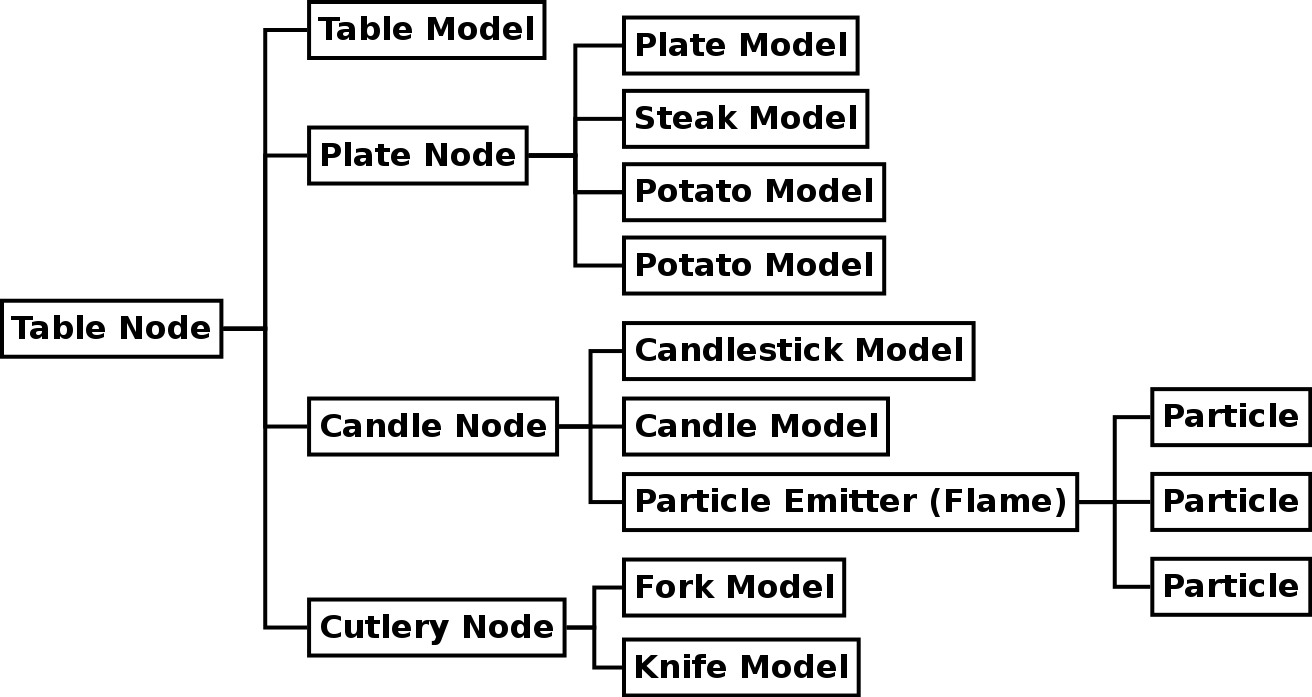
\includegraphics[width=14cm]{images/example-scenegraph.png}
		\caption{An example scene graph depicting a dinner table}
		\label{fig:ExampleSceneGraph}
	\end{figure}

	Apart from these usability features, scene graphs are further useful for the calculation of bounding volumes, which in turn are used for clipping. Assarson et. al summarize several such techniques and shows a speed improvement of up to 11-fold using these methods\cite{Assarsson:2000:OVF:360529.360537}.

\section{Quaternions}

	Positioning an object within a scene graph requires the expression of its orientation relative to its parent node. There are several methods for expressing the attitude of an object within 3-dimensional space, which are summarized in \cite{Diebel06}. The \termdef{quaternion} has become the de-facto standard for this purpose in graphics engines\cite{Mukundan02}, as it is neither as memory-intensive as a transformation matrix, nor prone to the so-called gimbal lock as Euler angles are.

	Quaternions are hyper-complex numbers of rank 4, constituting a four dimensional vector space over the field of real numbers\cite{birkhoff1960survey}. A Quaternion is expressed as a four tuple
	\[q = (w, x, y, z) = w + ix + jy + kz\]
	which consists of a vector part $x, y, z$, the scalar part $w$ and where the units $i$, $j$, $k$ satisfy:
	\begin{gather}
		i^{2} = j^{2} = k^{2} = ijk = -1 \\
		ij = -ji = k \\
		jk = -kj = i \\
		ki = -ik = j
	\end{gather}

	A quaternion expresses an attitude within 3d-space -- more precisely the rotation towards an attitude. The multiplication of quaternions ($A \cdot B$) correspond to sequential application of their rotations and yields a new quaternion ($C$) which expresses the first rotation followed by the second rotation. As the first rotation will rotate the axes of the second rotation, changing the order of the multiplicants results in a different compound rotation, rendering the quaternion multiplication non-commutative. This property of rotations is visualized in Figure \ref{fig:Rotations}.

	\begin{figure}[htbp]
		\centering
		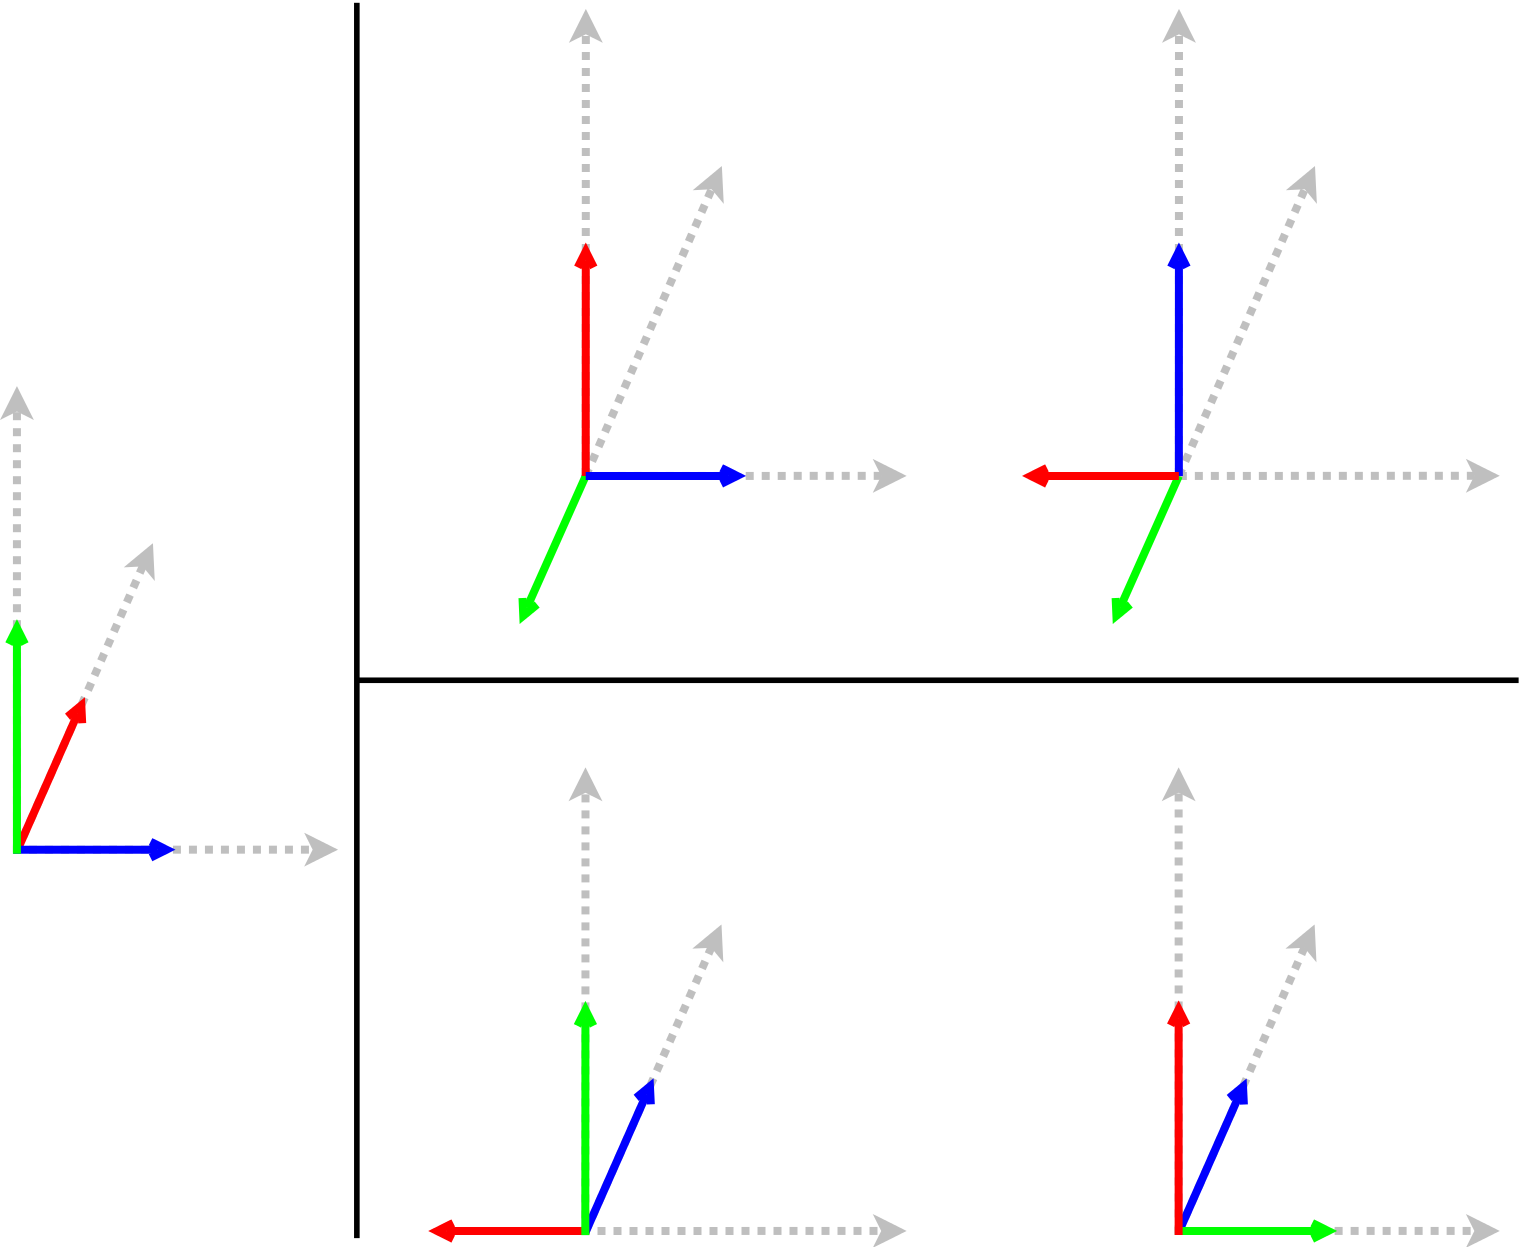
\includegraphics[width=14cm]{images/rotation.png}
		\caption{Changing the order of rotations yields different results: The rotations above (90\degree around blue, 90\degree around green) are applied to the original orientation in reverse order in the lower half, resulting in different final attitudes.}
		\label{fig:Rotations}
	\end{figure}

\section{Render Loop}

	\clubpenalty=10000
	\widowpenalty=10000
	Once the initial setup of a scene is completed, it needs to be drawn onto the screen each time an object in the scene is modified. Instead of rendering the output each time the scene is updated, most graphics engines choose to redraw it in an infinite loop, assuming that the output will change frequently enough that a constant redraw is necessary. This behavior is in contrast to that of window managers for example, which usually redraw the screen only when necessary.
	\clubpenalty=150
	\widowpenalty=150

	There are several aspects to the design of this infinite loop. Valente et al.\ \cite{Valente_Conci_Feijo_2005} list and categorize several such models. The most simple implementation, the ``simple coupled model'', is visualized in Figure \ref{fig:RenderLoopSimple}. The objects are updated with fixed values in this model -- the camera rotates 1\degree each frame, for example.

	\begin{figure}[htbp]
		\centering
		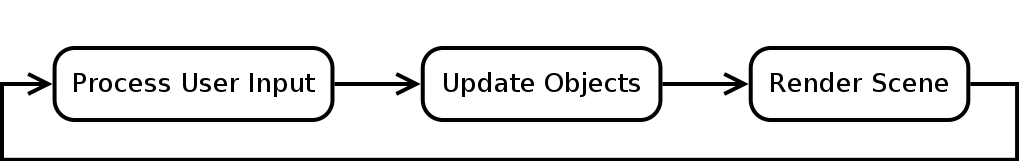
\includegraphics[width=9.25cm]{images/renderloop-simple.png}
		\caption{The most simple render loop}
		\label{fig:RenderLoopSimple}
	\end{figure}

	The disadvantage of this simple design is its dynamic frame rate -- some operations will take longer than others, resulting in greatly varying intervals between single frames, which will result in different results on different hardware. Synchronizing the output of the renderer to a fixed interval is achieved by a simple blocking operation at the end of each cycle as seen in Figure \ref{fig:RenderLoopSimpleSync}. This will guarantee an output at a fixed rate, like 30 frames/second, and allows the developer to use constant values during updates as with the previous model.

	\begin{figure}[htbp]
		\centering
		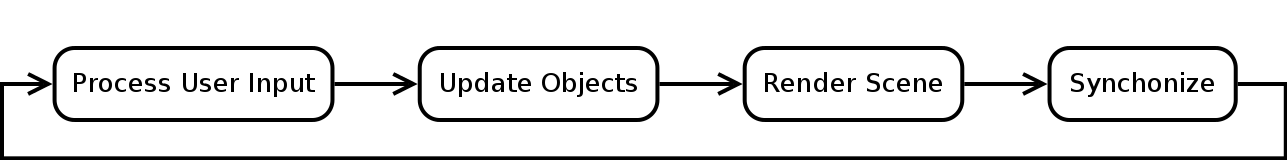
\includegraphics[width=12cm]{images/renderloop-simplesync.png}
		\caption{A simple render loop with synchronization.}
		\label{fig:RenderLoopSimpleSync}
	\end{figure}

	This approach is still insufficient, as the application starts to stutter whenever a cycle needs more time to finish than the predefined time slot. The solution is to perform all modifications to the objects in the scene using the time elapsed since the last cycle. This is the ``Single-thread Uncoupled'' model shown in Figure \ref{fig:RenderLoopDynamic}. It is further possible to add a synchronization to the end of the loop, limiting the required operations to fixed  multiples of the constants required during the loop. If a cycle needs two time slots in the example above (i.e. more than \sfrac{1}{30}, but less than \sfrac{2}{30} seconds), the next cycle will rotate the camera by 2\degree instead of 1\degreenospace.

	\begin{figure}[htbp]
		\centering
		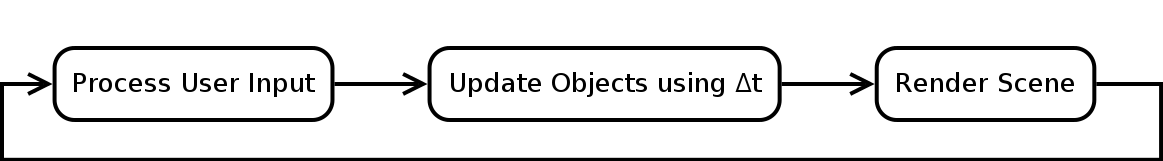
\includegraphics[width=11cm]{images/renderloop-dynamic.png}
		\caption{Single-thread Uncoupled model.}
		\label{fig:RenderLoopDynamic}
	\end{figure}

	Other models operate on multiple threads. Most importantly the rendering is performed in a separate thread, which blocks until the world updates in other threads are in a consistent state. These approaches make use of the multiple CPU cores present in today's hardware. Another big advantage of such models is that the rendering itself is performed on the GPU, while the other operations are usually bound to the CPU. All previously presented models stress either of these resources, while the other stays idle.
	
	It is possible to tackle this issue without the need for threading when using double buffering -- a common feature of modern 3d graphics cards. Most calls to OpenGL will return immediately while processing the issued command on the GPU. The call to the OpenGL function \inlinecode{SwapBuffers()} -- which flushes the rendered image onto the screen -- will block until all pending operations are finished. This makes it possible to perform other operations during this time frame. This approach is outlined in Figure \ref{fig:RenderLoopOpenGL}.

	\begin{figure}[htbp]
		\centering
		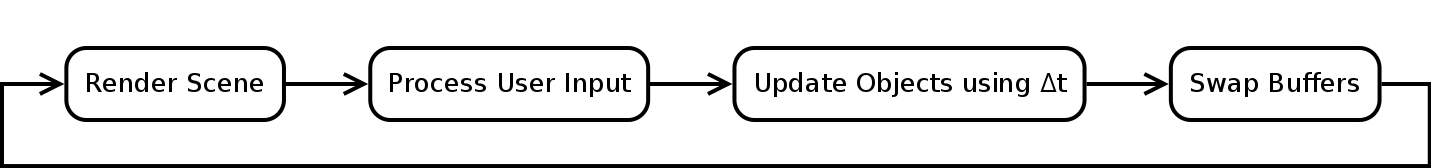
\includegraphics[width=13.5cm]{images/renderloop-opengl.png}
		\caption{A render loop in OpenGL performing operations in parallel on the CPU and the GPU.}
		\label{fig:RenderLoopOpenGL}
	\end{figure}

\section{Models}

	A \termdef{model} is a 3D object that can be positioned in space. Usually models have a predefined shape, a \termdef{mesh}, consisting of a collection of triangle definitions. The mesh alone is not enough to render any realistic scene, additional \termdef{material} definitions are attached to triangle groups which define how the triangles are to be drawn by the renderer. These materials are implemented by dedicated code fragments that run on the GPU. These self-contained applications -- so-called \termdef{shaders} -- are categorized by the objects they operate on\cite{bauchinger-2007-mre}.

	\begin{smalllist}
		\item \termdef{Vertex Shader}s operate on single vertices -- the points in the 3D-space of the mesh forming the triangles -- of the mesh. This shader type receives a single point as input and must operate on that vertex alone without any knowledge of its surroundings.
		\item \termdef{Geometry Shader}s receive multiple vertices that were processed by the vertex shaders. They have the ability to add new vertices or remove/modify existing vertices.
		\item \termdef{Pixel Shader}s (also called \termdef{Fragment Shader}s) operate on the pixels of the final image, just before it is drawn onto the screen. Figure \ref{fig:Shaders} displays a few examples of pixel shaders.
	\end{smalllist}

	\begin{figure}[htbp]
		\centering
		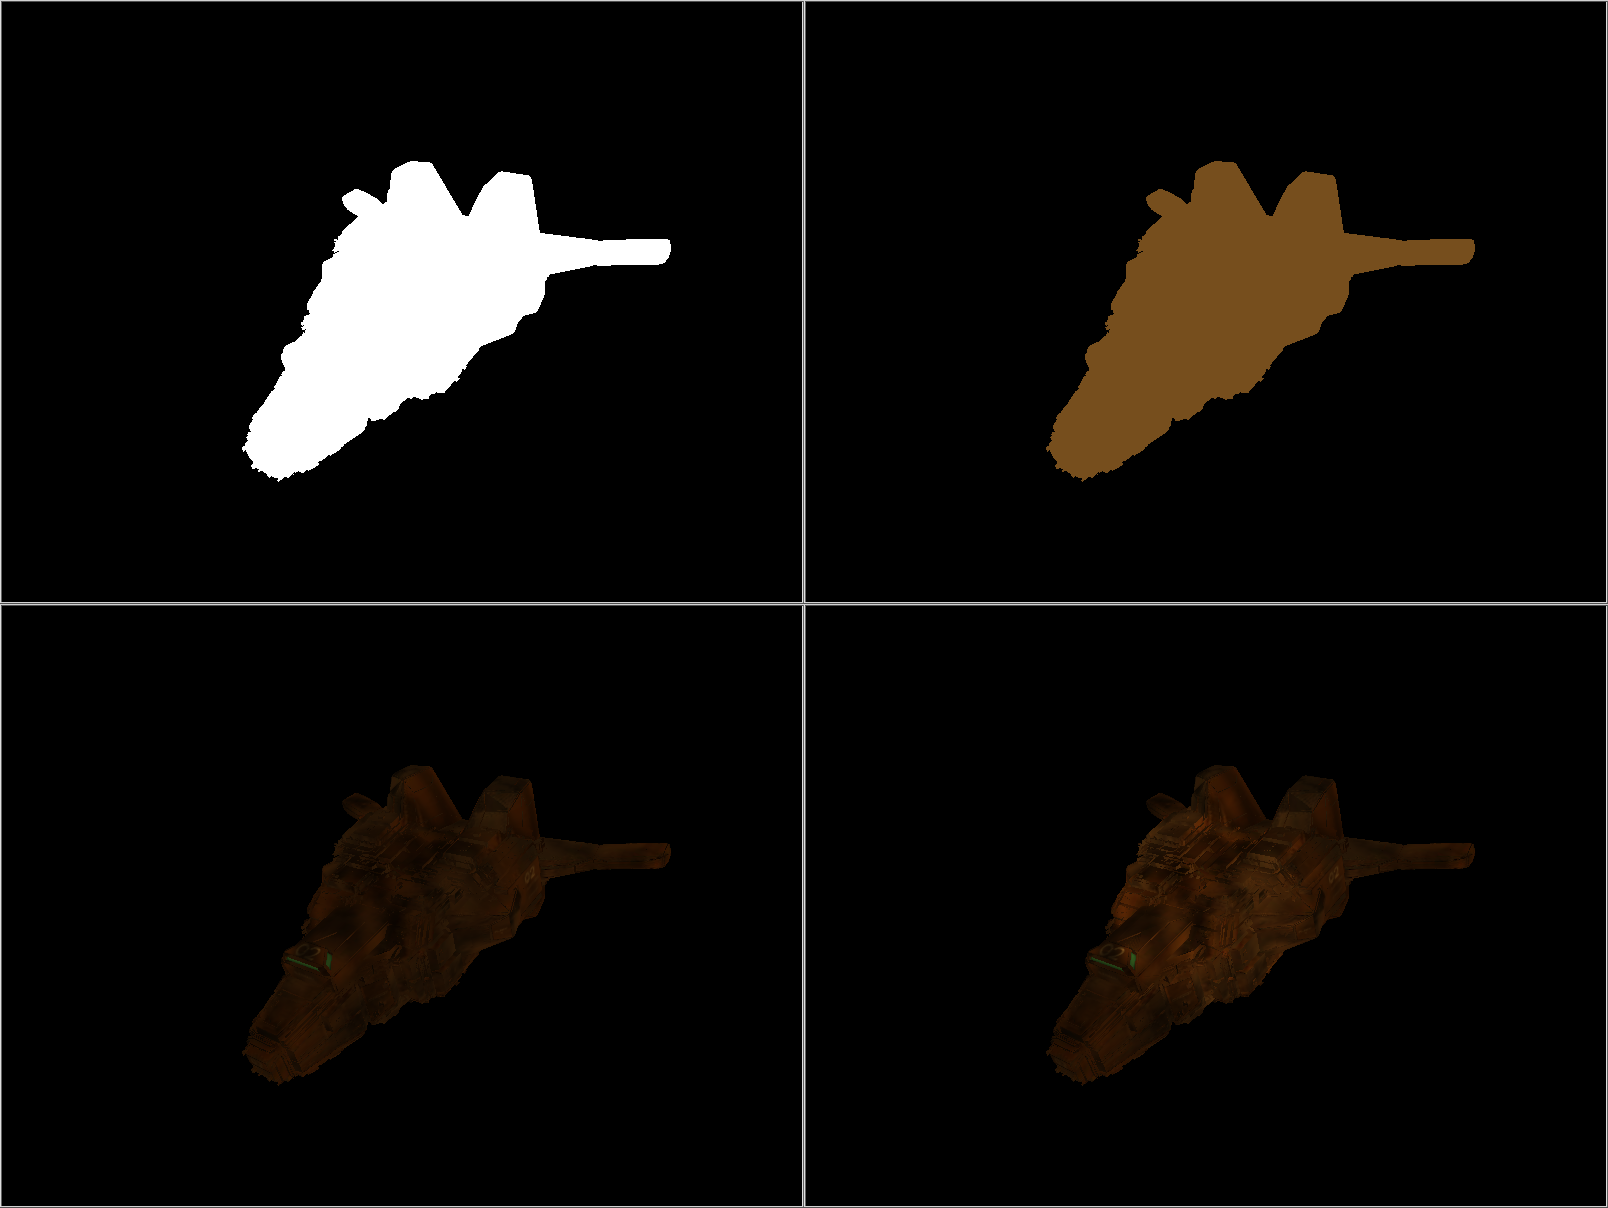
\includegraphics[width=13.5cm]{images/shaders/shaders.png}
		\caption{Examples of pixel shaders: the same model a.) without any shaders, b.) with a uniform color, c.) with a texture and d.) a shader rendering a spotlight onto it.}
		\label{fig:Shaders}
	\end{figure}

	As all of these shaders operate on tiny fragments of the complete scene, the application of the shaders can be run in parallel. Modern graphics cards can run hundreds of operations in parallel for this purpose\cite{Nvi09}.

\section{Lighting}

	Although lights are usually defined as self-contained entities in a scene, they are never drawn directly. Instead, they define how other objects in the scene are rendered. Heidrich et. al. summarize various lighting models in virtual environments in \cite{Heidrich:1999:RHS:311535.311554}. A light source usually consists of two components: diffuse and specular.

	\begin{smalllist}
		\item The diffuse component of a light ray is scattered at many angles upon hitting a surface and can thus be seen from various angles, whereas
		\item the specular component is reflected at the same angle at which it hits a surface.
	\end{smalllist}

	As light sources are only observable by the illumination of the objects in the scene, these two components are defined on the material of all surfaces, too. Whenever a diffuse (or specular) light would illuminate a surface, the material of the surface defines the effect of the illumination. A mirror will almost ignore the diffuse component of the light, but reflect the specular component with the same intensity as the incoming light beam. Most natural fabrics will do the exact opposite.

	Another property of lights is the direction the light beams are emitted towards. The common categories defined by this behavior are:

	\begin{smalllist}
		\item \termdef{point light}s -- unidirectional light sources,
		\item \termdef{spot light}s -- emitting light in a cone,
		\item \termdef{directional light}s -- coming from an infinitely distant point, giving off parallel rays -- and
		\item a single \termdef{ambient light} -- uniformly illuminating everything equally from all directions.
	\end{smalllist}

	The last parameter for light sources is their attenuation behavior -- how the light emitted from a light source is reduced depending on the distance to the surface it illuminates. This is actually rather a property of the environment in which the light source operates, as light does not fade as long as it travels unhindered in vacuum. A dusty room, on the other hand, would cause light sources to be less effective with increasing distance. The attenuation is considered a property of the light source nonetheless for technical reasons: The modification of illumination based on the properties of the sub-spaces between the surface and light source would be quite complex and computationally extremely expensive.

\section{Cameras}

	A camera is a viewpoint from which the scene is rendered. The visible space to a camera is the so-called \termdef{view frustum}\cite{Lengyel:2003:MGP:996316}, and is constrained by the near and far clip distances as seen in Figure \ref{fig:CameraFrustum}. Solely objects within -- or reaching into -- this area are rendered when viewing the scene from this camera.

	\begin{figure}[htbp]
		\centering
		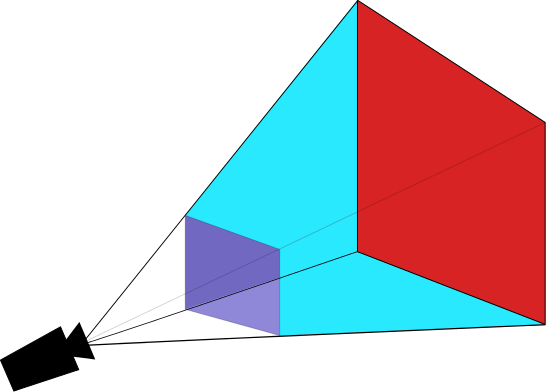
\includegraphics[width=9cm]{images/frustum.png}
		\caption{The view frustum of a camera, contained by the \emph{near clip distance} in purple and the \emph{far clip distance} in red.}
		\label{fig:CameraFrustum}
	\end{figure}

	The other two parameters for the definition of a camera are its field of view -- the horizontal angle of the frustum -- and the aspect ratio defining the vertical angle. It is possible to establish further properties that simulate the effects of different camera lenses\cite{Kolb:1995:RCM:218380.218463}, but we will limit our model to the simplified definition above.


	\chapter{Scope}
	\section{Reference Engines}

	Throughout the thesis, we will have other graphics engines as reference implementations and API examples. We have chosen three different engines with varying aims as such reference engines:

	\begin{smalllist}
		\item OpenSceneGraph: This engine features a very powerful but complex scene graph implementation. The complete design philosophy is focused on the scene graph, the data structure managing the objects within the scene. This data structure is very important in modern graphics engines and will be explained a bit more in the next chapter. The API of the engine itself is targeted at developers with experience in the graphics domain and it is quite complex, requiring good knowledge of the math behind the scenes. An introduction to the engine can be found in \cite{OpenSceneGraph22}.
		\item Panda3d: Initially produced by Disney’s VR Studio, this engine has become an open source project that is still used in commercial projects of Disney\footnote{\emph{Toontown} (http://toontown.go.com/) and \emph{Pirates of the Caribbean online} (http://piratesonline.go.com/welcome) being two examples}. The engine itself is developed using C++, but the engine comes with a python interface allowing rapid prototyping without the need for recompilation \cite{Goslin:2004:PGE:1032275.1032359}. We have found that it has indeed a very clean and simple API that allows the creation of simple scenes with few commands.
		\item Ogre3d: A quite popular open source graphics engine that was used in several commercial games. According to its web page, it was ``designed to make it easier and more intuitive for developers to produce applications utilizing hardware-accelerated 3D graphics''\footnote{http://www.ogre3d.org/about}. Although the API is quite verbose, it has a very clean architecture and good documentation.
	\end{smalllist}


	\section{Features}

	In order to keep the focus on the architectural design within the engine, we will implement a very limited feature set. We will use the topics covered by some introductory books on graphics engine usage to determine these features: \cite{stein2011irrlicht}, \cite{kerger2010ogre}, \cite{mathews2011panda3d}, \cite{Eberly:2006:GED:1214590} and \cite{Martz_2007}. All five books are targeted at developers without prior knowledge of graphics engines and four of them introduce the reader to the API of one specific graphics engine. Although all of them cover many more topics, the common areas can be summarized as:

	\begin{smalllist}
		\item scene graph manipulation,
		\item camera manipulation,
		\item lighting,
		\item loading and manipulating objects (including meshes, materials, textures),
		\item operations on a 2-dimensional space,
		\item processing user input and
		\item usage of the engine within a render loop.
	\end{smalllist}

	Other areas found in more than one of these books are:

	\begin{smalllist}
		\item picking objects,
		\item particle effects,
		\item loading terrain,
		\item collision detection and
		\item visual post-processing.
	\end{smalllist}

	Having a list of common topics in introductory books, we can now pick a set of features that will be included in PURGE.

	\subsection{Renderer}

		The most important decision to make first is the low-level graphics API to use. We could make use of OpenGL or DirectX, but this approach would not provide a good base for benchmark comparisons, as the rendering process is extremely complex and the required optimizations would cover much more ground than the API itself.

		Instead, we will be using the API of other graphic engines. PURGE will solely handle the high-level scene layout and delegate all rendering operations to another, external renderer. This approach will allow us not only to concentrate on the API, but will further provide the ability to compare performance metrics of the resulting library to those of the unmodified renderer.

		Details on the design of this architecture are provided in Section \ref{chapter:design:renderer}, whereas the implementation details can be found in Section \ref{chapter:implementation:renderer}.

	\subsection{Scene Management}

		First, it is important to note that all covered engines make use of scene graphs as a means of managing objects in 3-dimensional space. We will need to define a set of operations we want to support on the nodes of this scene graph. The common properties of the above graphics engines are

		\begin{smalllist}
			\item location,
			\item rotation and
			\item scale.
		\end{smalllist}
		
		Changing the \termdef{Location} of an object ``moves'' the object by a given amount. The \termdef{Rotation} does not change its location per se, but moves all points of an object around an axis in a circular manner.

		The \termdef{Scale} of an object is defined as adjusting the distance of each point of an object to a given point of reference by a scalar. The scale is defined separately for each coordinate axis and can be negative. The complete scale can thus be defined by a tuple of three scalars, one for the scale of each coordinate axis. This implicitly defines a mirroring feature: Scaling by \vect{1}{1}{-1} results in the object being everted along the Z-axis.

	\subsection{Lights}

		Lighting is the feature that affects the realism of a scene the most. As implementing a decent lighting model would go way beyond the scope of this thesis, we will use an extremely simplified model. The light sources in the final library will be defined by

		\begin{smalllist}
			\item a specular color,
			\item a diffuse color and
			\item a linear attenuation value.
		\end{smalllist}

		These parameters define the ``behavior'' of light rays which are emitted from a light source. Another component of light sources is the direction these rays are emitted towards. The types of light present in most engines are

		\begin{smalllist}
			\item point lights,
			\item spot lights,
			\item directional light and
			\item a single ambient light.
		\end{smalllist}

		The first two light sources -- point and spot lights -- can be integrated into the scene as tangible objects. They can be positioned, rotated and scaled as defined by the scene node operations above. Although rotating a point light has no visual effect on the output, it is possible that the rotation has an effect on other objects that are attached to this light source, as we will discuss in Section \ref{chapter:design:scenegraph}.

		The other two light sources -- directional and ambient lights -- are not integrated into the scene graph, but rather defined outside of it as global illumination parameters. As these light sources do not have a single point as origin, they do not have any attenuation either. The sun is a good example of a directional light source that emits light in a single perceived direction, and has no significant attenuation. The ambient light can be thought of as the illumination resulting from diffuse reflections within the scene.

		The design of the light classes can be found in Section \ref{chapter:design:scenegraph}.

	\subsection{Models}

		The final area to be covered is the loading of models into the scene. Although every graphics engine supports various formats, each of them supports reading a geometric model from external resources - most commonly files. Our reference engines are not limited to models when loading entities from files. They have own scripting languages or exporters that can be used to define other object types that can be loaded into the scene. These entities are not necessarily handled by the engine, they might as well be processed by plug-ins. Some examples include
		
		\begin{smalllist}
			\item light sources,
			\item billboard effects,
			\item particle effects,
			\item dynamically generated models (trees, for example),
			\item terrain and
			\item sky boxes.
		\end{smalllist}

		To cope with this variety of entities, the object model of PURGE will not distinguish effects from predefined or dynamically generated models. All loadable objects are treated equally. This decision has one important implication: The resulting library will not be able to manipulate these objects. It is capable of triggering the loading of an object by its name, but incapable of altering an object that was loaded this way. This fact further implies that light sources integrated as ``models'' are indistinguishable from other objects and cannot be modified at a later time.

\section{Excluded Features}

	To further define the boundaries of the engine, we will establish another list of explicitly excluded features; especially since several features not covered in this thesis might be perceived as inherent features of a graphics engine.

	\begin{smalllist}
		\item Rendering to anything except the screen: Rendering to the screen is assumed to be the primary concern of a developer making use of such a simplistic API,
		\item 2d objects: Neither the rendering of menus, nor any other two-dimensional overlays are covered in this thesis. The focus will be solely on the management of the three-dimensional scene.
		%\item Interaction: The resulting engine is not able to process any user input.
			%Management of user input is another broad topic that is 
			%There is just one exception to this rule: it can react to the closing of a render window.
	\end{smalllist}


	\section{Use Cases}

	As the target audience consists of software developers with little or no prior experience with graphics engines, the library will provide the most convenient API for the simplest tasks. We considered the following list to be the most rudimentary tasks when confronted with a graphics engine API for the first time:

	\begin{smalllist}
		\item Creating an empty scene and looking into that scene through a camera: This step involves the creation of all necessary objects to enter the rendering loop. As this step is part of every application, the reduction of this boilerplate code could be considered to be the most important use case.
		\item Positioning an object in the scene: Loading an object into the scene and altering its coordinates, orientation and/or scale to be visible through the default camera.
		\item Updating an object: Moving, rotating or otherwise modifying a previously loaded object discretely in a pre-defined time period.
		\item Controlling the camera: Updating properties of the camera, enabling the implementation of a dynamic scene.
	\end{smalllist}

	This list of use cases will be used during the evaluation of the final architecture in Section \ref{chapter:evaluation:tests}.


	\chapter{Design}
	Since the aim of this thesis is to provide an API usable without domain-specific knowledge of computer graphics, the API will try to hide as many domain-specific aspects of graphics engine usage as possible. It will need to predict some intentions of its users. For example, the library will automatically create a render window if none was created by the user before the render loop was entered. More such details are summarized in Section \ref{chapter:implementation:loop}.
%It will allow attaching a camera to a render window, implicitly creating a viewport with maximum width and height during this operation.

It will further try not to hide away such implementation details completely, giving more experienced developers the level of control available in other graphics engines. This approach effectively creates an API that is usable on two levels:

\begin{smalllist}
	\item as a complex, feature-rich graphics engine, and
	\item as a simplified engine with many default parameters and operations.
\end{smalllist}

The driving force behind any decisions during the design process was the principle of least astonishment\cite{Saltzer:2009:PCS:1594884}. The adopting developers are assumed to be developers that have very little or no prior knowledge of implementing graphics applications, which implies that some behaviors of the resulting engine might still be unexpected to those knowledgeable in this domain. An experienced developer might want to enter the render loop without any active render windows, for example.

To support these operations, all automatic behavior will be modeled to be suppressible. It is still possible to start the main rendering loop without any target to render to if this is the actual intent. But, where other engines would insist on a choice -- and would probably abort execution due to a lack thereof -- PURGE instead tries to make that choice for the developer. This naturally means that the choice might not be the right one for users familiar with this domain.


	\section{External Renderer}
\label{chapter:design:renderer}

	Luckily, the usage of an external renderer already provides access to an advanced API. Users knowledgeable about the external graphics engine being used can fine-tune operations within that engine. Any object controlling the rendering process is created within the PURGE namespace, and adopted by the external rendering facility, the \classname{Renderer}. That facility is responsible for taking that object into account during the rendering process.

	\begin{figure}[htbp]
		\centering
		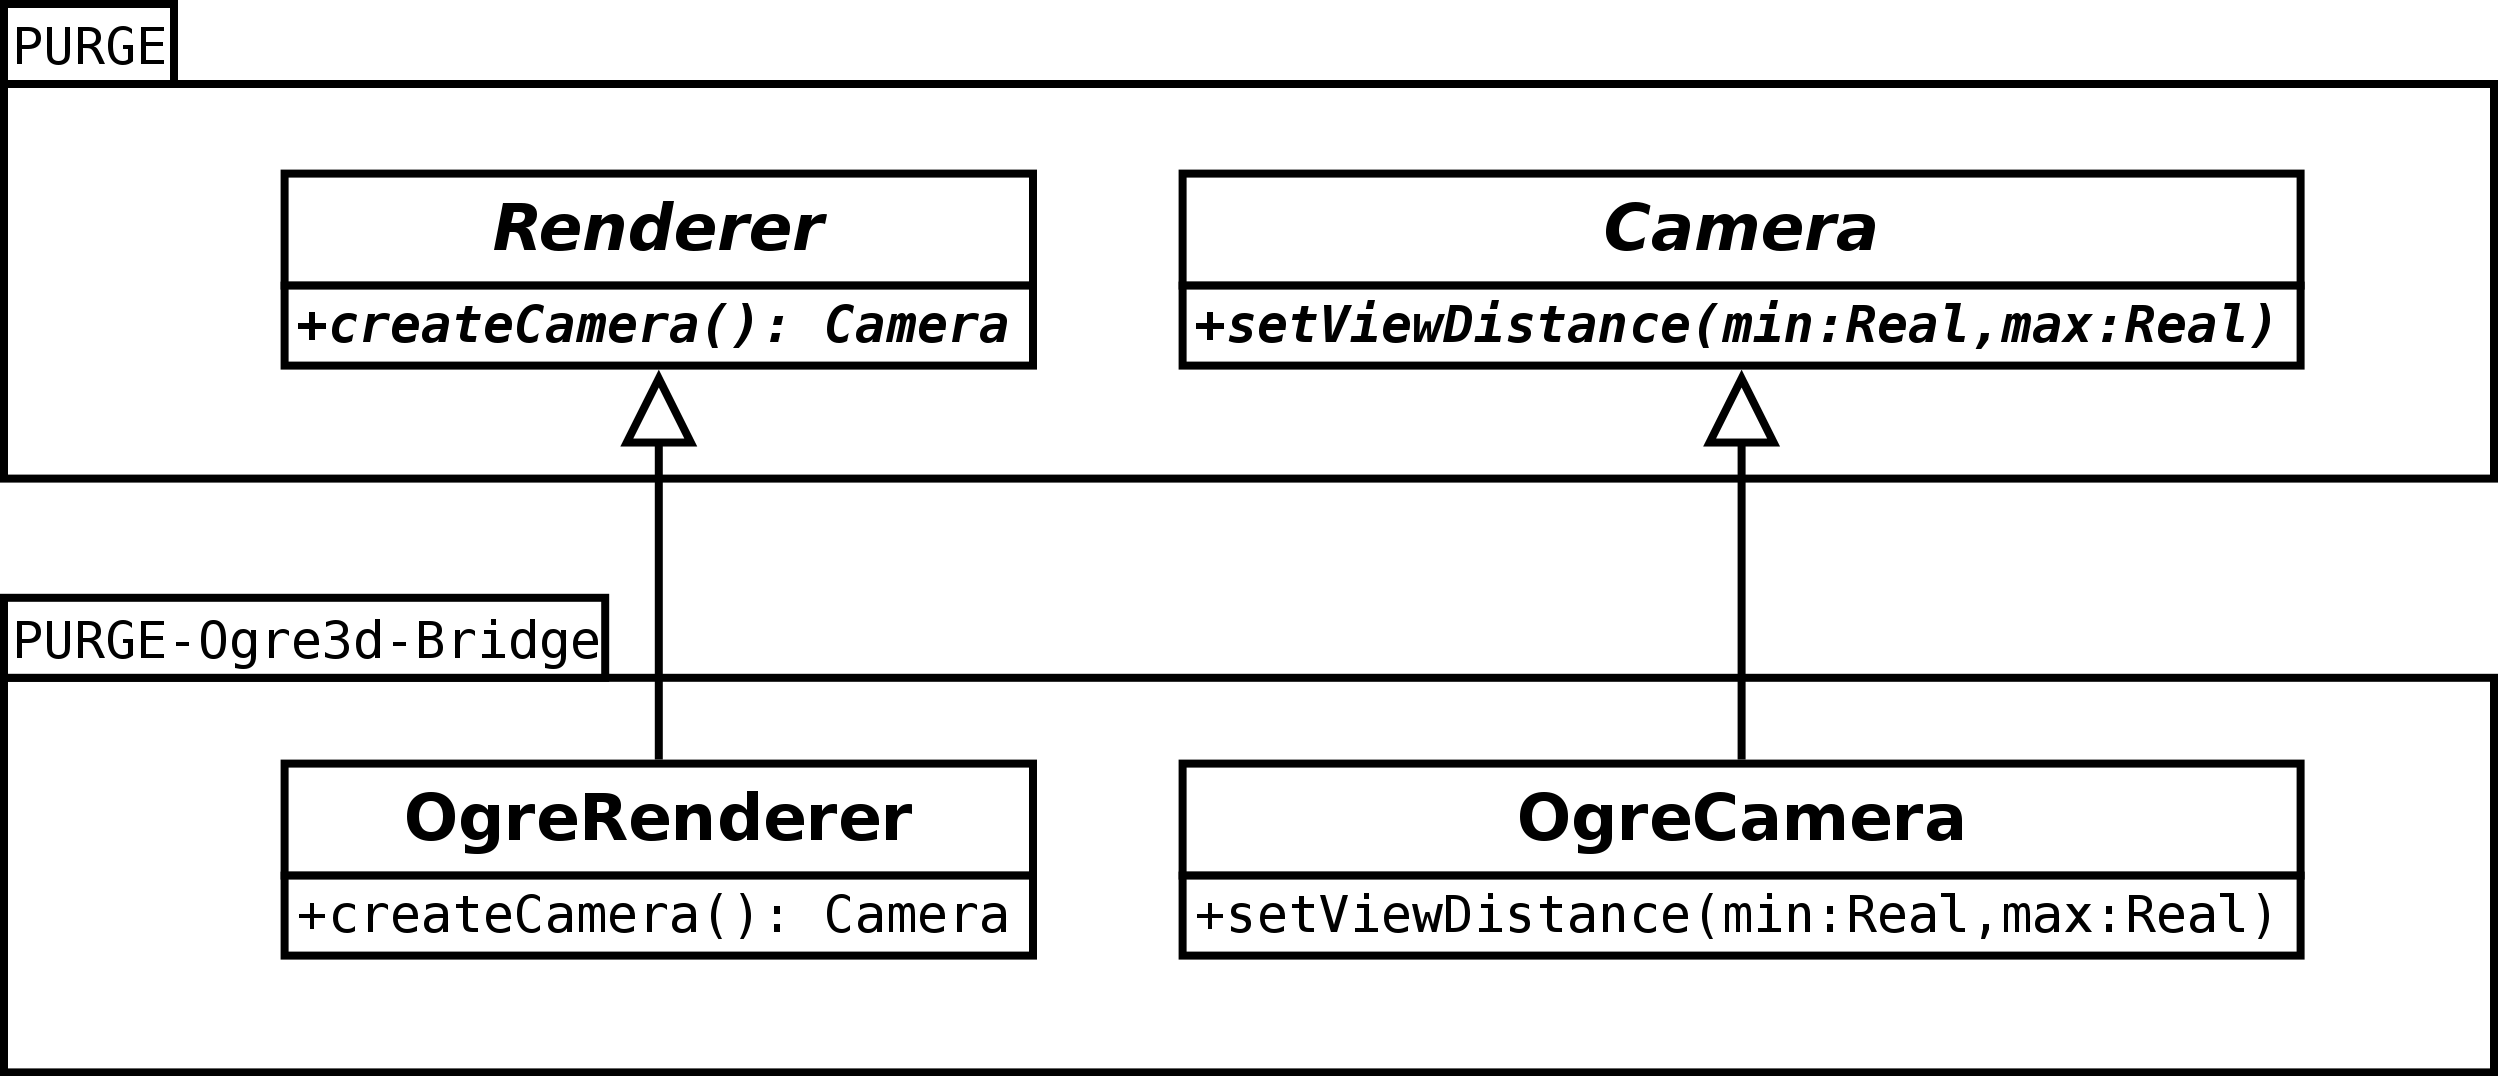
\includegraphics[width=14cm]{images/RendererArchitecture1.png}
		\caption{Initial design approach to the external renderer}
		\label{fig:RendererArchitecture1}
	\end{figure}

	The first approach to the integration of the external render was to design the \classname{Renderer} as an abstract class that is responsible for providing all other objects supported by PURGE, as seen in Figure \ref{fig:RendererArchitecture1}. The drawback of this architecture became clear quite early during the implementation process: The design of PURGE was adopting too many characteristics of the underlying renderer. The library was becoming a layer on top of Ogre3d instead of an independent graphics library.

	To counter this trend during the design process, the architecture was slightly altered to decouple PURGE objects from their implementations in the renderer. The aim was to render the \classname{Renderer} completely interchangeable, even at run-time, an approach to the engine design we have found in \cite{Plummer2004}\footnote{Plummer basically contemplates on a game architecture proposal in \cite{Rollings:2003:GAD:1209229} and attempts to create a game engine with completely interchangeable components for specialized tasks.}. This has lead to the second design outlined in Figure \ref{fig:RendererArchitecture2}, where the objects in PURGE can survive an exchange of the active \classname{Renderer}. We switched from direct inheritance to the bridge pattern as described in \cite{GOF}.

	\begin{figure}[htbp]
		\centering
		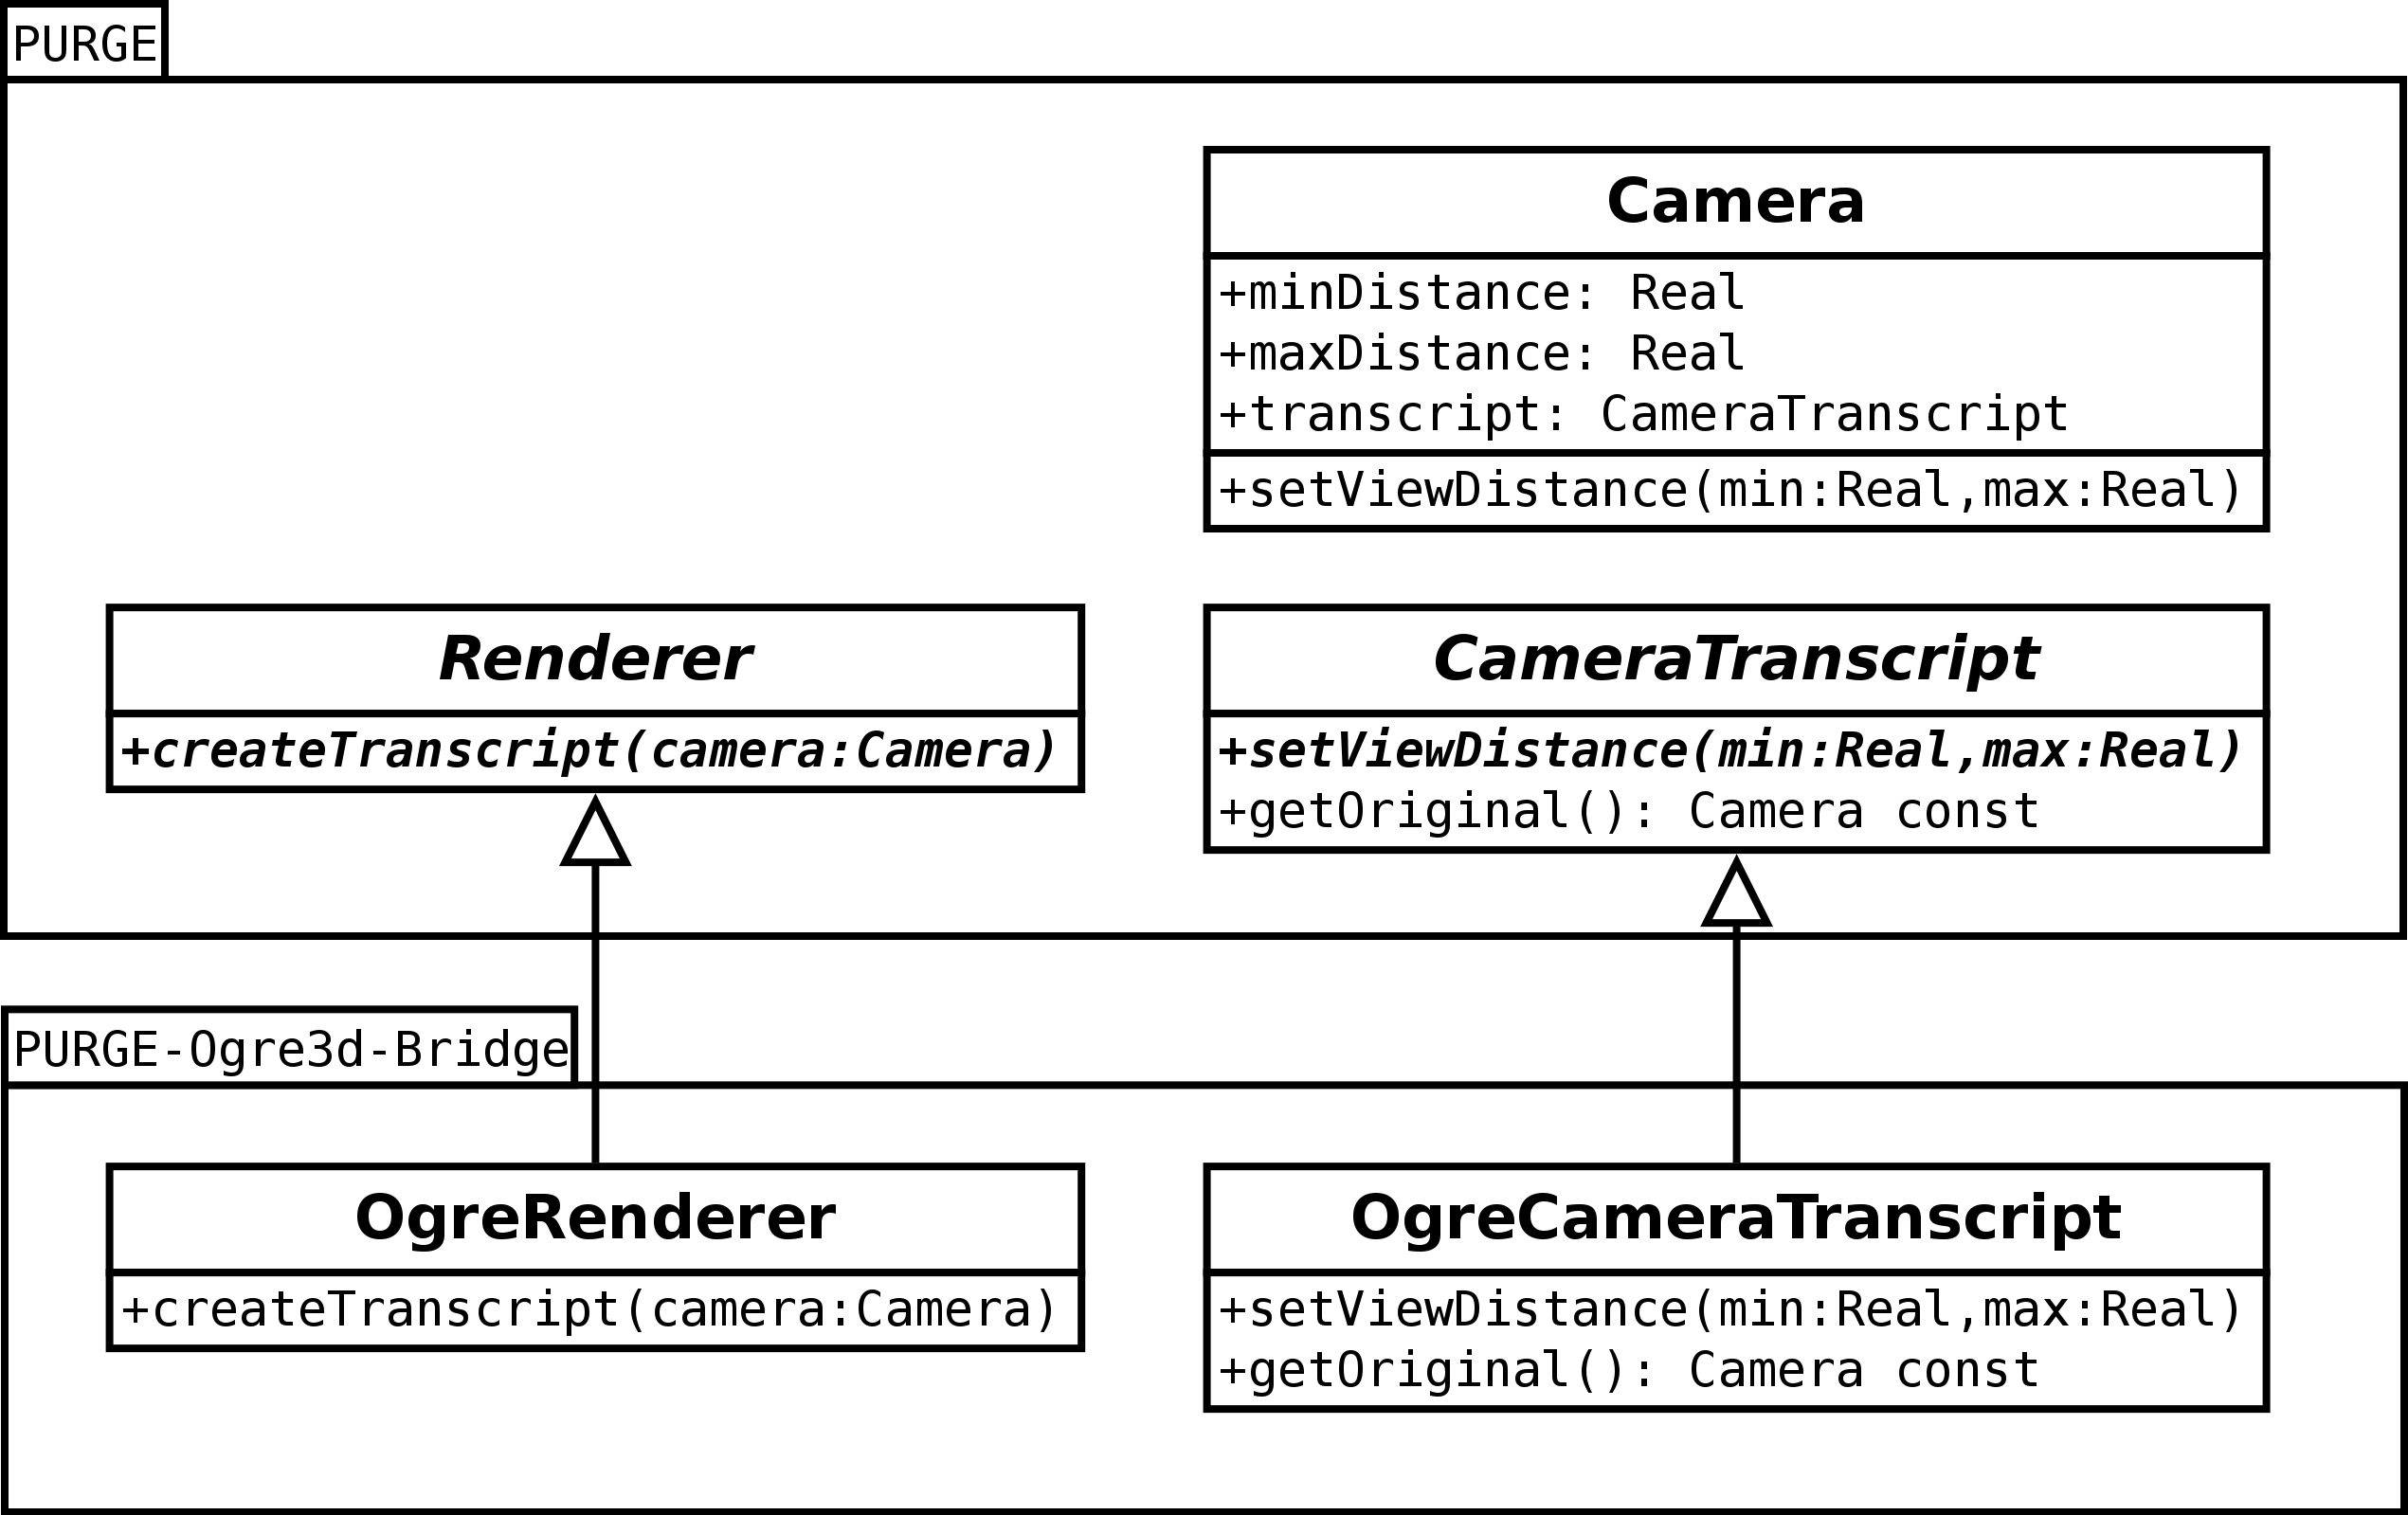
\includegraphics[width=14cm]{images/RendererArchitecture2.png}
		\caption{Second design of the external renderer}
		\label{fig:RendererArchitecture2}
	\end{figure}

	But this change had some drawbacks: Although the PURGE object was now capable of storing its parameters, the API had not changed. The object would now store its state on its own, but immediately update the implementing object. Apart from this lack of solution to the initial problem, another, more grave design flaw was brought to our attention with this switch. Why should the library actually enforce the duplication of the already-present data in the \classname{Renderer}?
			
	What was the \classname{Transcript} good for? It was a required implementation detail in the initial design, but the usage of the bridge pattern had made that class obsolete for PURGE. The \classname{Renderer} was still free to create a mapping of a PURGE-object to its own, graphics-engine specific objects, but PURGE does not need any information from these objects.
	
	So this short-lived solution was discarded and the flow of information was reversed: Instead of pushing any changes from PURGE to the \classname{Renderer}, the \classname{Renderer} is now expected to pull any information it needs from PURGE. The outline of this design can be seen in Figure \ref{fig:RendererArchitecture3}.

	\begin{figure}[htbp]
		\centering
		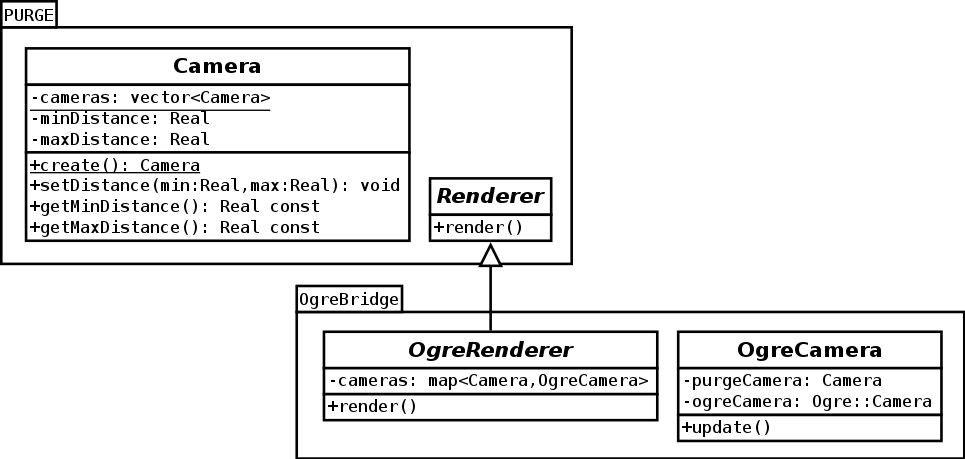
\includegraphics[width=14cm]{images/RendererArchitecture3.png}
		\caption{Third iteration of the renderer architecture}
		\label{fig:RendererArchitecture3}
	\end{figure}

	With this last change, the flow of information is defined as follows:
	
	\begin{numlist}
		\item The application can create, update and delete any number of objects in PURGE. None of the changes have any visible effect at this point.
		\item When all changes for this loop cycle are declared to PURGE, the rendering step initiates.
		\item The \classname{OgreRenderer} is responsible for creating, updating and deleting all required internal objects to render the scene as contained in PURGE.
		\item When the renderer is finished, control is passed back to PURGE, where a new loop cycle begins.
	\end{numlist}

	The implementation of this communication model requires further elaboration on the details of the render loop. We will come back to the implementation specifics in Section \ref{chapter:implementation:renderer}.


	\section{Render Loop}
\label{chapter:design:loop}

	The communication between PURGE and the external \classname{Renderer} is heavily dependent on the render loop -- or main loop -- of our library. The loop basically consists of three different stages that need to be run through repeatedly:

	\begin{numlist}
		\item gathering user input,
		\item updating the scene and
		\item rendering the scene.
	\end{numlist}

	We will be using the ``Single-thread Uncoupled model'' presented by \cite{Valente_Conci_Feijo_2005}, which cycles through these stations periodically in a single thread and updates the objects using the time elapsed since the last cycle. We will see in Section \ref{chapter:implementation:loop}, that the choice of the implementation does not have a strong impact on the API.

	The render loop in a graphics engine must provide an API for the repeated modification of the scene by the application. The sequence described above (gather input, update, render) is present in all reference engines, but each of them approaches this problem quite differently:

	\begin{biglist}
		\item Ogre3d: Provides the FrameListener interface\footnote{http://www.ogre3d.org/docs/api/html/classOgre\_1\_1FrameListener.html} for the registration of recurring tasks during the loop cycle. Developers can implement this interface to react to certain events in the rendering loop, usually the end of the render cycle. The current version provides three such events:

		\begin{smalllist}
			\item \inlinecode{frameStarted()}: Called before the frame is being rendered.
			\item \inlinecode{frameRenderingQueued()}: Called while the GPU is computing the current frame. This event is useful in the case one wants to make use of the CPU at this time, as the CPU would otherwise be idle and the application would block until the GPU is finished.
			\item \inlinecode{frameEnded()}: Called after the rendering is finished.
		\end{smalllist}

		Ogre3d does not have native routines for processing input from external devices (such as keyboards or mice), but an external project is recommended for this purpose throughout the documentation: OIS\footnote{The official web-site of the project is http://www.wreckedgames.com, but more information can be found on its sourceforge project site: http://sourceforge.net/projects/wgois/}. This external library again provides two methods of processing input: buffered and unbuffered. If the library is used in buffered mode, all input can be processed at once during the execution of a frame listener. In unbuffered mode, a listener has to be provided to the library that will be called immediately on the retrieval of new events through system interrupts.

		\item Panda3d: Allows the registration of tasks to be continuously performed at a central facility, the \classname{AsyncTaskManager}. As the name suggests, the library is capable of distributing ongoing tasks across different threads and actually makes use of this mechanism to manage the rendering loop. The rendering step itself is nothing more than a \classname{GenericAsyncTask}. A nice option is the registration of function pointers instead of full-blown classes, which makes playing around with the library a bit more convenient.

		The \classname{AsyncTaskManager} holds multiple instances of \classname{AsyncTaskChain}, which contain objects of type \classname{AsyncTask}. Each \classname{AsyncTaskChain} can run in a separate thread. Furthermore, each \classname{AsyncTask} has a sort number that ensures that tasks can be executed in a predefined order across all \classname{AsyncTaskChain}s. Figure \ref{fig:PandaTasks} visualizes the sequence in a single cycle with two \classname{AsyncTaskChain}s.

		Unfortunately, the name \classname{Chain} is a bit misleading in this context. The name suggests a linear dependence between ``links'', which is not the case: The ``links'' in the chain have additional dependencies to other links in other chains, as seen in Figure \ref{fig:PandaTasks}. A more accurate visual representation of this approach would possibly be ``thread'', reminding of the computational thread it possibly runs in and the thread of a woven fabric, having dependences to other threads.

		\begin{figure}[htbp]
			\centering
			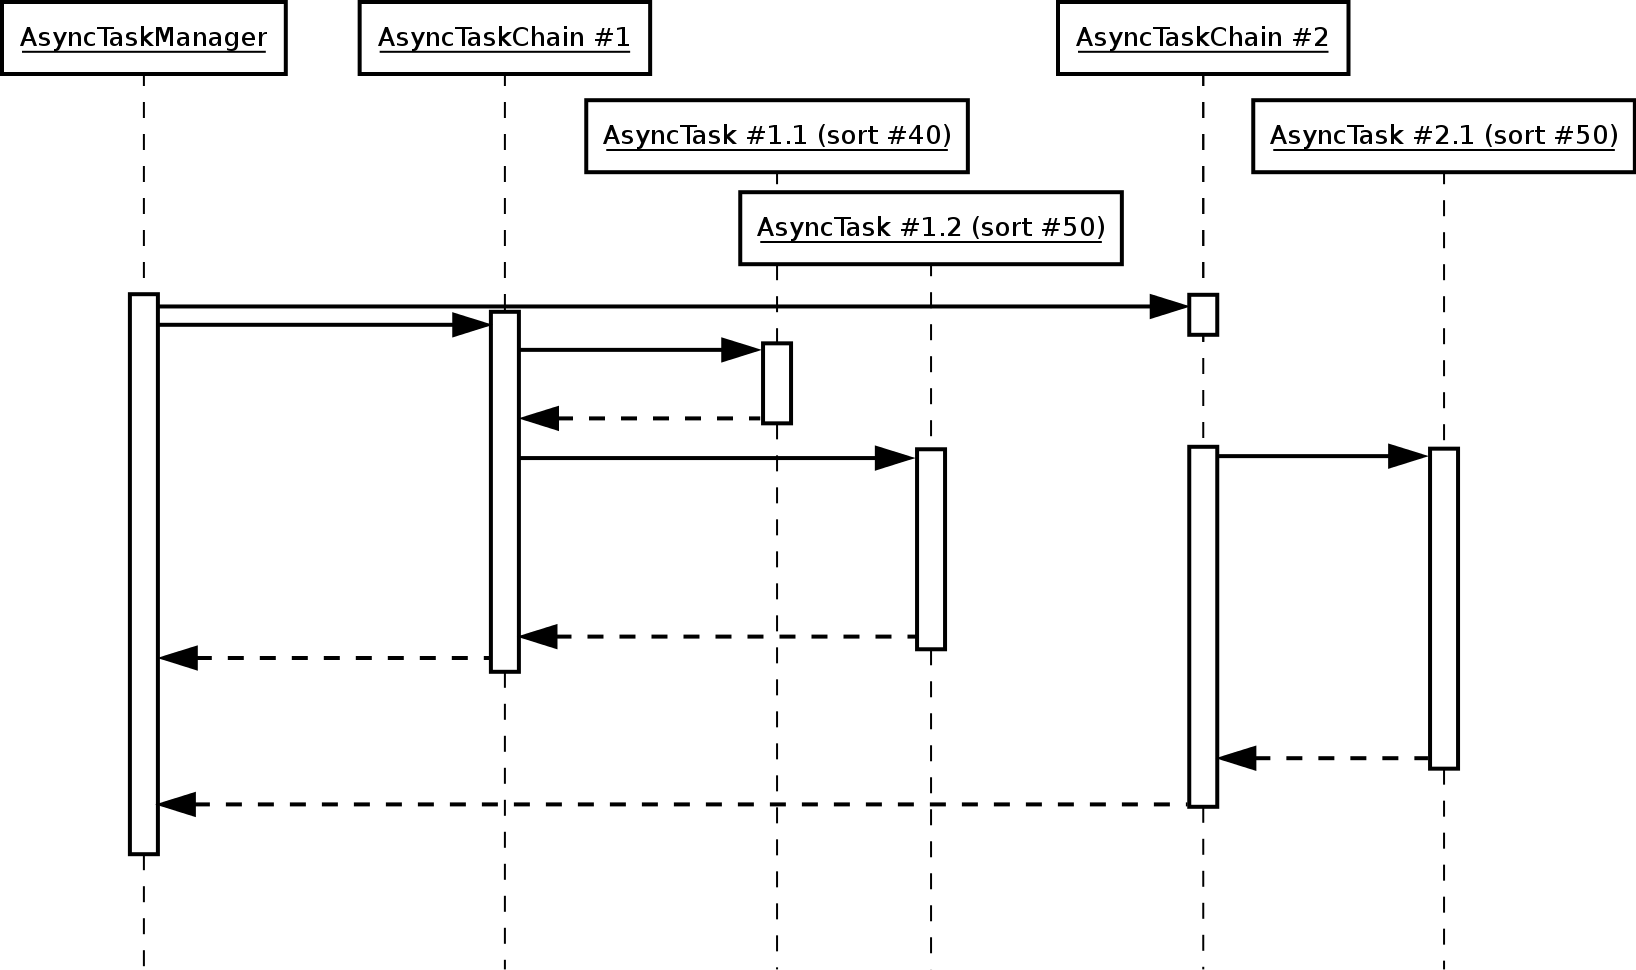
\includegraphics[width=14cm]{images/PandaTasks.png}
			\caption{Simplified sequence diagram of a single rendering cycle in Panda3d. \inlinecode{AsyncTaskChain \#1} and \inlinecode{AsyncTaskChain \#2} start running simultaneously, but the second chain will block until the first task in the first chain was executed, as it has a smaller sort value than the task in the second chain.}
			\label{fig:PandaTasks}
		\end{figure}

		\item OpenSceneGraph: As the project does not provide a render loop \emph{per se}, it is possible to implement ones own loop that takes care of any operations in-between the rendered frames.
			
			But another peculiarity of OpenSceneGraph is the strong focus on the scene graph, even when designing the application flow. We had seen that the scene graph is actually a data structure for organizing objects in space. OpenSceneGraph additionally allows the registration of callbacks to scene nodes. These \classname{NodeCallback}s\footnote{http://www.openscenegraph.org/documentation/NPSTutorials/osgFollowMe.htm} are called during the rendering process as part of the render loop that updates the scene graph.
		
	\end{biglist}

	Among the analyzed libraries, Panda3d provides the most flexible API for managing the scene during the main loop. It allows us to split the loop into multiple threads, making good use of multiple CPUs, but the API emphasizes an early decision which tasks could be performed in separate threads. It requires the definition of \classname{AsyncTaskChain}s for the integration of new tasks into the loop. A dependence between the tasks is then established through the so-called sort numbers.

	An alternative implementation could hide away the details of threading just by introducing Task groups as outlined in Figure \ref{fig:Task}. A Task group adopts the duty of the numeric sort number in Panda3d's loop design. Instead of assigning a value to a task, it is instead added to the same task group as other tasks that can be processed simultaneously.
	
	\begin{figure}[htbp]
		\centering
		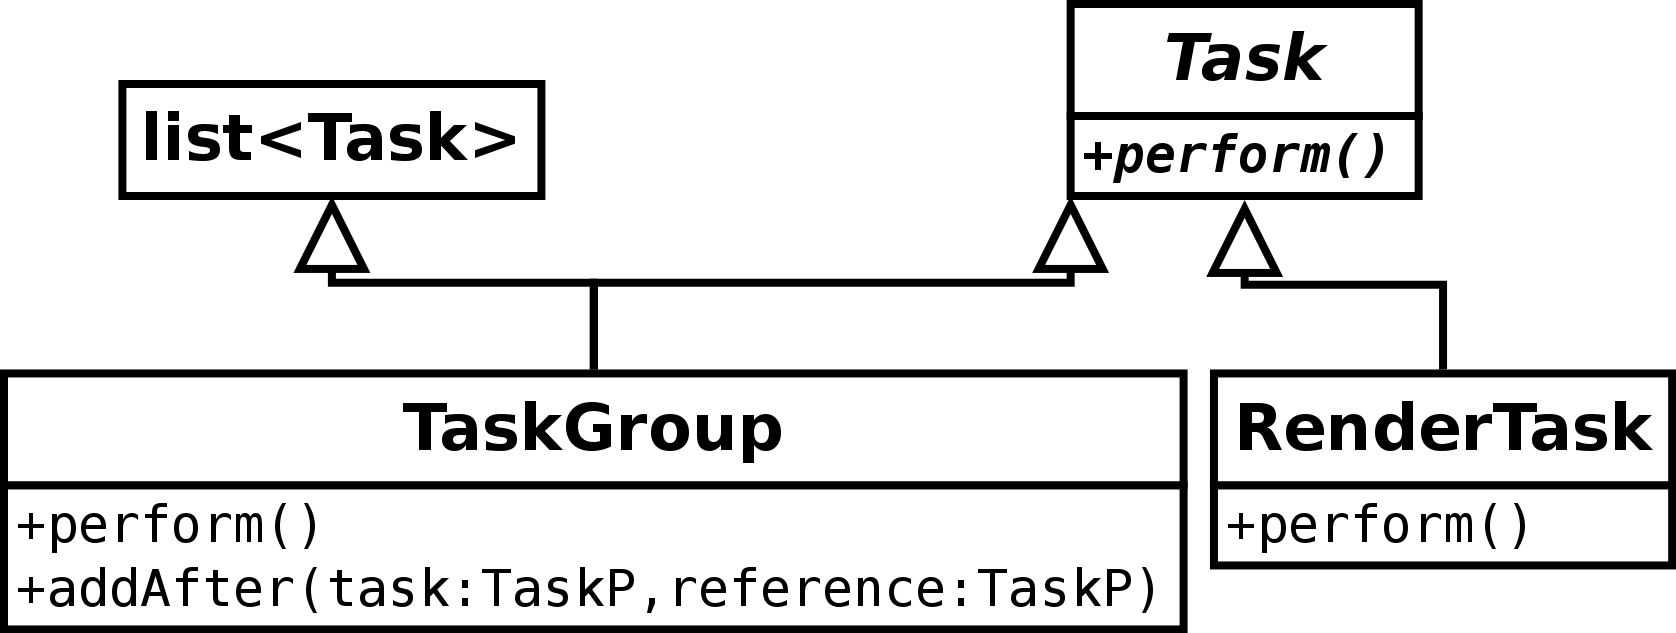
\includegraphics[width=10cm]{images/Task.png}
		\caption{\classname{Task} and \classname{TaskGroup} class hierarchy.}
		\label{fig:Task}
	\end{figure}

	This implementation is in contrast to Panda3d's implementation choice, as it does not group tasks by their ability to run in parallel, but rather creates groups of tasks that need to be performed sequentially -- handling input, computing Physics, computing AI choices, updating positions, and rendering are some examples of such task groups.

	The design described above is equivalent to having a single flat rendering loop that executes tasks sequentially. The \classname{TaskGroup} structure is introduced for convenient re-arranging of the loop elements as a tree structure. With an adequate \classname{TaskGroup} re-implementation it would be further possible to insert parallelism into this design. Although this implementation is not accomplished within this thesis, we will look at it briefly in Section \ref{chapter:implementation:loop}.

	To further simplify the process of adding Tasks to a task group, we will add additional functions to the \classname{TaskGroup} class. These functions will further improve the usability by reducing the number of calls necessary to perform common operations: Adding a task after another reference task, for example.

	While looking into the implementation of the communication between PURGE and the \classname{Renderer} in Section \ref{chapter:implementation:renderer}, we will further discuss the single mandatory task of the library: the \classname{RenderTask}.


	\section{Cameras and Windows}
\label{chapter:design:windows}

	%\cite{Kolb:1995:RCM:218380.218463} provides a very good introduction to the advanced usage of cameras in virtual environments. 

	We will implement a simplified model of cameras, defined by near- and far clip distances, as well as a field of vision. The aspect ratio will always match that of the render window, preventing accidental distortion of the render output.

	A window is a 2d-plane where the view of a camera can be projected to. As the window is partially managed by the system's window manager and modified by the user of an application, this entity should additionally be regarded as a communication device. The user can move, re-size or close the window. We will only model a single such interaction to prove that the architecture could support others as well. Window objects in our library will be able to detect when the user has closed a window.
	
	\begin{figure}[htbp]
		\centering
		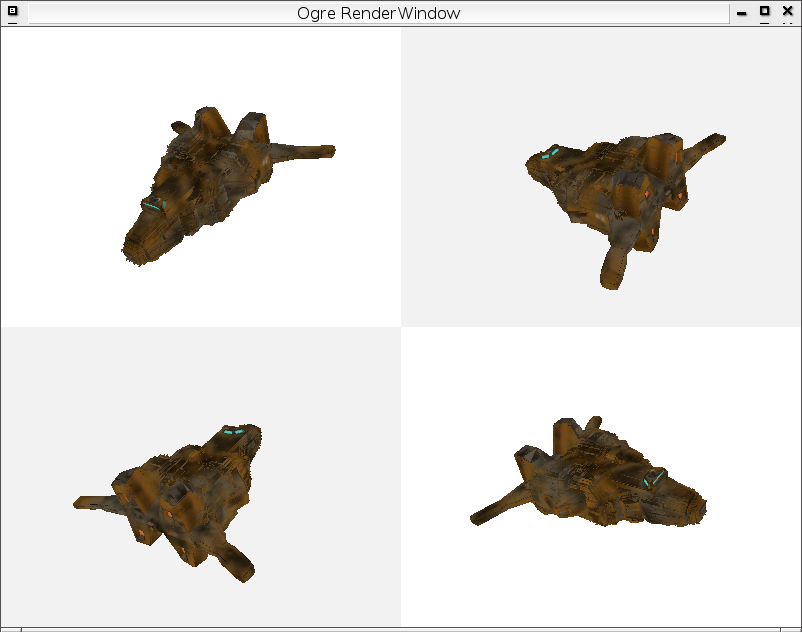
\includegraphics[width=8cm]{images/viewports/viewports.png}
		\caption{A render window displaying a single space ship in four different viewports.}
		\label{fig:ViewportExample}
	\end{figure}

	All our reference engines allow us to partition the render plane of the windows to create multiple smaller regions that each display the rendered output of one camera, as demonstrated by Figure \ref{fig:ViewportExample}. This approach allows developers to implement split-screen games, for example. All three engines provide this feature, although they all use different names for this fraction of the window displaying the output of a camera:

	\begin{smalllist}
		\item Ogre3d calls them \emph{Viewports},
		\item in Panda3d, these are \emph{DisplayRegions}, whereas
		\item OpenScenegraph refers to them as \emph{Views}.
	\end{smalllist}
	
	We will be using the term \classname{Viewport}, as this is the technical term for this construct and the other names do not provide any additional insight into this entity. Figure \ref{fig:WindowCameraAssociation} shows the general association between windows, viewports and cameras\footnote{A viewport is actually not limited to a single camera in all reference implementations, but we will stick to this simple model for our library.}. A viewport contains information on how the camera view is embedded into a window.

	\begin{figure}[htbp]
		\centering
		
\includegraphics[width=8cm]{images/OgreWindowViewport.png}
		\caption{Associations between windows, viewports and cameras.}
		\label{fig:WindowCameraAssociation}
	\end{figure}

	One important property a viewport needs is its \emph{z-index}. This value is consulted whenever viewports overlap. The one with the lower value is drawn first and is overlapped by the viewports ``above'' it.

	The implementation of these structures are described during the implementation of the \classname{Renderer} in Section \ref{chapter:implementation:renderer}.


	\section{Relative Orientation}
\label{chapter:design:coordinatesystem}

	The Cartesian \termdef{Coordinate System} of the 3-dimensional space of a scene has two properties that need to be defined in order to position objects therein:

	\begin{smalllist}
		\item Handedness: The direction the third vector points to, when the first two are defined.
		\item Orientation: The directions the three vectors point to relative to the render window.
	\end{smalllist}

	The orientation is unnecessary for the definition of the coordinate system from a mathematical point of view, since all orientations with the same handedness can be transformed to each other using a single rotation around the origin according to Euler's rotation theorem\cite{PP07}. But since human orientation rather happens in terms of relative directions -- up, down, left, right, forward, backward -- we will try to use these directions instead of the named axes $X$, $Y$ and $Z$.

	The lack of a standard mapping\footnote{OpenGL and Direct3D9 both use X/Y for left/up but differ in handedness, OpenGL defining negative Z as the forward vector\cite{Buss:2003:CGM:861813}, whereas Direct3D9 chooses positive Z\cite{jones2004beginning}. Panda3d, on the other hand, implements a right-handed coordinate system where X, Y and Z correspond to right, forward and upward\cite{Goslin:2004:PGE:1032275.1032359}.} is taken as an indicator that it is best left to personal preference. The choice will not have any effect on the API if orientation is expressed throughout the application, but it will still have two effects on the result:

	\begin{smalllist}
		\item If relative movement using the terms ``up'' or ``down'' are used alongside vectors for positioning objects, the three components of the vector will each map to one relative direction. There will be a visible difference between the exact same applications using different coordinate systems.
		\item The other implication is not so obvious: The underlying renderer will need to perform additional operations if the handedness of the coordinate systems differs from its own usage. We will elaborate on this effect during the implementation of the \classname{Renderer} in Section \ref{chapter:implementation:renderer}.
	\end{smalllist}

	Conceptually, the desired orientation serves but a single purpose: to assign a default rotation to newly created objects. All rotatable objects have a predefined orientation, or predefined directions that are considered that object's forward, right and up vectors. The orientation of the coordinate system rotates all new objects to align those directional vectors to those of the coordinate system's orientation. Figure \ref{fig:RotatedSpotLight} shows a newly created spot light that was positioned facing forward in the coordinate system orientation of Direct3D9 -- assuming that the forward orientation of a spot light is defined by the direction vector its light is emitted to.

	As long as the coordinate system to use during development is defined before any objects have been created, the library does not need to care about the coordinate system in use. We will need to define how the application behaves if the coordinate system is changed at run-time:

	Although it would technically be possible to re-position all objects within the scene, we have chosen to ignore this event. Although changing the coordinate system after having used it for positioning can lead to unexpected results, it is still possible to set the desired coordinate system at any point during run-time. The responsibility for choosing a system before starting the scene setup is left to the developer.
	
	Since changing the coordinate system of a project during development would lead to quite unexpected behavior, this constraint appears acceptable. We will be using the OpenGL standard as the default coordinate system in our library if no other system is set explicitly.

	\begin{figure}[htbp]
		\centering
		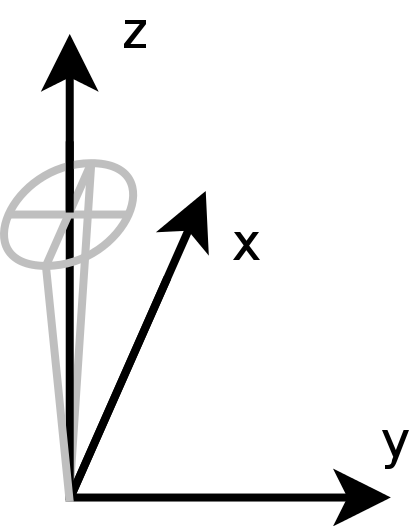
\includegraphics[width=4cm]{images/rotatedspotlight.png}
		\caption{A spot light facing ``forward'' in the Direct3D9 coordinate system, assuming its front-side is the direction the light is emitted to.}
		\label{fig:RotatedSpotLight}
	\end{figure}

	Although such relative axes are defined in all graphics engines, they are not an integral part of the API. The orientation serves a more technical purpose: When the scene is viewed from a certain point, every other object is positioned in a coordinate system that has its origin at that point. All objects left of the viewer have a negative $X$ value in OpenGL or Direct3D9 at this point. The mapping of named axes to the relative directions are only performed, as the whole scene is transformed into this coordinate system eventually.

	The orientation is still used as a default alignment of new objects but a ``rotation to the left'' does not exist in any of the reference APIs\footnote{Although Ogre3d provides equivalent methods called \inlinecode{yaw()}, \inlinecode{pitch()} and \inlinecode{roll()}, the wording is intentionally chosen \emph{not} to resemble orientation relative to the current position.}, rendering the original definition less useful than it could be. Whatever the orientation of the coordinate system is, one must fall back to the usage of the named coordinate axes $X$, $Y$ and $Z$ during application development.

	We will introduce relative orientation into the API to make stronger use of the already-present orientation capabilities of humans in the real world. If the Direct3D9 alignment of the coordinate system was chosen, a rotation around the $Y$ axis can be expressed as a rotation to the right: \inlinecode{rotateRight(Degree(90));}.

	A problem with an approach using this model is the ambiguity of the reference position. A very good example one is immediately confronted with when getting acquainted with a graphics library API is the rotation of a camera. We will start to explore this issue by defining three distinct axes along which one could perform rotations in our relative coordinate system. These axes reach
	
	\begin{smalllist}
		\item from left to right,
		\item from down to up and
		\item from backward to forward.
	\end{smalllist}

	The problem with cameras is that the human brain is not used to process tilted images. A camera that was rotated along the backward-forward axis tends to look odd, as demonstrated by Figure \ref{fig:TiltedCamera}. This means that the rotational axes for the default use of cameras can be reduced to two:
	
	\begin{figure}[htbp]
		\centering
		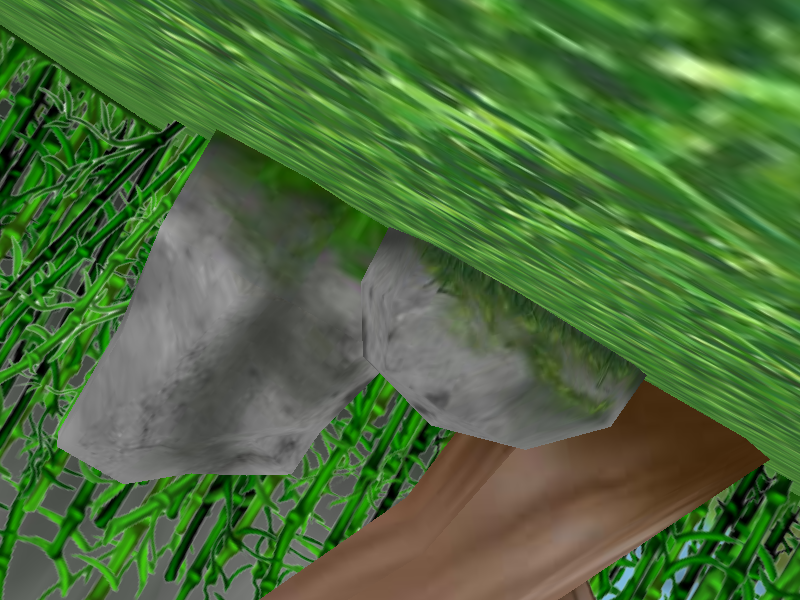
\includegraphics[width=14cm]{images/tiltedcamera/cam.png}
		\caption{A tilted camera}
		\label{fig:TiltedCamera}
	\end{figure}

	\begin{smalllist}
		\item from left to right (for looking up/down) and
		\item down to up (for looking to the sides).
	\end{smalllist}

	The next issue arises when these two axes are used consecutively. A camera that was rotated to look downward -- a rotation along the left-right axis -- a rotation along the down-up axis -- with the intention of looking sideways -- introduces an amount of tilt. This phenomenon is a result of the rotation along a local axis -- the tilt of the object has not changed from the viewpoint of the camera object itself, but the tilt of the current orientation of the camera has -- from the viewpoint of an unrotated scene node, as seen in Figure \ref{fig:CameraRotation}.

	\begin{figure}[htbp]
		\centering
		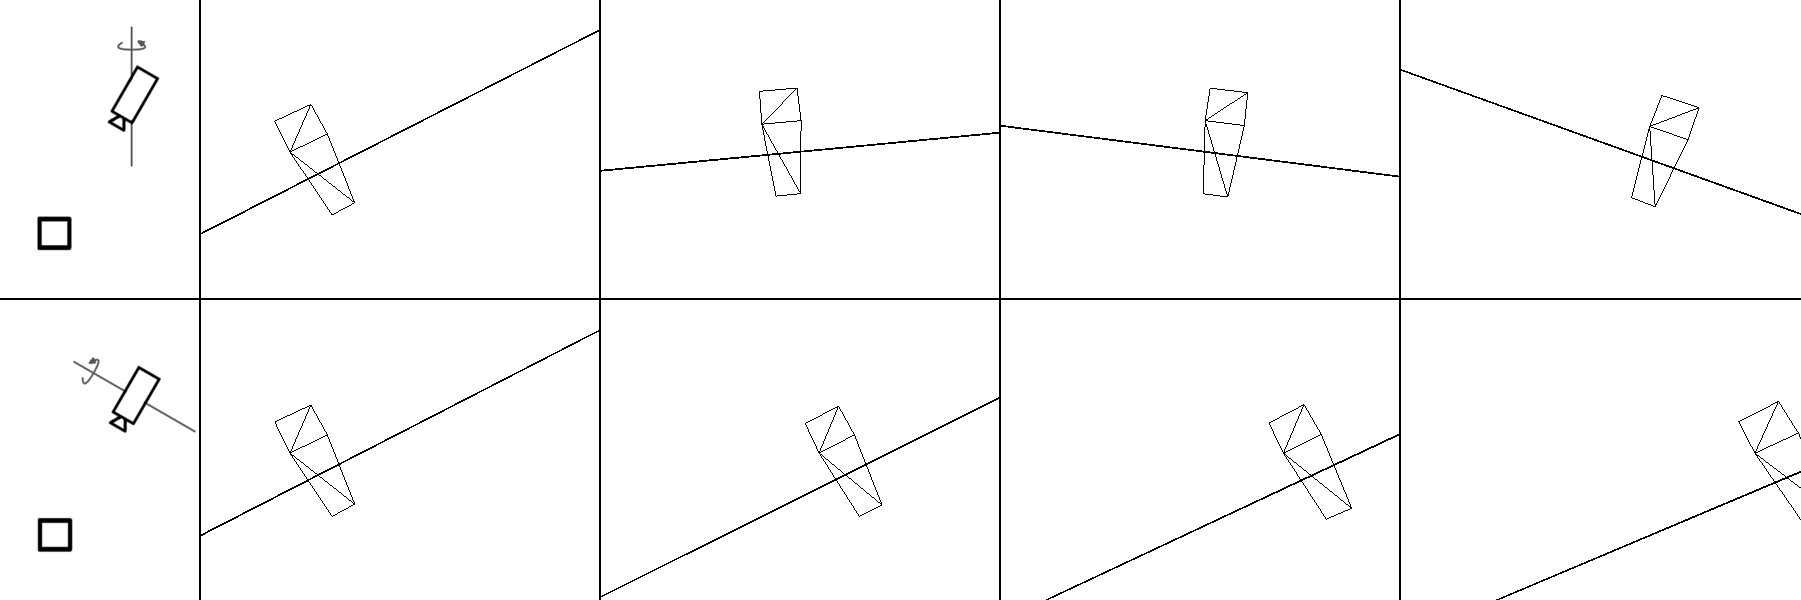
\includegraphics[width=14cm]{images/camera/camera.png}
		\caption{Rotating a camera looking down on a cube around the global coordinate system (upper frames) and its local coordinate system (lower frames). The lower images demonstrate that the tilt of the camera has not changed within its local coordinate system: the line on the floor is always parallel to that in other frames.}
		\label{fig:CameraRotation}
	\end{figure}

	The available rotation axes to a camera are further constrained to

	\begin{smalllist}
		\item the \emph{local} axis traversing from left to right and
		\item the \emph{global} axis pointing upwards.
	\end{smalllist}

	This example demonstrates the main issue with rotations. Every rotation consists of two distinct components:

	\begin{numlist}
		\item an axis/angle pair that defines the rotation and
		\item the coordinate system the rotation is to be performed in.
	\end{numlist}

	There are two approaches in our reference engines to the ambiguity arising due to the non-commutative nature of quaternion multiplication during rotations. Prior to these solutions, we must take note that all reference engines use quaternions for the orientation within the scene. The following is an example in Ogre3d:

	% leading whitespace in the following code snippet must consist of spaces, not tabs!
	\begin{code}[2]
		Quaternion rotation1;
		Quaternion rotation2;
		rotation1.FromAngleAxis(Degree(90), Vector3::UNIT_Y)
		rotation2.FromAngleAxis(Degree(90), Vector3::UNIT_X)
		sceneNode->rotate(rotation1 * rotation2);
	\end{code}

	The quaternions are used differently by our reference engines, though:

	\begin{smalllist}
		\item Ogre3d's \classname{SceneNode} has a method \inlinecode{rotate()} that accepts a quaternion as first, and the \classname{TransformSpace} as second parameter. The \classname{TransformSpace} is an enum consisting of the values
		\begin{smalllist}
			\item \inlinecode{TS\_LOCAL} -- rotation within the current orientation, this is the default value of this parameter
			\item \inlinecode{TS\_PARENT} -- rotation within the orientation of the parent scene node
			\item \inlinecode{TS\_WORLD} -- rotation from the viewpoint of an unrotated scene node
		\end{smalllist}
		\item The other libraries do not provide any means of rotating rotated nodes at all. The only option is to \emph{re-set} the orientation of a scene node. The developer is responsible for the creation of the desired quaternion for this purpose.
	\end{smalllist}

	Although Ogre3d uses three predefined context spaces, the rotation is not limited to those three, so we will approach the issue from a different angle. Instead of limiting the contexts to these values, we will declare that a rotation requires a \emph{context node} the operation is performed in. In the camera example above, this is either the parent node (casually referred to as ``local'' value above), or the root node of the scene graph (the ``global'' value).

	Every node should actually be viewed as a coordinate system that is embedded into another coordinate system\footnote{Except for the root node, which does not have a parent}. In other words: every child node creates a sub-space within its parent node. This means that the global result of a rotation will change depending on the space the query is performed in.

	%\begin{minipage}{15.35cm}
	\begin{code}[2]
		sceneNode->rotate(quaternion, context);
	\end{code}
	%\end{minipage}

	This choice brings up an ambiguity: it is not clear, whether the \inlinecode{context} implies an \emph{orientation} or a \emph{location}. The above code snippet could be interpreted as either of:

	\begin{smalllist}
		\item ``Perform the rotation as if the \inlinecode{context} node was looking at \inlinecode{sceneNode} from its current \emph{position}.''
		\item ``Perform the rotation as if the \inlinecode{context} node was re-positioned to look at \inlinecode{sceneNode} without changing its \emph{orientation}.''
	\end{smalllist}

	We have accepted this flaw and kept this solution, since the behavior during re-orientation is application-specific -- a camera would probably be rotated differently than an asteroid floating in space without gravity. Re-positioning a node leaves much less room for interpretation: the only remaining variable is the distance to the object, which is irrelevant for this purpose.

	The implementation of the concepts described here can be found in Section \ref{chapter:implementation:scenegraph}.


	\section{Scene Graph}
\label{chapter:implementation:scenegraph}

	The basic design of the base class for all specialized scene nodes is presented in Figure \ref{fig:SceneNode1}. Note that there are many more methods in the actual implementation that were only added for convenience. We will look at the implementation of all methods in this graph, dividing them into two categories:

	\begin{smalllist}
		\item Re-parenting
		\item Property Queries and Modifications
	\end{smalllist}

	We will additionally look into the implementation of some convenience methods and patterns that try to further simplify the API.

	\begin{figure}[htbp]
		\centering
		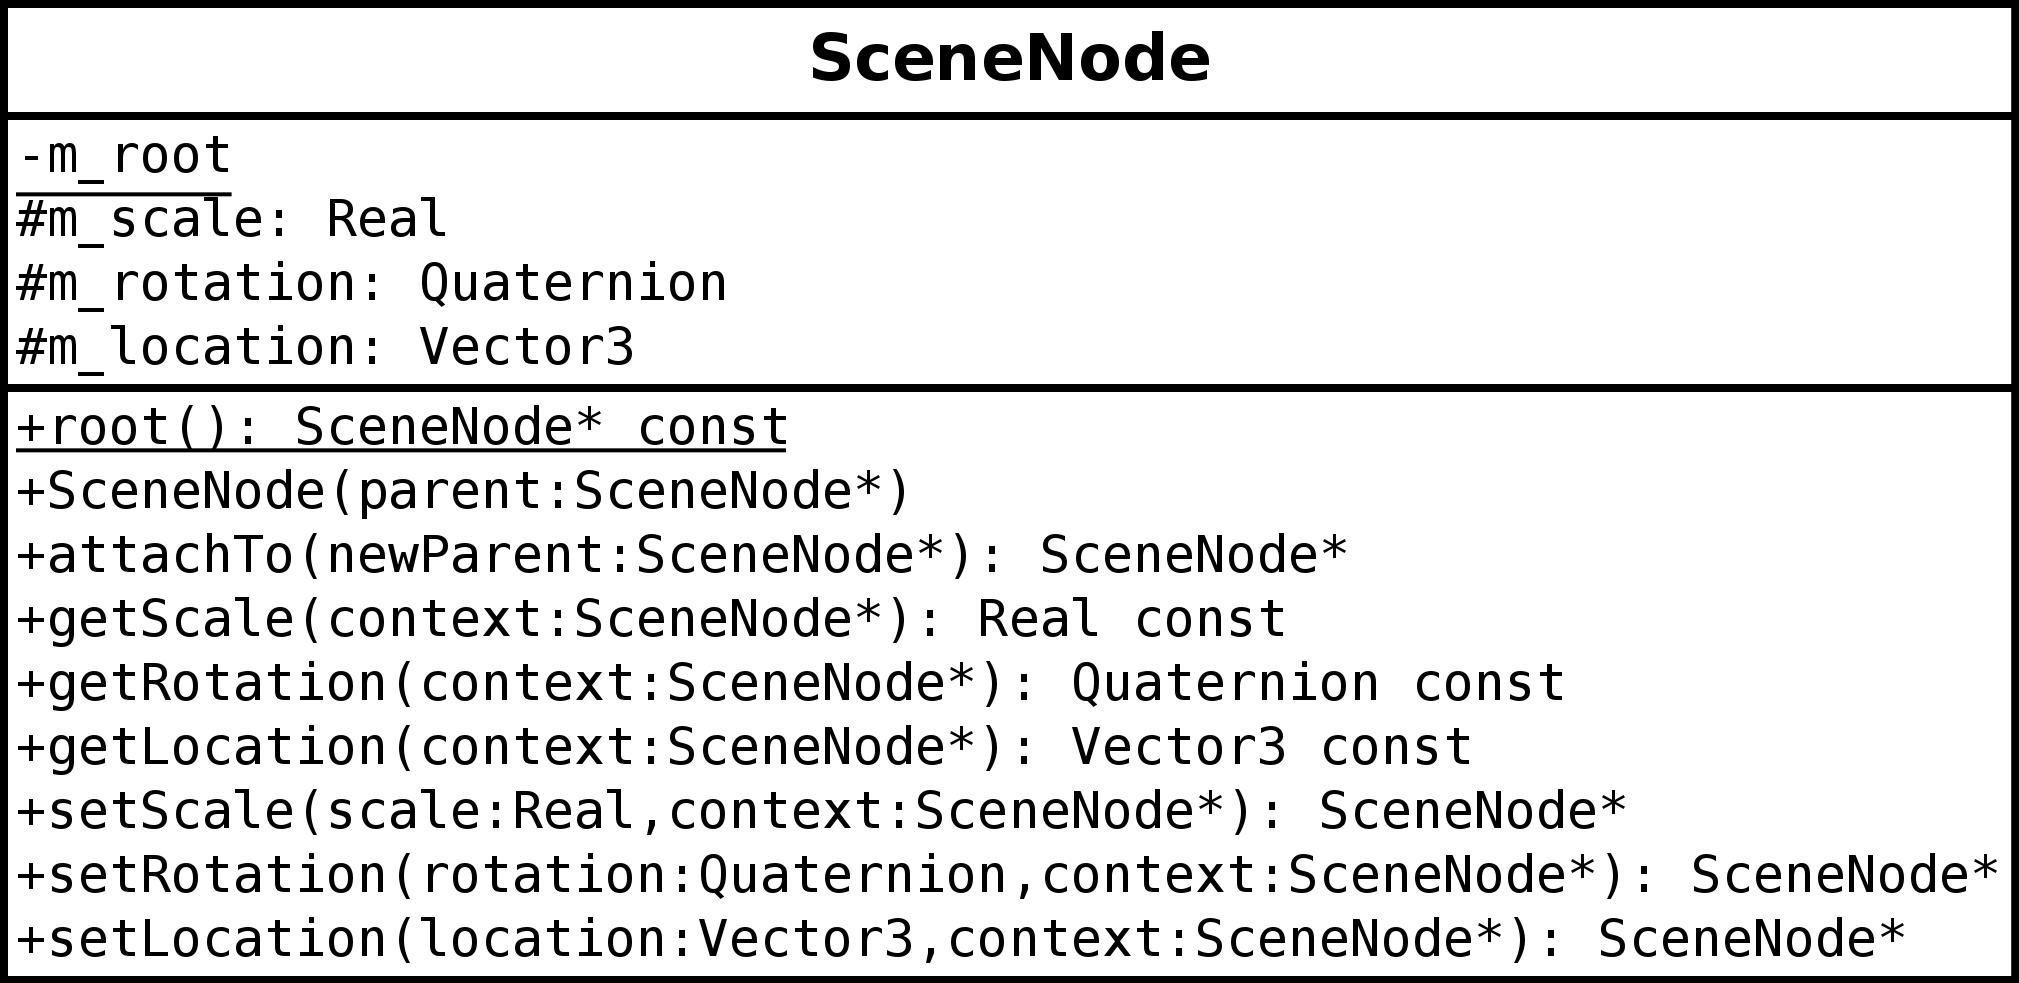
\includegraphics[width=10cm]{images/SceneNode1.png}
		\caption{Basic layout of the \classname{SceneNode} class.}
		\label{fig:SceneNode1}
	\end{figure}

	\subsection{Re-parenting}

		When arbitrary re-parenting of scene nodes is supported in an API, there is the possibility to create circular dependencies:

		\begin{code}[2]
			knifeNode->attachTo(forkNode);
			forkNode->attachTo(knifeNode);
		\end{code}

		We have three solutions to this issue: Either

		\begin{smalllist}
			\item the API is designed in a way that makes it impossible to create any circular dependencies,
			\item the issue is ignored altogether as such a circular construct is no longer part of the scene graph and does not have any impact on the visual output, or
			\item the library checks for them at certain points during the execution.
		\end{smalllist}

		The only available solution eliminating the problem altogether is the prohibition of re-parenting scene nodes. It is not possible to generate circular dependencies if an existing parent node is responsible for creating new nodes and those parents cannot be re-attached to other nodes. We will discard this very effective solution, as it renders the scene graph API very inflexible.

		The next option is to ignore such constructs. As every node has exactly one parent, a circle implies that it does not have a reference to the root scene node. Since the scene only contains nodes that are somehow attached to the root node, these nodes won't be displayed at all. This choice could lead to bugs that are quite hard to find for the same reason.

		The remaining option involves verifying the tree structure either when the scene graph changes or when the parent of a scene node is queried. Since the parent node is expected to change less often than it is queried, the check for circular references is performed immediately after an object is attached to another one. This choice additionally provides much more concise error messages and better supports debugging of such an error case.

	\subsection{Property Query and Modification}

		\subsubsection{Scale}

			The scale of a node in the global context is the product of all scale factors in all parent nodes: $s_g = s_{p_0} \cdot s_{p_1} \cdot \ldots \cdot s_{p_n} \cdot s_n$. Evaluating the scale of a scene node from the viewpoint of another node, we just need to find the quotient of the global scale values of the viewpoint and the queried node:

			\begin{code}[4]
				Real SceneNode::getScale(SceneNode* context) {
				    if (context == parent) {
				        return m_scale;
				    }
				    if (context == root()) {
				        return parent->getScale(root()) * m_scale;
				    }
				    return getScale(root()) / context->getScale(root());
				}
			\end{code}

			Although this implementation would be sufficient, we have added another dedicated if-block for handling the case where \inlinecode{context == this}, as the return value is always 1 in this case. Space never seems distorted from ones own viewpoint.
	
			After the implementation of the query method, the implementation of the setter becomes trivial:

			\begin{code}[4]
				SceneNode* SceneNode::setScale(Real s, SceneNode* context) {
				    m_scale *= s / getScale(context);
				    return this;
				}
			\end{code}

		\subsubsection{Rotation}

			Rotations are stored as a rotation within the coordinate system of the parent node. To evaluate the rotation of a scene node in the global context, we will need to multiply the rotations of all parent nodes. The return value of \inlinecode{node->getRotation(RootSceneNode::get())} is computed by $r_g = r_{p_0} \cdot r_{p_1} \cdot \ldots \cdot r_{p_n} \cdot r_n$, where $r_n$ denotes the rotation quaternion of the current node and $r_{p_0}$ through $r_{p_n}$ are the rotation quaternions of the parent nodes.

			To evaluate the rotation of a node in the coordinate system of another node, we can take the rotations of both nodes in the global coordinate system and compute the necessary quaternion that would change the rotation of the viewpoint to that of the target. If $r_g$ and $R_g$ are the global rotation quaternions of the target and context nodes respectively, the rotation from $R_g$ to $r_g$ can be computed using $\Delta r = R_g^{-1} \cdot r_g$.

			The resulting quaternion $\Delta r$ can be used to rotate $R_g$ to $r_g$, as $R_g \cdot \Delta r = R_g \cdot R_g^{-1} \cdot r_g = r_g$. Surprisingly the steps required for this computation do not differ from the evaluation of the scale. This defines the implementation of \inlinecode{getRotation()} method very similar to \inlinecode{getScale()}:

			\begin{code}[4]
				Quaternion SceneNode::getRotation(SceneNode* context) {
				    if (context == parent) {
				        return m_rotation;
				    }
				    if (context == root()) {
				        return parent->getRotation(root()) * m_rotation;
				    }
				    return context->getRotation(root()).inverse() *
			            getRotation(root());
				}
			\end{code}

			The method for updating the rotation is analogous to \inlinecode{setScale} as well:

			\begin{code}[4]
				SceneNode* SceneNode::setRotation(Quaternion r, SceneNode* context) {
				    Quaternion perceivedRot = getRotation(context);
				    m_rotation *= perceivedRot.inverse() * r * perceivedRot;
				    return this;
				}
			\end{code}

		\subsubsection{Location}

		Finding the location of an object is a bit more complex, as the calculation involves the other two properties. The position in global space is defined by \[l_g = l_{p_0} + (r_{p_0} \cdot l_{p_1} \cdot s_{p_0}) + \ldots + (r_{p_{n-1}} \cdot l_{p_n} \cdot s_{p_{n-1}}) + l_n\] This is necessary as the \emph{rotation} and \emph{scale} properties do not effect the node they have been defined in but solely effect the sub-space they are creating.

			This makes the calculation of a relative location to another more complex as well. After finding the global positions of both nodes (the queried node and the context node), we can create a vector pointing from one point to the other. We will need to adjust that vector using the rotation and scale of the own values of the context node: \[\Delta l = R_n \cdot (l_g - L_g) \cdot S_n\]

			After that we can use $\Delta l$ to position an object in the space of the context node at the exact same position as the initially queried node. The implementation of this method explicitly requires the handling of the context node being the parent node this time:

			\begin{code}[4]
				Vector3 SceneNode::getLocation(SceneNode* context) {
				    if (context == parent) {
				        return m_location;
				    }
				    if (context == root()) {
				        return parent->getLocation(root()) +
				               parent->m_rotation * m_location * parent->m_scale;
				    }
				    return getLocation(root()) - context->getLocation(root());
				}
			\end{code}

			Setting the location from an external viewpoint is as simple as the setter of the other two properties:
			
			\begin{code}[4]
				SceneNode* SceneNode::setLocation(Vector3 l, SceneNode* context) {
					m_location += l - getLocation(context);
				    return this;
				}
			\end{code}

	\subsection{Convenience}

		\subsubsection{Additional Methods}

			The methods presented at the beginning of this Section are completely sufficient to perform all available operations on \classname{SceneNode}s. Being limited to these few operations would render the API unnecessarily complex. We will try to hide any design details until the developer actively seeks them out. We have implemented a wide variety of additional methods for this purpose:

			\begin{smalllist}
				\item Property modification without context, where the context is assumed to be the parent node:
				\begin{smalllist}
					\item setScale(Real scale)
					\item setRotation(Quaternion rotation)
					\item setLocation(Vector3 location)
				\end{smalllist}
				\item Relative property modification:
				\begin{smalllist}
					\item scale(Real scalar)
					\item rotate(Quaternion rotation)
					\item move(Vector3 vector)
				\end{smalllist}
				\item Relative movement and rotation, both with and without the additional context parameter:
					\begin{smalllist}
						\item \begin{tabular}{|l}
								moveLeft(Real amount) \\ moveRight(Real amount)
							\end{tabular}
						\item \begin{tabular}{|l}
								moveUp(Real amount) \\ moveDown(Real amount)
							\end{tabular}
						\item \begin{tabular}{|l}
								moveForward(Real amount) \\ moveBackward(Real amount)
							\end{tabular}
						\item \begin{tabular}{|l}
								rotateLeft(Angle amount) \\ rotateRight(Angle amount) \\ turnLeft(Angle amount) \\ turnRight(Angle amount)
							\end{tabular}
						\item \begin{tabular}{|l}
								rotateUp(Angle amount) \\ rotateDown(Angle amount) \\ turnUp(Angle amount) \\ turnDown(Angle amount)
							\end{tabular}
						\item \begin{tabular}{|l}
								tiltLeft(Angle amount) \\ tiltRight(Angle amount)
							\end{tabular}
					\end{smalllist}
			\end{smalllist}

			The definition of these methods have bloated the API on one hand, but provided the perfect method for many use cases. We have noticed during testing that we were not using quaternions at all. We were able to create our test scenes just with relative modification of our objects.

		\subsubsection{Fluent Interfaces}

			When embedding an object into the scene graph, we need to adjust several properties of the object. Usually this involves multiple distinct calls to a newly created scene node. A pattern that we immediately thought of with this insight was the fluent interface\cite{Fowler2010}. Fluent interfaces return the object that is being operated on to allow us to chain multiple methods. The above example would be reduced to just four lines of code with the implementation of this idea:

			% whitespace
			\begin{code}[4]
				table = Model::create("Table");
				cutlery = SceneNode::create()
				    ->setPosition(1, 1, 10)
				    ->attachTo(table);
				knife = Model::create("Knife")
				    ->setPosition(1, 0, 0);
				    ->attachTo(cutlery);
				fork = Model::create("Fork")
				    ->attachTo(cutlery);
			\end{code}

			Unfortunately, we had chosen to sub-class the \classname{SceneNode} for each object type that can be attached to the scene graph. This means that any operation on the \classname{SceneNode} API would return a \classname{SceneNode} object and no longer its sub-class. But a fluent API returning the covariant type would be much more intuitive to avoid the following scenario:
			
			% whitespace
			\begin{code}[4]
				light = SpotLight::create()
				    // the next call would return a SceneNode object
				    // which does not provide the setColor() method:
				    ->setPosition(1, 1, 1)
				    // compilation error on the next line:
				    ->setColor(Color::RED);
			\end{code}

			The simplest solution would be to re-implement all methods of the \classname{SceneNode} in the \classname{SpotLightNode} class to return the type of the implementing class. Instead of performing this implementation in each sub-class of \classname{SceneNode}, we will use the \emph{curiously recurring template pattern} (CRTP) to accomplish this task. \cite{Lippman:1996:CG:260627} presents this pattern based on work in \cite{Barton:1994:SEC:561392} and its implementation in our library is presented in Figure \ref{fig:FluentInterface}

			\begin{figure}[htbp]
				\centering
				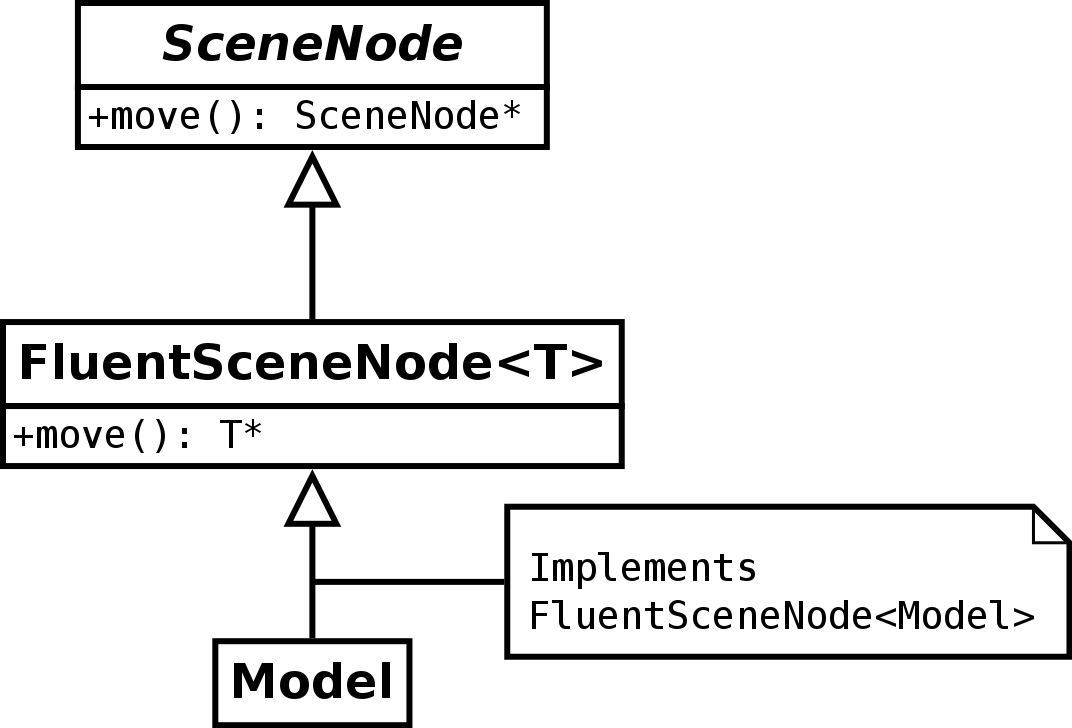
\includegraphics[width=8cm]{images/FluentInterface.png}
				\caption{The architecture of the fluent interface. The template class' method \inlinecode{FluentSceneNode<T>::move()} executes \inlinecode{SceneNode::move()} and returns \inlinecode{this}, casting it to a \inlinecode{T} pointer.}
				\label{fig:FluentInterface}
			\end{figure}

			The API now returns the type of the object an operation was called on, allowing us to use all methods of a \classname{SpotLightNode} in succession, regardless of the implementation of the methods within the class hierarchy.


	\section{Scene Modification}

	When modifying the structure of a scene graph, the objects within the scene are modified implicitly. If a scene node is re-parented to another node, the properties of the child node change. If we consider the example in Figure \ref{fig:SceneNodeReparenting1}, the \inlinecode{getLocation()} method of the \classname{Child} node will return a different value after the re-parenting.

	\begin{figure}[htbp]
		\centering
		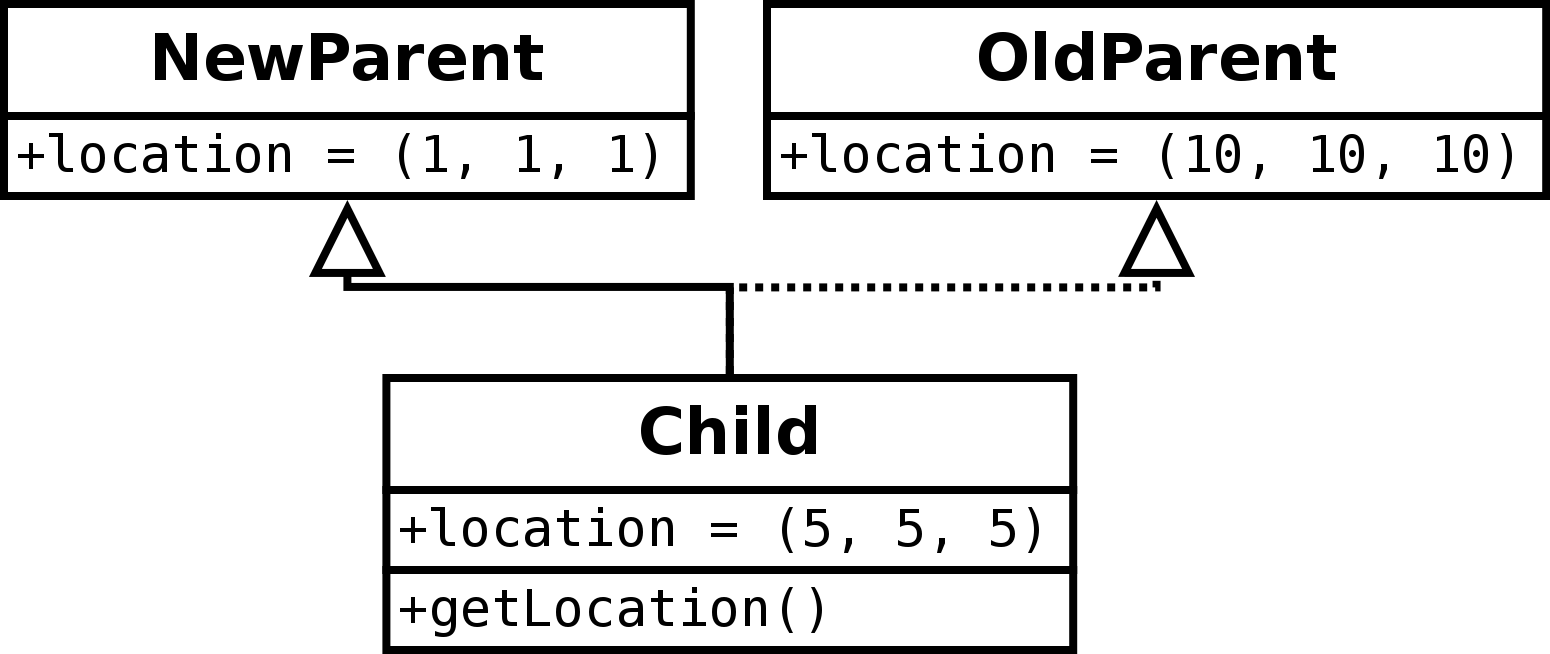
\includegraphics[width=6cm]{images/SceneNodeReparenting1.png}
		\caption{Example scene node re-parenting.}
		\label{fig:SceneNodeReparenting1}
	\end{figure}

	An object that has a \inlinecode{location} value of \vect{5}{5}{5} is positioned with that value as offset from the origin of its parent, no matter where the parent is positioned within the scene. The same is true for other properties of a scene node: rotating the \classname{TableNode} rotates all objects, updating the scale value propagates as well.

	The API needs to provide the means of keeping its property on a global scale. The object should be able to keep its location from the viewpoint of an observing camera, otherwise it will jump to another position in-between two frames. As none of our reference engines supports this operation, we will have to find a new solution.
	
	The adjustment of the object's properties is trivial from a mathematical stand point, so we could just allow the developer to pass the properties he/she wants to keep on a global scale as a parameter:

	\begin{code}[2]
		child->attachTo(newParent, POSITION | ORIENTATION);
	\end{code}

	But we had a similar problem during the design of relative rotations in Section \ref{chapter:design:coordinatesystem}. The choice at that point was to support passing arbitrary nodes as a point of reference, not limiting the developer to a set of predefined values. We will try to provide the same flexibility for this operation.

	Updating the property of a scene node while retaining its value relative to another node can be performed with these two steps:

	\begin{smalllist}
		\item The property value is queried from the viewpoint of the \emph{context node} before the object is detached from its \classname{OldParent}.
		\item The value is recalculated to match the previously queried value in the same context after the parent was changed.
	\end{smalllist}

	Finding a solution to these two operations is the foundation of the solution to the initial problem. We had already addressed the second operation in our previous discussion on relative orientation. The other operation could be performed on the same basis, leaving us with the following code sample:
	
	\begin{code}[2]
		location = child->getLocation(context);
		child->attachTo(newParent);
		child->setLocation(location, context);
	\end{code}

	We can further create a facade that updates all properties of the child node to match its previous values from the viewpoint of a context node:

	\begin{code}[2]
		child->attachTo(newParent, context);
	\end{code}

	Apart from the issues during re-arrangement of the scene graph, we will tackle another aspect of the API. We had discussed the possibility to register \classname{Task}s to be performed during the render cycle. We found that one usage scenario when getting familiar with a graphics API was the movement of objects. We were creating a separate class for updating the location of an object along a vector in each application for testing a graphics library.

	We decided to implement a dedicated \classname{Task} for this use case, as this is the most elementary form of scene modification over time. But instead of limiting the class to this single operation (movement in a single direction), we will be implementing all basic operations -- movement, rotation and scaling.

	These thoughts have led us to the design of the \classname{SceneNodeModificationTask}, which has the exact same interface as a \classname{SceneNode}. A basic class outline is shown by Figure \ref{fig:SceneNodeModificationTask}. An object of this type performs the operation repeatedly on an object as long as it is present in the main task group.

	\begin{figure}[htbp]
		\centering
		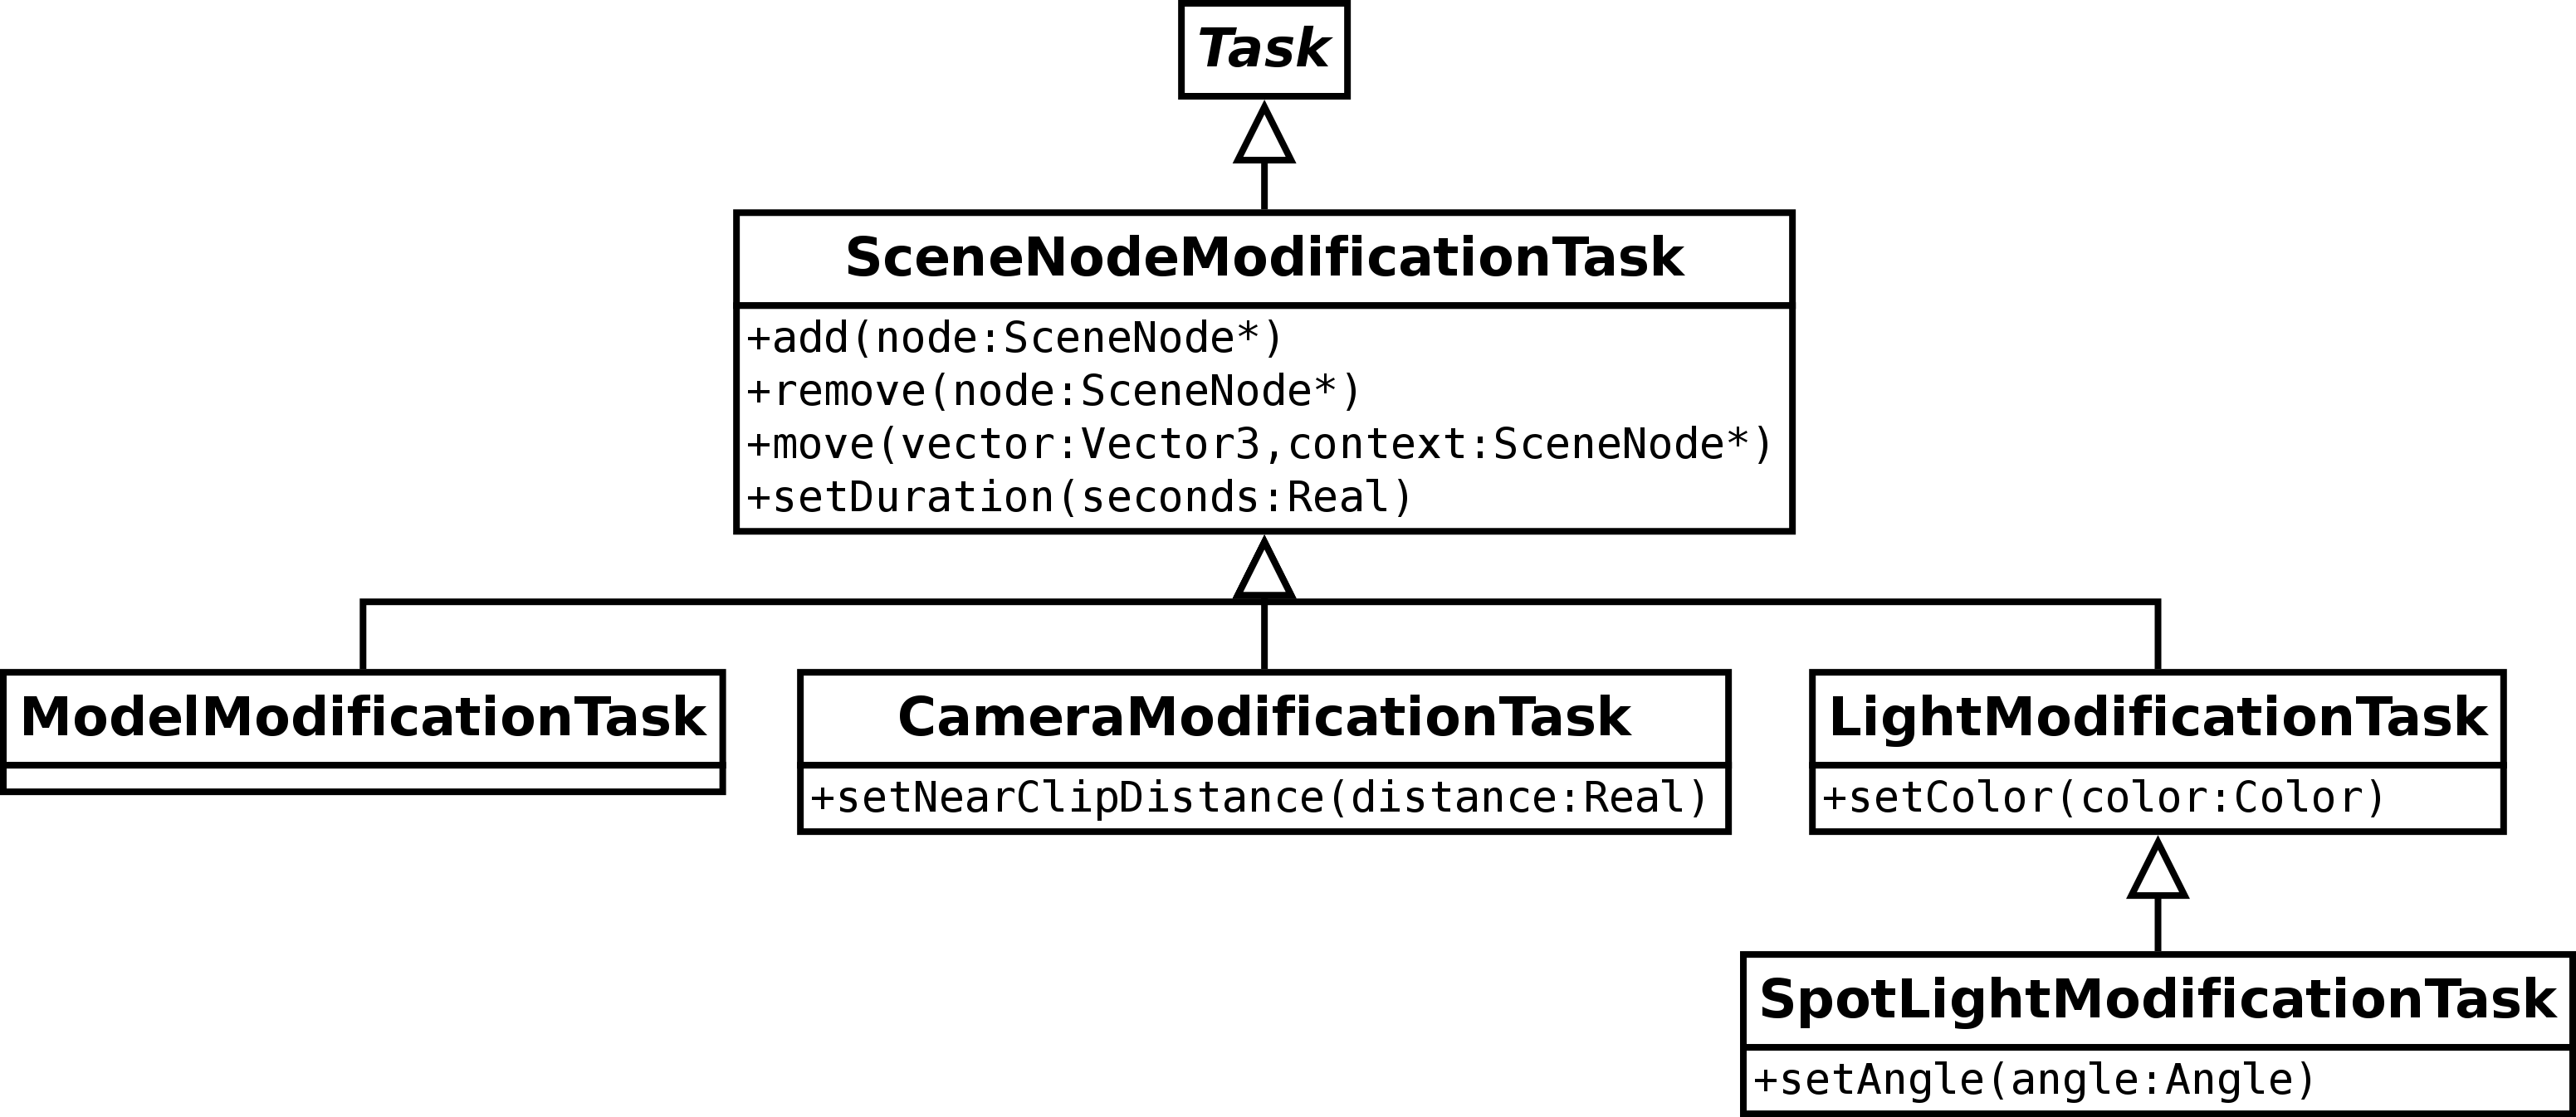
\includegraphics[width=14cm]{images/SceneNodeModificationTask.png}
		\caption{Outline of the \classname{SceneNodeModificationTask} classes. Note that the classes lack several methods that would unnecessarily clutter the diagram.}
		\label{fig:SceneNodeModificationTask}
	\end{figure}

	To configure the movement of an object along a vector, one needs to provide the vector at the length of the desired distance the object shall travel \emph{per second}. Implementing an object moving at a speed of 100 along the vector \vect{1}{1}{1} can be accomplished by the following code snippet:

	\begin{code}[2]
		task = ModelModificationTask::create();
		task->moveForward(Vector3(1, 1, 1).resize(100));
		task->register(model);
		MainTaskGroup::get()->add(task);
	\end{code}

	This \classname{Task} object will now repeatedly call the \inlinecode{moveForward()} method on the \inlinecode{model} at each loop cycle. The parameter vector will be re-sized during each call to have the correct length in relation to the time passed since its last call. The same procedure can be performed with rotations as well as scalars.

	The same concept can be applied to other properties of other objects. Dimming a spot light over the course of two seconds can be achieved with the following code:

	\begin{code}[2]
		task = LightModificationTask::create();
		task->setColor(Color::BLACK);
		task->setDuration(2);
		task->register(spotLight);
		MainTaskGroup::get()->add(task);
	\end{code}

	The implementation of these concepts are further described in Section \ref{chapter:implementation:scenegraph}.


	\chapter{Implementation}
	\section{General Information}

This document is intended as a template and guideline and should support the author in the course of doing the master's thesis.
Assessment criteria comprise the quality of the theoretical and/or practical work as well as structure, content and wording of the written master's thesis. Careful attention should be given to the basics of scientific work (e.g., correct citation).

\section{Organizational Issues}

A master's thesis at the Faculty of Informatics has to be finished within six months. During this period regular meetings between the advisor(s) and the author have to take place.
In addition, the following milestones have to be fulfilled:
\begin{enumerate}
  \item  Within one month after having fixed the topic of the thesis the master's thesis proposal has to be prepared and must be accepted by the advisor(s). The master's thesis proposal must follow the respective template of the dean of academic affairs. Thereafter the proposal has to be applied for at the deanery. The necessary forms may be found on the web site of the Faculty of Informatics. \url{http://www.informatik.tuwien.ac.at/dekanat/formulare.html}
  \item  Accompanied with the master's thesis proposal, the structure of the thesis in terms of a table of contents has to be provided.
  \item Then, the first talk has to be given at the so-called ``Seminar for Master Students''. The slides have to be discussed with the advisor(s) one week in advance. Attendance of the ``Seminar for Master Students'' is compulsory and offers the opportunity to discuss arising problems among other master students.
  \item At the latest five months after the beginning, a provisional final version of the thesis has to be handed over to the advisor(s).  
  \item As soon as the provisional final version exists, a first poster draft has to be made. The making of a poster is a compulsory part of the ``Seminar for Master Students'' for all master studies at the Faculty of Informatics. Drafts and design guidelines can be found at \url{http://www.informatik.tuwien.ac.at/studium/richtlinien}.
  \item After having consulted the advisor(s) the second talk has to be held at the ``Seminar for Master Students''.
  \item At the latest six months after the beginning, the corrected version of the master's thesis and the poster have to be handed over to the advisor(s).
  \item After completion the master's thesis has to be presented at the ``epilog''. For detailed information on the epilog see: \\ \url{http://www.informatik.tuwien.ac.at/studium/epilog}
\end{enumerate}

\section{Structure of the Master's Thesis}

If the curriculum regulates the language of the master's thesis to be English (like for ``Business Informatics''), the thesis has to be written in English. Otherwise, the master's thesis may be written in English or in German. The structure of the thesis is predetermined.
The table of contents is followed by the introduction and the main part, which can vary according to the content. The master's thesis ends with the bibliography (compulsory) and the appendix (optional).

\begin{itemize}
  \item	Cover page
  \item Acknowledgements
  \item Abstract of the thesis in English and German
  \item Table of contents
  \item Introduction
  	\begin{itemize}
  		\item motivation
  		\item problem statement (which problem should be solved?)
  		\item aim of the work
  		\item methodological approach
  		\item structure of the work
  	\end{itemize}
  \item State of the art / analysis of existing approaches
  	\begin{itemize}
  		\item literature studies
  		\item analysis
  		\item comparison and summary of existing approaches
  	\end{itemize}
  \item Methodology
  	\begin{itemize}
  		\item used concepts
  		\item methods and/or models
  		\item languages
  		\item design methods
  		\item data models
  		\item analysis methods
  		\item formalisms
  	\end{itemize}
  \item Suggested solution/implementation
  \item Critical reflection
  	\begin{itemize}
  		\item comparison with related work
  		\item discussion of open issues
  	\end{itemize}
  \item Summary and future work
  \item Appendix: source code, data models, \dots
  \item Bibliography
\end{itemize}


	\section{Scene Graph}
\label{chapter:implementation:scenegraph}

	The basic design of the base class for all specialized scene nodes is presented in Figure \ref{fig:SceneNode1}. Note that there are many more methods in the actual implementation that were only added for convenience. We will look at the implementation of all methods in this graph, dividing them into two categories:

	\begin{smalllist}
		\item Re-parenting
		\item Property Queries and Modifications
	\end{smalllist}

	We will additionally look into the implementation of some convenience methods and patterns that try to further simplify the API.

	\begin{figure}[htbp]
		\centering
		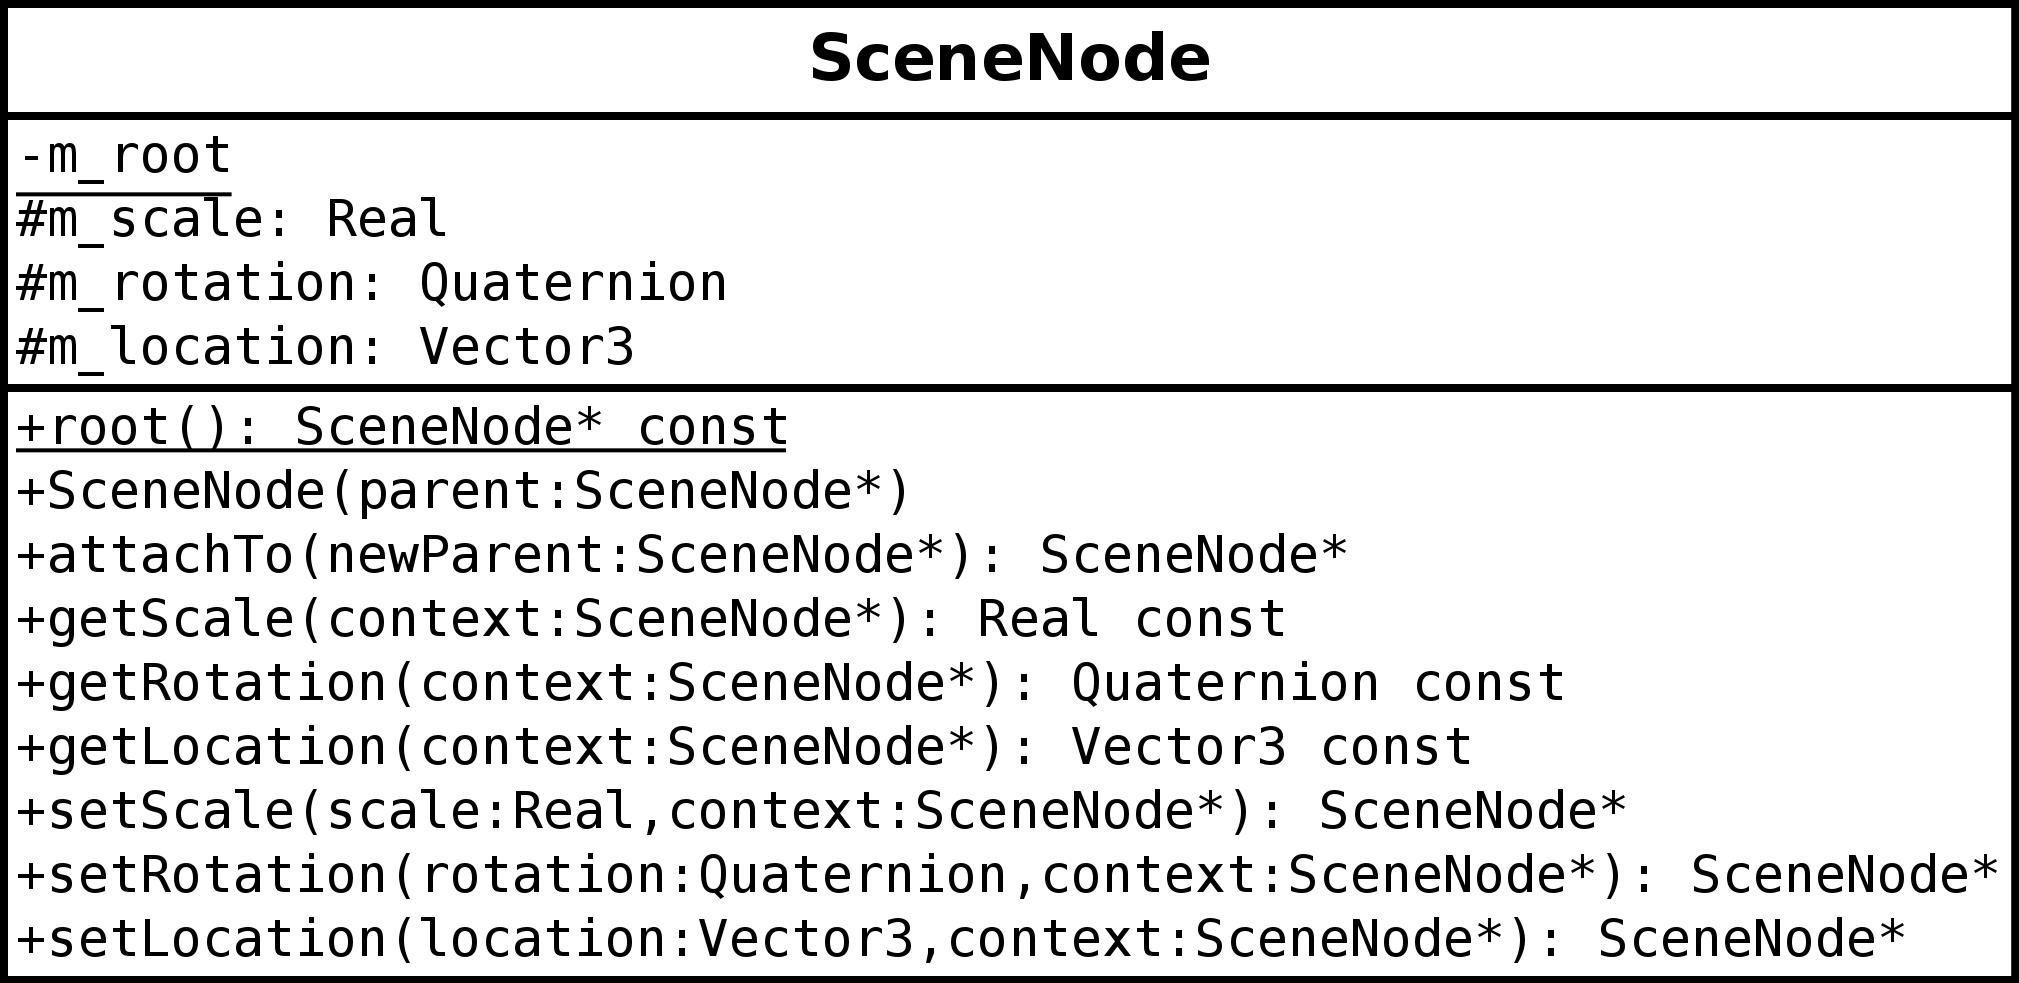
\includegraphics[width=10cm]{images/SceneNode1.png}
		\caption{Basic layout of the \classname{SceneNode} class.}
		\label{fig:SceneNode1}
	\end{figure}

	\subsection{Re-parenting}

		When arbitrary re-parenting of scene nodes is supported in an API, there is the possibility to create circular dependencies:

		\begin{code}[2]
			knifeNode->attachTo(forkNode);
			forkNode->attachTo(knifeNode);
		\end{code}

		We have three solutions to this issue: Either

		\begin{smalllist}
			\item the API is designed in a way that makes it impossible to create any circular dependencies,
			\item the issue is ignored altogether as such a circular construct is no longer part of the scene graph and does not have any impact on the visual output, or
			\item the library checks for them at certain points during the execution.
		\end{smalllist}

		The only available solution eliminating the problem altogether is the prohibition of re-parenting scene nodes. It is not possible to generate circular dependencies if an existing parent node is responsible for creating new nodes and those parents cannot be re-attached to other nodes. We will discard this very effective solution, as it renders the scene graph API very inflexible.

		The next option is to ignore such constructs. As every node has exactly one parent, a circle implies that it does not have a reference to the root scene node. Since the scene only contains nodes that are somehow attached to the root node, these nodes won't be displayed at all. This choice could lead to bugs that are quite hard to find for the same reason.

		The remaining option involves verifying the tree structure either when the scene graph changes or when the parent of a scene node is queried. Since the parent node is expected to change less often than it is queried, the check for circular references is performed immediately after an object is attached to another one. This choice additionally provides much more concise error messages and better supports debugging of such an error case.

	\subsection{Property Query and Modification}

		\subsubsection{Scale}

			The scale of a node in the global context is the product of all scale factors in all parent nodes: $s_g = s_{p_0} \cdot s_{p_1} \cdot \ldots \cdot s_{p_n} \cdot s_n$. Evaluating the scale of a scene node from the viewpoint of another node, we just need to find the quotient of the global scale values of the viewpoint and the queried node:

			\begin{code}[4]
				Real SceneNode::getScale(SceneNode* context) {
				    if (context == parent) {
				        return m_scale;
				    }
				    if (context == root()) {
				        return parent->getScale(root()) * m_scale;
				    }
				    return getScale(root()) / context->getScale(root());
				}
			\end{code}

			Although this implementation would be sufficient, we have added another dedicated if-block for handling the case where \inlinecode{context == this}, as the return value is always 1 in this case. Space never seems distorted from ones own viewpoint.
	
			After the implementation of the query method, the implementation of the setter becomes trivial:

			\begin{code}[4]
				SceneNode* SceneNode::setScale(Real s, SceneNode* context) {
				    m_scale *= s / getScale(context);
				    return this;
				}
			\end{code}

		\subsubsection{Rotation}

			Rotations are stored as a rotation within the coordinate system of the parent node. To evaluate the rotation of a scene node in the global context, we will need to multiply the rotations of all parent nodes. The return value of \inlinecode{node->getRotation(RootSceneNode::get())} is computed by $r_g = r_{p_0} \cdot r_{p_1} \cdot \ldots \cdot r_{p_n} \cdot r_n$, where $r_n$ denotes the rotation quaternion of the current node and $r_{p_0}$ through $r_{p_n}$ are the rotation quaternions of the parent nodes.

			To evaluate the rotation of a node in the coordinate system of another node, we can take the rotations of both nodes in the global coordinate system and compute the necessary quaternion that would change the rotation of the viewpoint to that of the target. If $r_g$ and $R_g$ are the global rotation quaternions of the target and context nodes respectively, the rotation from $R_g$ to $r_g$ can be computed using $\Delta r = R_g^{-1} \cdot r_g$.

			The resulting quaternion $\Delta r$ can be used to rotate $R_g$ to $r_g$, as $R_g \cdot \Delta r = R_g \cdot R_g^{-1} \cdot r_g = r_g$. Surprisingly the steps required for this computation do not differ from the evaluation of the scale. This defines the implementation of \inlinecode{getRotation()} method very similar to \inlinecode{getScale()}:

			\begin{code}[4]
				Quaternion SceneNode::getRotation(SceneNode* context) {
				    if (context == parent) {
				        return m_rotation;
				    }
				    if (context == root()) {
				        return parent->getRotation(root()) * m_rotation;
				    }
				    return context->getRotation(root()).inverse() *
			            getRotation(root());
				}
			\end{code}

			The method for updating the rotation is analogous to \inlinecode{setScale} as well:

			\begin{code}[4]
				SceneNode* SceneNode::setRotation(Quaternion r, SceneNode* context) {
				    Quaternion perceivedRot = getRotation(context);
				    m_rotation *= perceivedRot.inverse() * r * perceivedRot;
				    return this;
				}
			\end{code}

		\subsubsection{Location}

		Finding the location of an object is a bit more complex, as the calculation involves the other two properties. The position in global space is defined by \[l_g = l_{p_0} + (r_{p_0} \cdot l_{p_1} \cdot s_{p_0}) + \ldots + (r_{p_{n-1}} \cdot l_{p_n} \cdot s_{p_{n-1}}) + l_n\] This is necessary as the \emph{rotation} and \emph{scale} properties do not effect the node they have been defined in but solely effect the sub-space they are creating.

			This makes the calculation of a relative location to another more complex as well. After finding the global positions of both nodes (the queried node and the context node), we can create a vector pointing from one point to the other. We will need to adjust that vector using the rotation and scale of the own values of the context node: \[\Delta l = R_n \cdot (l_g - L_g) \cdot S_n\]

			After that we can use $\Delta l$ to position an object in the space of the context node at the exact same position as the initially queried node. The implementation of this method explicitly requires the handling of the context node being the parent node this time:

			\begin{code}[4]
				Vector3 SceneNode::getLocation(SceneNode* context) {
				    if (context == parent) {
				        return m_location;
				    }
				    if (context == root()) {
				        return parent->getLocation(root()) +
				               parent->m_rotation * m_location * parent->m_scale;
				    }
				    return getLocation(root()) - context->getLocation(root());
				}
			\end{code}

			Setting the location from an external viewpoint is as simple as the setter of the other two properties:
			
			\begin{code}[4]
				SceneNode* SceneNode::setLocation(Vector3 l, SceneNode* context) {
					m_location += l - getLocation(context);
				    return this;
				}
			\end{code}

	\subsection{Convenience}

		\subsubsection{Additional Methods}

			The methods presented at the beginning of this Section are completely sufficient to perform all available operations on \classname{SceneNode}s. Being limited to these few operations would render the API unnecessarily complex. We will try to hide any design details until the developer actively seeks them out. We have implemented a wide variety of additional methods for this purpose:

			\begin{smalllist}
				\item Property modification without context, where the context is assumed to be the parent node:
				\begin{smalllist}
					\item setScale(Real scale)
					\item setRotation(Quaternion rotation)
					\item setLocation(Vector3 location)
				\end{smalllist}
				\item Relative property modification:
				\begin{smalllist}
					\item scale(Real scalar)
					\item rotate(Quaternion rotation)
					\item move(Vector3 vector)
				\end{smalllist}
				\item Relative movement and rotation, both with and without the additional context parameter:
					\begin{smalllist}
						\item \begin{tabular}{|l}
								moveLeft(Real amount) \\ moveRight(Real amount)
							\end{tabular}
						\item \begin{tabular}{|l}
								moveUp(Real amount) \\ moveDown(Real amount)
							\end{tabular}
						\item \begin{tabular}{|l}
								moveForward(Real amount) \\ moveBackward(Real amount)
							\end{tabular}
						\item \begin{tabular}{|l}
								rotateLeft(Angle amount) \\ rotateRight(Angle amount) \\ turnLeft(Angle amount) \\ turnRight(Angle amount)
							\end{tabular}
						\item \begin{tabular}{|l}
								rotateUp(Angle amount) \\ rotateDown(Angle amount) \\ turnUp(Angle amount) \\ turnDown(Angle amount)
							\end{tabular}
						\item \begin{tabular}{|l}
								tiltLeft(Angle amount) \\ tiltRight(Angle amount)
							\end{tabular}
					\end{smalllist}
			\end{smalllist}

			The definition of these methods have bloated the API on one hand, but provided the perfect method for many use cases. We have noticed during testing that we were not using quaternions at all. We were able to create our test scenes just with relative modification of our objects.

		\subsubsection{Fluent Interfaces}

			When embedding an object into the scene graph, we need to adjust several properties of the object. Usually this involves multiple distinct calls to a newly created scene node. A pattern that we immediately thought of with this insight was the fluent interface\cite{Fowler2010}. Fluent interfaces return the object that is being operated on to allow us to chain multiple methods. The above example would be reduced to just four lines of code with the implementation of this idea:

			% whitespace
			\begin{code}[4]
				table = Model::create("Table");
				cutlery = SceneNode::create()
				    ->setPosition(1, 1, 10)
				    ->attachTo(table);
				knife = Model::create("Knife")
				    ->setPosition(1, 0, 0);
				    ->attachTo(cutlery);
				fork = Model::create("Fork")
				    ->attachTo(cutlery);
			\end{code}

			Unfortunately, we had chosen to sub-class the \classname{SceneNode} for each object type that can be attached to the scene graph. This means that any operation on the \classname{SceneNode} API would return a \classname{SceneNode} object and no longer its sub-class. But a fluent API returning the covariant type would be much more intuitive to avoid the following scenario:
			
			% whitespace
			\begin{code}[4]
				light = SpotLight::create()
				    // the next call would return a SceneNode object
				    // which does not provide the setColor() method:
				    ->setPosition(1, 1, 1)
				    // compilation error on the next line:
				    ->setColor(Color::RED);
			\end{code}

			The simplest solution would be to re-implement all methods of the \classname{SceneNode} in the \classname{SpotLightNode} class to return the type of the implementing class. Instead of performing this implementation in each sub-class of \classname{SceneNode}, we will use the \emph{curiously recurring template pattern} (CRTP) to accomplish this task. \cite{Lippman:1996:CG:260627} presents this pattern based on work in \cite{Barton:1994:SEC:561392} and its implementation in our library is presented in Figure \ref{fig:FluentInterface}

			\begin{figure}[htbp]
				\centering
				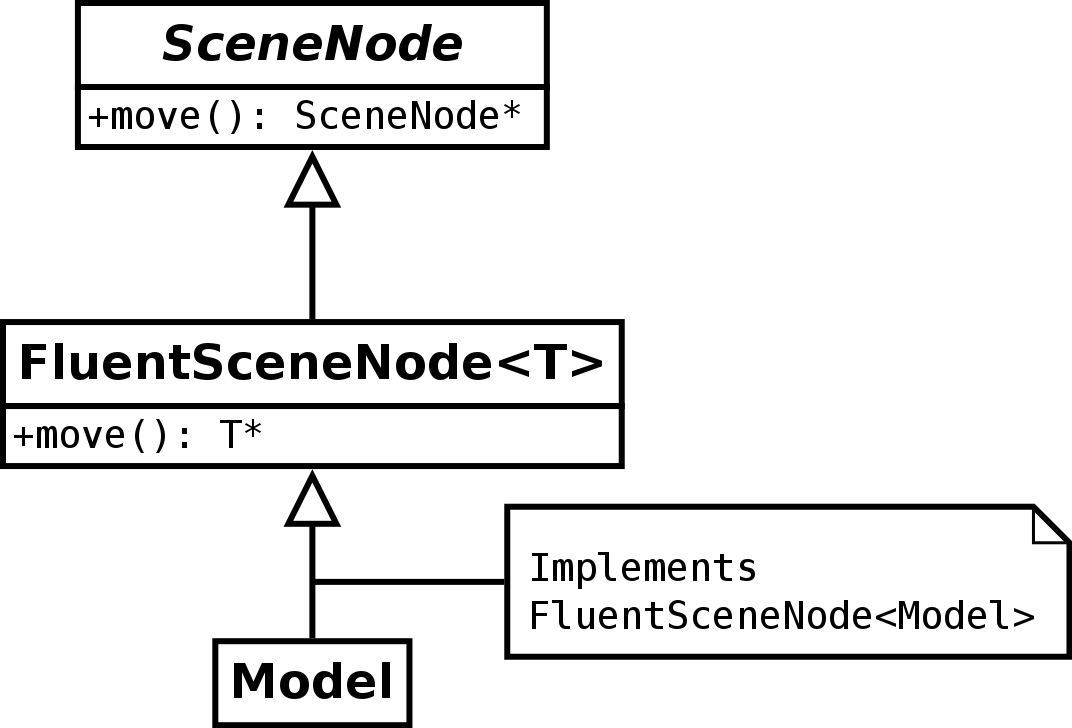
\includegraphics[width=8cm]{images/FluentInterface.png}
				\caption{The architecture of the fluent interface. The template class' method \inlinecode{FluentSceneNode<T>::move()} executes \inlinecode{SceneNode::move()} and returns \inlinecode{this}, casting it to a \inlinecode{T} pointer.}
				\label{fig:FluentInterface}
			\end{figure}

			The API now returns the type of the object an operation was called on, allowing us to use all methods of a \classname{SpotLightNode} in succession, regardless of the implementation of the methods within the class hierarchy.


	\section{External Renderer}
\label{chapter:design:renderer}

	Luckily, the usage of an external renderer already provides access to an advanced API. Users knowledgeable about the external graphics engine being used can fine-tune operations within that engine. Any object controlling the rendering process is created within the PURGE namespace, and adopted by the external rendering facility, the \classname{Renderer}. That facility is responsible for taking that object into account during the rendering process.

	\begin{figure}[htbp]
		\centering
		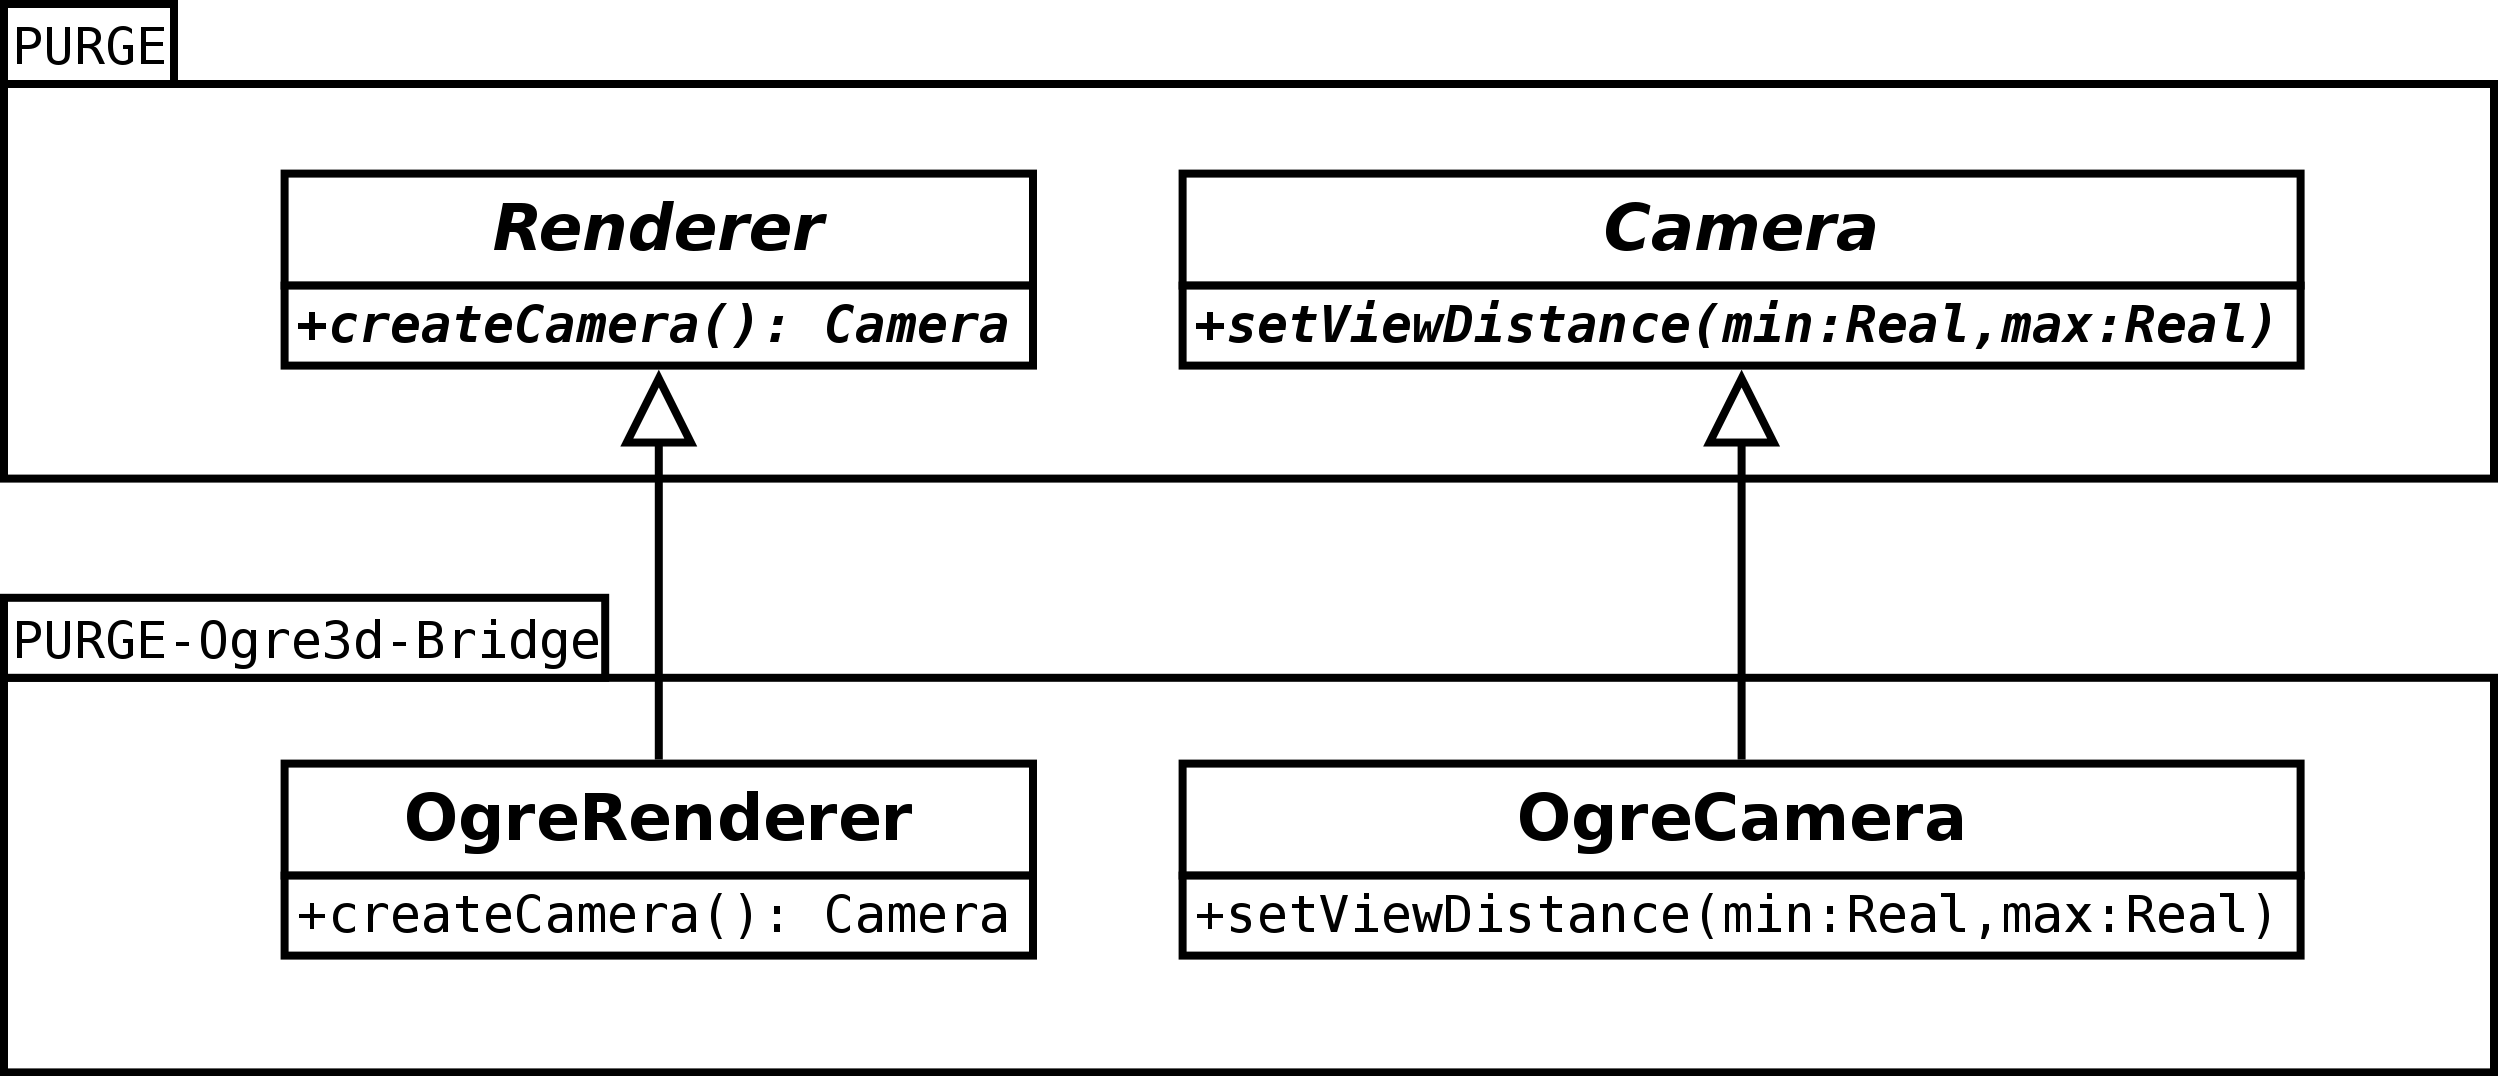
\includegraphics[width=14cm]{images/RendererArchitecture1.png}
		\caption{Initial design approach to the external renderer}
		\label{fig:RendererArchitecture1}
	\end{figure}

	The first approach to the integration of the external render was to design the \classname{Renderer} as an abstract class that is responsible for providing all other objects supported by PURGE, as seen in Figure \ref{fig:RendererArchitecture1}. The drawback of this architecture became clear quite early during the implementation process: The design of PURGE was adopting too many characteristics of the underlying renderer. The library was becoming a layer on top of Ogre3d instead of an independent graphics library.

	To counter this trend during the design process, the architecture was slightly altered to decouple PURGE objects from their implementations in the renderer. The aim was to render the \classname{Renderer} completely interchangeable, even at run-time, an approach to the engine design we have found in \cite{Plummer2004}\footnote{Plummer basically contemplates on a game architecture proposal in \cite{Rollings:2003:GAD:1209229} and attempts to create a game engine with completely interchangeable components for specialized tasks.}. This has lead to the second design outlined in Figure \ref{fig:RendererArchitecture2}, where the objects in PURGE can survive an exchange of the active \classname{Renderer}. We switched from direct inheritance to the bridge pattern as described in \cite{GOF}.

	\begin{figure}[htbp]
		\centering
		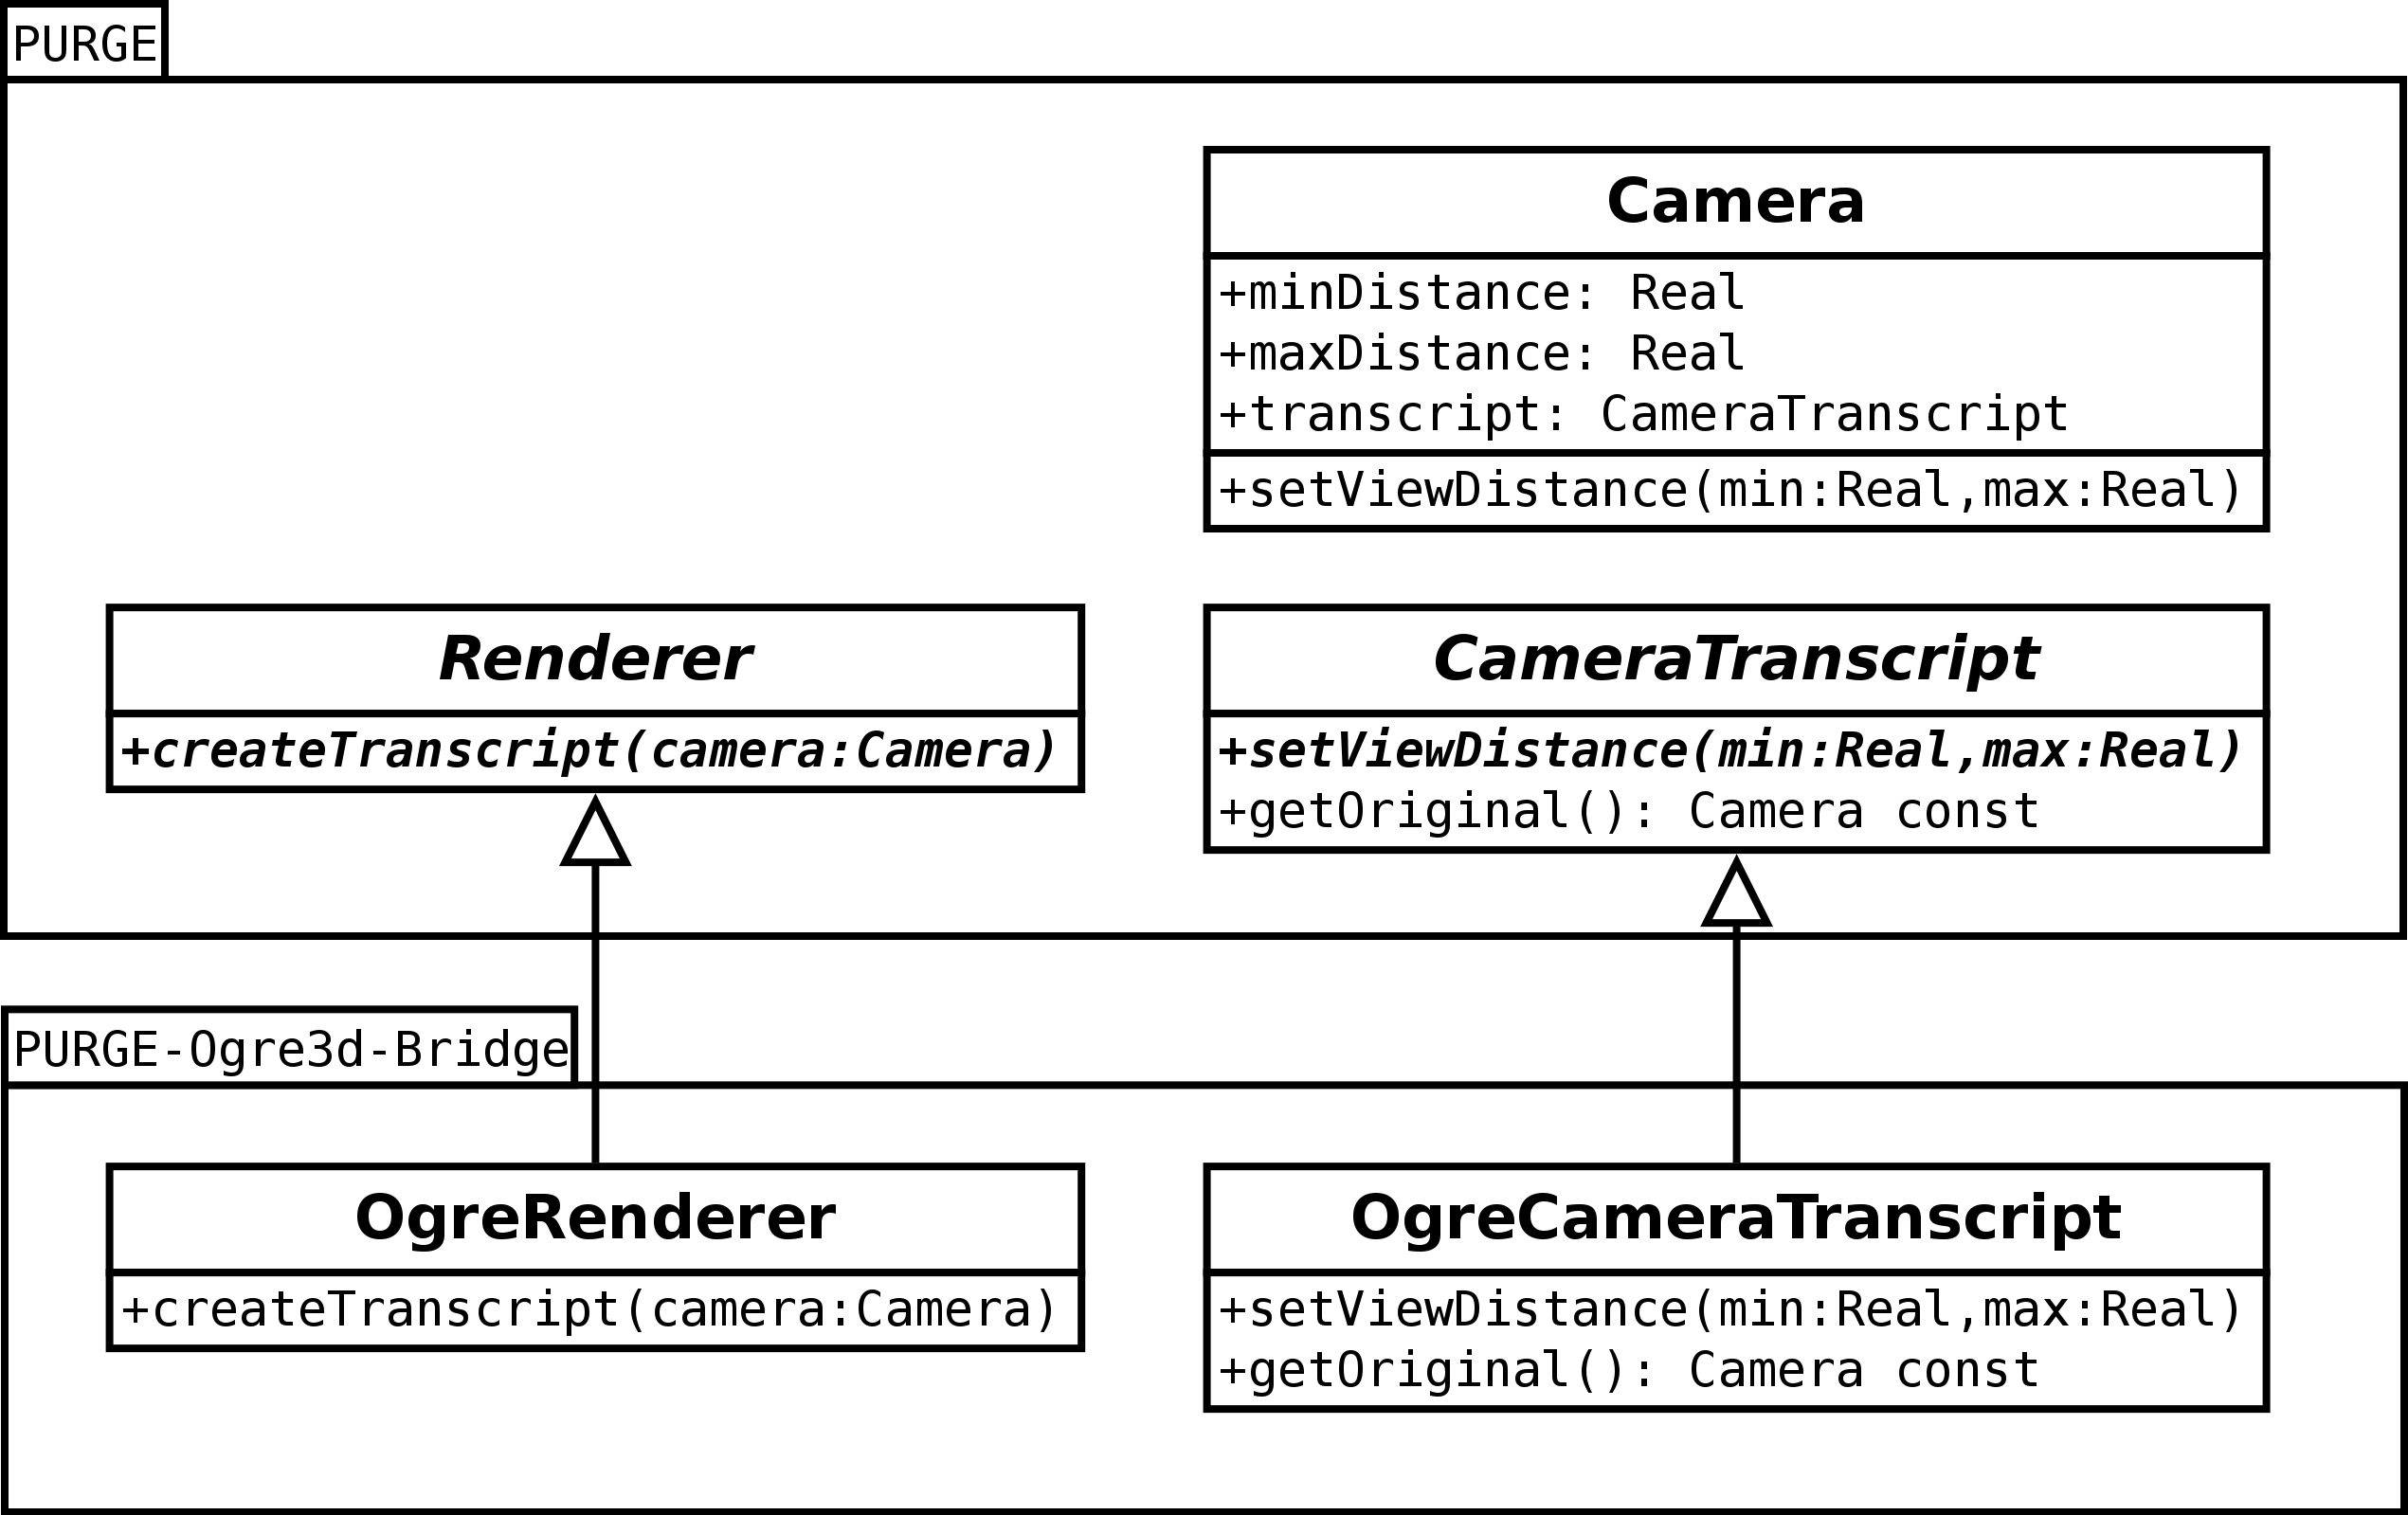
\includegraphics[width=14cm]{images/RendererArchitecture2.png}
		\caption{Second design of the external renderer}
		\label{fig:RendererArchitecture2}
	\end{figure}

	But this change had some drawbacks: Although the PURGE object was now capable of storing its parameters, the API had not changed. The object would now store its state on its own, but immediately update the implementing object. Apart from this lack of solution to the initial problem, another, more grave design flaw was brought to our attention with this switch. Why should the library actually enforce the duplication of the already-present data in the \classname{Renderer}?
			
	What was the \classname{Transcript} good for? It was a required implementation detail in the initial design, but the usage of the bridge pattern had made that class obsolete for PURGE. The \classname{Renderer} was still free to create a mapping of a PURGE-object to its own, graphics-engine specific objects, but PURGE does not need any information from these objects.
	
	So this short-lived solution was discarded and the flow of information was reversed: Instead of pushing any changes from PURGE to the \classname{Renderer}, the \classname{Renderer} is now expected to pull any information it needs from PURGE. The outline of this design can be seen in Figure \ref{fig:RendererArchitecture3}.

	\begin{figure}[htbp]
		\centering
		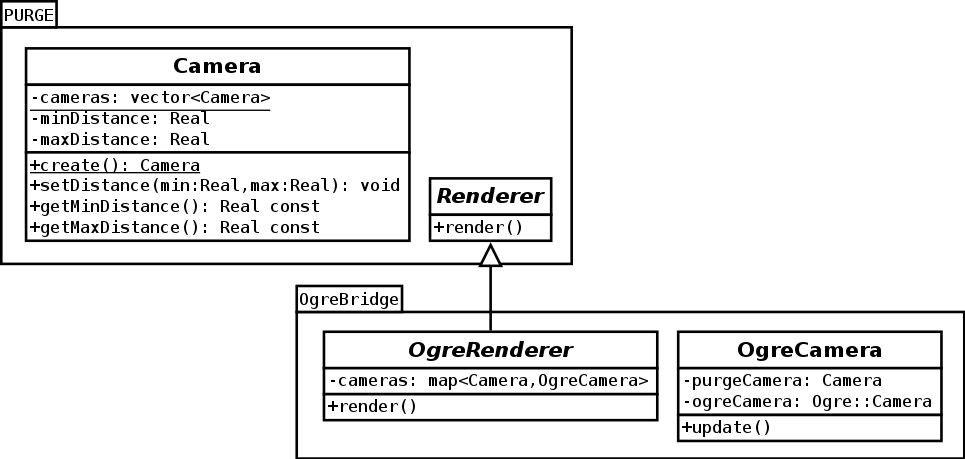
\includegraphics[width=14cm]{images/RendererArchitecture3.png}
		\caption{Third iteration of the renderer architecture}
		\label{fig:RendererArchitecture3}
	\end{figure}

	With this last change, the flow of information is defined as follows:
	
	\begin{numlist}
		\item The application can create, update and delete any number of objects in PURGE. None of the changes have any visible effect at this point.
		\item When all changes for this loop cycle are declared to PURGE, the rendering step initiates.
		\item The \classname{OgreRenderer} is responsible for creating, updating and deleting all required internal objects to render the scene as contained in PURGE.
		\item When the renderer is finished, control is passed back to PURGE, where a new loop cycle begins.
	\end{numlist}

	The implementation of this communication model requires further elaboration on the details of the render loop. We will come back to the implementation specifics in Section \ref{chapter:implementation:renderer}.


	\section{OgreRenderer}
\label{chapter:implementation:ogrerenderer}

	The implementation of the \classname{Renderer} class using the Ogre3d library posed a few interesting problems.

	\subsection{Initialization}

		\subsubsection{Resource Locations}

			PURGE assumes that there is a pool of \classname{Model}s available for usage that can be addressed with a unique string identifier each. Fortunately, Ogre3d takes the same approach: During the initialization of the engine, one has to define a list of resource locations that contain such named objects. This means that the initialization of the \classname{OgreRenderer} itself must provide access to the functionality already present in Ogre3d.

			As this is the only parameter that needs to be specified at the start-up of the engine\footnote{All other parameters can operate with default values, but the location of the resources required by the application are taken to be of great interest to the developer using our API.}, we have decided to accept a resource location as a parameter to the factory.

			Ogre3d supports two different resource location classes containing resources -- both deriving from the \classname{Archive} interface: the \classname{FilesystemArchive} and the \classname{ZipArchive}, one providing access to files in a directory, the other granting access to files in zip-archive. As our library is aimed at rapid prototyping, we have chosen to support a single directory name as a resource location. Additional locations can be added using the API of Ogre3d itself, if required.

		\subsubsection{Delayed Initialization}

			Another issue arose during the implementation of the renderer on Linux. The application was crashing if an Ogre::Camera was created an Ogre::Window. A similar crash occurred when the resource locations were registered before a Window was established. Both issues turned out to be a constraint imposed by OpenGL: Several operations in OpenGL require a window as a context.
			
			The solution was to delay the initialization of the complete \classname{OgreRenderer} until a \classname{PURGE::Window} was defined. This approach has no side effects, as the rendered output on the window is the single duty of the \classname{Renderer}. The method \inlinecode{perform()} would return immediately without performing any operations either way.
			
	\subsection{Communication}

		The communication between the two libraries is handled at a central point, the \classname{Transcription} class, outlined in Figure \ref{fig:Transcription}. This template class uses the curiously recurring template pattern -- just like its management counterpart in PURGE, the \classname{TrackedObject}, outlined in Figure \ref{fig:TrackedObject} -- and provides two static functions for synchronizing PURGE objects and their corresponding bridge objects:

		\begin{figure}[htbp]
			\centering
			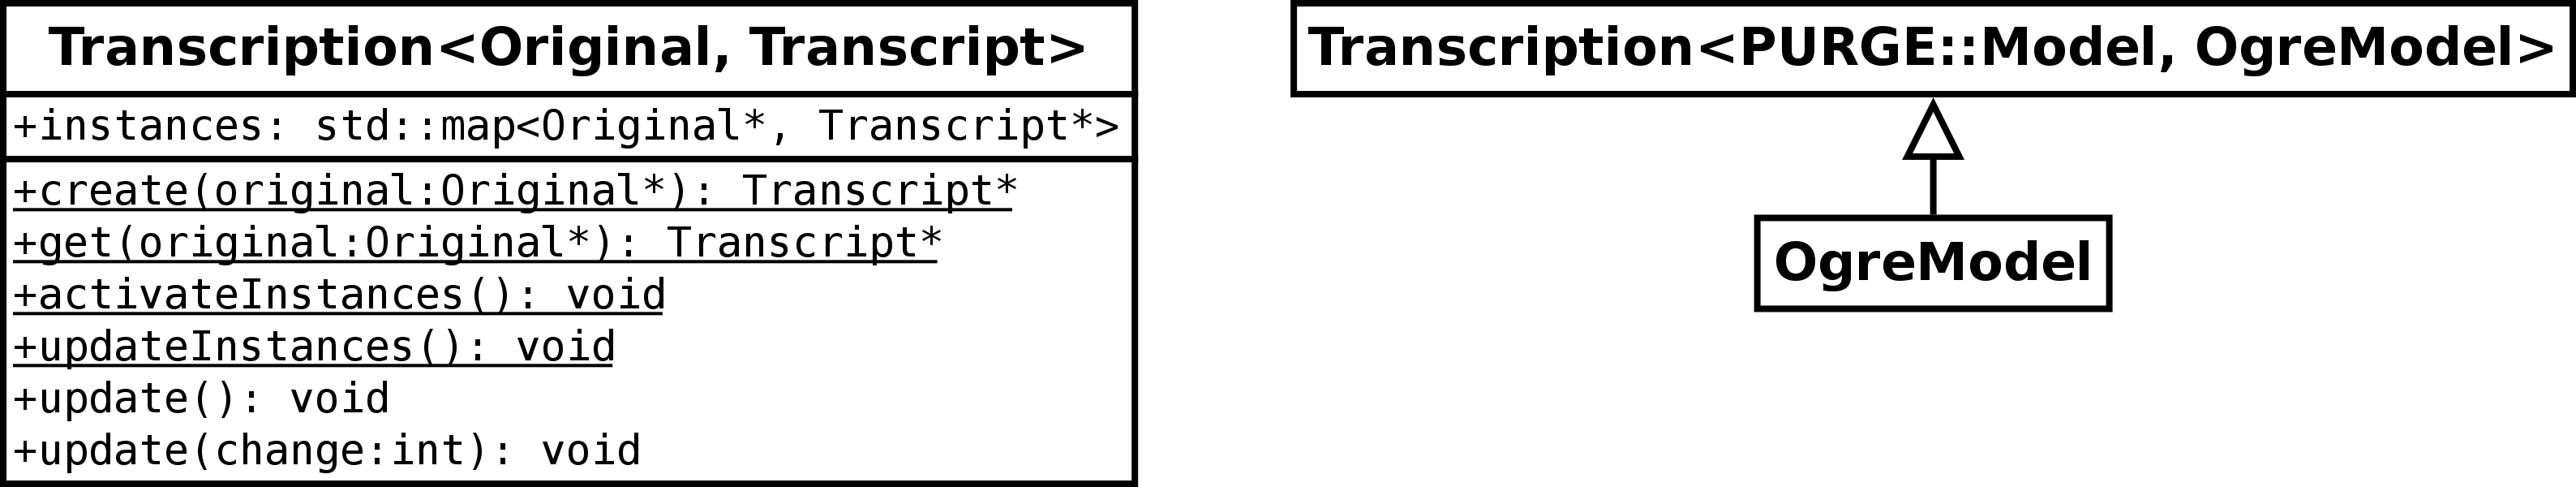
\includegraphics[width=14cm]{images/Transcription.png}
			\caption{The \classname{Transcription} class manages the communication between PURGE objects and Ogre3d objects.}
			\label{fig:Transcription}
		\end{figure}

		\begin{smalllist}
			\item \inlinecode{activateInstances()} will read all available objects in PURGE and create matching instances in the \classname{OgreRenderer}. This step is only necessary to activate the renderer.
			\item \inlinecode{updateInstances()} is called by \inlinecode{OgreRenderer::render()} prior to the rendering. It creates new objects, destroys obsolete objects and carries any modified state from the existing PURGE objects to the bridge objects.
		\end{smalllist}

		Both procedures possibly create bridge objects. To provide greater flexibility for this purpose, the classes assume a static factory method instead of calling the constructor directly. The \classname{Transcript} template parameter has the option of implementing this factory to perform additional operations after the object was created.


	\section{Render Loop}
\label{chapter:design:loop}

	The communication between PURGE and the external \classname{Renderer} is heavily dependent on the render loop -- or main loop -- of our library. The loop basically consists of three different stages that need to be run through repeatedly:

	\begin{numlist}
		\item gathering user input,
		\item updating the scene and
		\item rendering the scene.
	\end{numlist}

	We will be using the ``Single-thread Uncoupled model'' presented by \cite{Valente_Conci_Feijo_2005}, which cycles through these stations periodically in a single thread and updates the objects using the time elapsed since the last cycle. We will see in Section \ref{chapter:implementation:loop}, that the choice of the implementation does not have a strong impact on the API.

	The render loop in a graphics engine must provide an API for the repeated modification of the scene by the application. The sequence described above (gather input, update, render) is present in all reference engines, but each of them approaches this problem quite differently:

	\begin{biglist}
		\item Ogre3d: Provides the FrameListener interface\footnote{http://www.ogre3d.org/docs/api/html/classOgre\_1\_1FrameListener.html} for the registration of recurring tasks during the loop cycle. Developers can implement this interface to react to certain events in the rendering loop, usually the end of the render cycle. The current version provides three such events:

		\begin{smalllist}
			\item \inlinecode{frameStarted()}: Called before the frame is being rendered.
			\item \inlinecode{frameRenderingQueued()}: Called while the GPU is computing the current frame. This event is useful in the case one wants to make use of the CPU at this time, as the CPU would otherwise be idle and the application would block until the GPU is finished.
			\item \inlinecode{frameEnded()}: Called after the rendering is finished.
		\end{smalllist}

		Ogre3d does not have native routines for processing input from external devices (such as keyboards or mice), but an external project is recommended for this purpose throughout the documentation: OIS\footnote{The official web-site of the project is http://www.wreckedgames.com, but more information can be found on its sourceforge project site: http://sourceforge.net/projects/wgois/}. This external library again provides two methods of processing input: buffered and unbuffered. If the library is used in buffered mode, all input can be processed at once during the execution of a frame listener. In unbuffered mode, a listener has to be provided to the library that will be called immediately on the retrieval of new events through system interrupts.

		\item Panda3d: Allows the registration of tasks to be continuously performed at a central facility, the \classname{AsyncTaskManager}. As the name suggests, the library is capable of distributing ongoing tasks across different threads and actually makes use of this mechanism to manage the rendering loop. The rendering step itself is nothing more than a \classname{GenericAsyncTask}. A nice option is the registration of function pointers instead of full-blown classes, which makes playing around with the library a bit more convenient.

		The \classname{AsyncTaskManager} holds multiple instances of \classname{AsyncTaskChain}, which contain objects of type \classname{AsyncTask}. Each \classname{AsyncTaskChain} can run in a separate thread. Furthermore, each \classname{AsyncTask} has a sort number that ensures that tasks can be executed in a predefined order across all \classname{AsyncTaskChain}s. Figure \ref{fig:PandaTasks} visualizes the sequence in a single cycle with two \classname{AsyncTaskChain}s.

		Unfortunately, the name \classname{Chain} is a bit misleading in this context. The name suggests a linear dependence between ``links'', which is not the case: The ``links'' in the chain have additional dependencies to other links in other chains, as seen in Figure \ref{fig:PandaTasks}. A more accurate visual representation of this approach would possibly be ``thread'', reminding of the computational thread it possibly runs in and the thread of a woven fabric, having dependences to other threads.

		\begin{figure}[htbp]
			\centering
			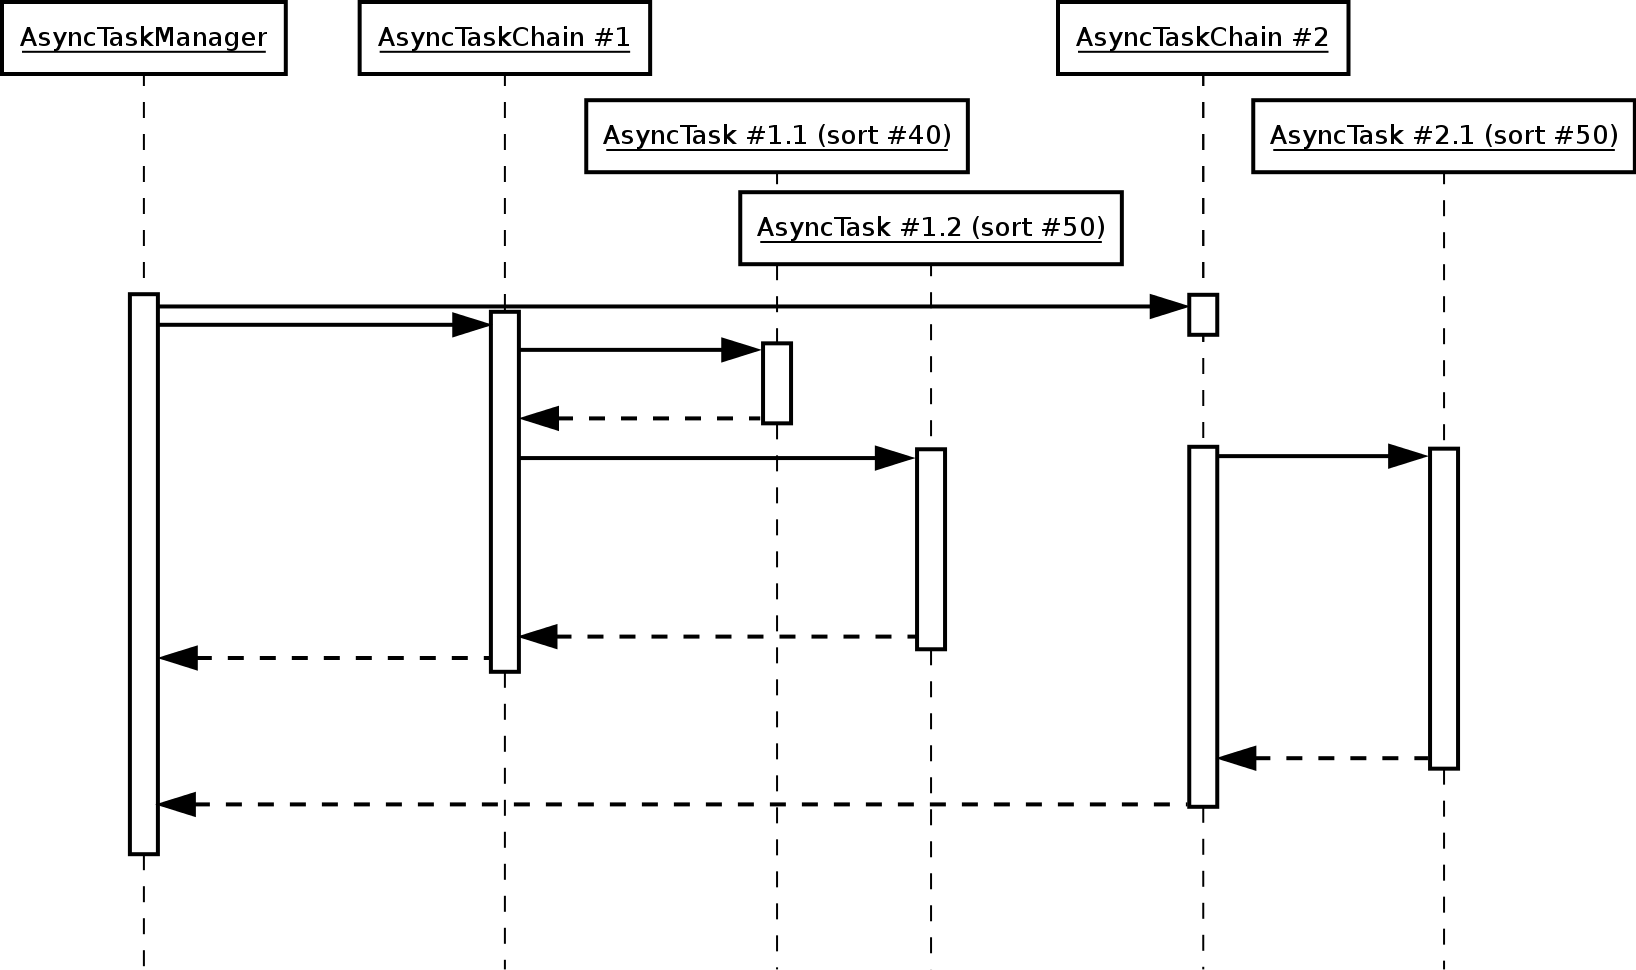
\includegraphics[width=14cm]{images/PandaTasks.png}
			\caption{Simplified sequence diagram of a single rendering cycle in Panda3d. \inlinecode{AsyncTaskChain \#1} and \inlinecode{AsyncTaskChain \#2} start running simultaneously, but the second chain will block until the first task in the first chain was executed, as it has a smaller sort value than the task in the second chain.}
			\label{fig:PandaTasks}
		\end{figure}

		\item OpenSceneGraph: As the project does not provide a render loop \emph{per se}, it is possible to implement ones own loop that takes care of any operations in-between the rendered frames.
			
			But another peculiarity of OpenSceneGraph is the strong focus on the scene graph, even when designing the application flow. We had seen that the scene graph is actually a data structure for organizing objects in space. OpenSceneGraph additionally allows the registration of callbacks to scene nodes. These \classname{NodeCallback}s\footnote{http://www.openscenegraph.org/documentation/NPSTutorials/osgFollowMe.htm} are called during the rendering process as part of the render loop that updates the scene graph.
		
	\end{biglist}

	Among the analyzed libraries, Panda3d provides the most flexible API for managing the scene during the main loop. It allows us to split the loop into multiple threads, making good use of multiple CPUs, but the API emphasizes an early decision which tasks could be performed in separate threads. It requires the definition of \classname{AsyncTaskChain}s for the integration of new tasks into the loop. A dependence between the tasks is then established through the so-called sort numbers.

	An alternative implementation could hide away the details of threading just by introducing Task groups as outlined in Figure \ref{fig:Task}. A Task group adopts the duty of the numeric sort number in Panda3d's loop design. Instead of assigning a value to a task, it is instead added to the same task group as other tasks that can be processed simultaneously.
	
	\begin{figure}[htbp]
		\centering
		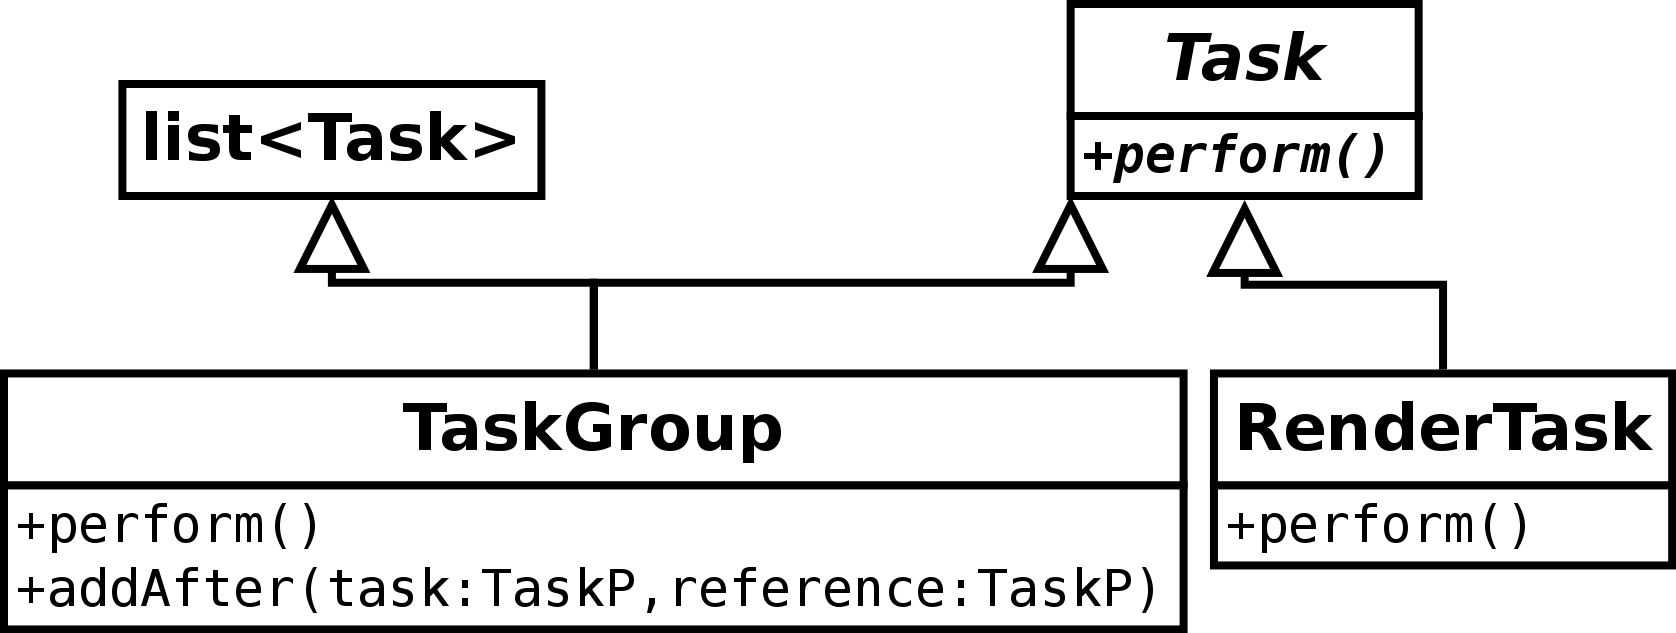
\includegraphics[width=10cm]{images/Task.png}
		\caption{\classname{Task} and \classname{TaskGroup} class hierarchy.}
		\label{fig:Task}
	\end{figure}

	This implementation is in contrast to Panda3d's implementation choice, as it does not group tasks by their ability to run in parallel, but rather creates groups of tasks that need to be performed sequentially -- handling input, computing Physics, computing AI choices, updating positions, and rendering are some examples of such task groups.

	The design described above is equivalent to having a single flat rendering loop that executes tasks sequentially. The \classname{TaskGroup} structure is introduced for convenient re-arranging of the loop elements as a tree structure. With an adequate \classname{TaskGroup} re-implementation it would be further possible to insert parallelism into this design. Although this implementation is not accomplished within this thesis, we will look at it briefly in Section \ref{chapter:implementation:loop}.

	To further simplify the process of adding Tasks to a task group, we will add additional functions to the \classname{TaskGroup} class. These functions will further improve the usability by reducing the number of calls necessary to perform common operations: Adding a task after another reference task, for example.

	While looking into the implementation of the communication between PURGE and the \classname{Renderer} in Section \ref{chapter:implementation:renderer}, we will further discuss the single mandatory task of the library: the \classname{RenderTask}.


	\chapter{Evaluation}
	\label{chapter:evaluation:tests}

We have designed several test scenes to test various aspects of the final API. The tests scenarios are used for obtaining source code metrics, as well as for performance comparison between the implementations with and without the PURGE layer.

All source code measurements exclude statements in reference engines that have no equivalence in the simplified PURGE API. Furthermore, many test scenarios include source code from previous tests. To keep the focus on the current test, all statements that were covered in a prior case are ignored.

The measured values are:

\begin{smalllist}
	\item Lines of code: Number of lines in the source code of the application. Each line contains a single statement, empty lines and lines consisting of a single brace are ignored. Some tests further do not include the placement of a camera, which is required to test the number of rendered frames per second (below), thus the statements required for this positioning are ignored, too.
	\item Function calls: Number of API functions that were used for the implementation.
	\item Distinct function calls: This value represents the number of different functions that were needed to implement the scenario. It is assumed that a lower value reduces the complexity of the API.
	\item Average frames per second: Number of frames that were drawn until the end of the test application. The value is the average of 100 runs of the test scenario, rendering for five seconds in each iteration. It is important to note that this value is highly dependent on the bridge implementation in the case of PURGE.
	\item Peak memory usage: This value is obtained through the \inlinecode{getrusage()} system call on Linux.
\end{smalllist}

\section{Creating a scene}

The first 5 test cases will gradually create an application that will render a space ship at the center of the render window. The finished scene is depicted in figure \ref{fig:TestScene5}

\begin{figure}[htbp]
	\centering
	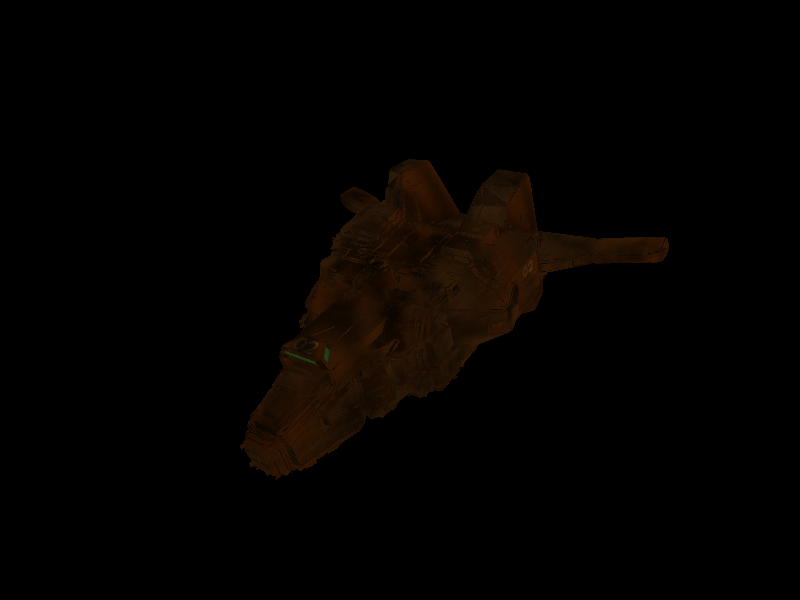
\includegraphics[width=10cm]{images/TestScene5.png}
	\caption{Output of TestScene5}
	\label{fig:TestScene5}
\end{figure}

\subsection{TestScene1: Creating an empty render window}

	The minimal code required to create a window and enter a render loop that will exit whenever the window is closed. This is the most basic scenario for every graphics engine. This test measures the load of the boilerplate code of each graphics library. A performance comparison is not sensible in this case, as PURGE chooses to create a differently sized default render window than Ogre3d.
	
	\begin{table}[htpb]
		\center
		\caption{Code metrics for TestScene1}
		\begin{tabular}{l | l | l | l | l}
			& PURGE & Ogre3d & OpenSceneGraph & Panda3d \\ \hline
			Lines of Code & 2 & 8 & 1 & 4\\
			Function calls & 3 & 9 & 2 & 4\\
			Distinct Function calls & 3 & 9 & 2 & 4\\
		\end{tabular}
		\label{tbl:Code1}
	\end{table}

	Table \ref{tbl:Code1} shows that OpenSceneGraph needs the fewest lines of code for this task. PURGE has two semantically equivalent statements but requires an additional call for the instantiation of the \classname{Renderer}. Additionally this test provides the first assertion of the initial statement that Ogre3d is quite verbose.

\subsection{TestScene2: Controlling the render window}

	In order to create a test scene that allows direct comparison of the frame rates of the same application with and without the PURGE layer, the render window will be adjusted in this test: The render window is centered on the display and created with a predefined size of 800x600 pixels. Panda3d is the only library that did not need the render window object in the initial test case. The results can be seen in Table \ref{tbl:Code2}.

	\begin{table}[htpb]
		\center
		\caption{Code metrics for TestScene2}
		\begin{tabular}{l | l | l | l | l}
			& PURGE & Ogre3d & OpenSceneGraph & Panda3d\\ \hline
			Lines of Code & 1 & 1 & 1 & 3\\
			Function calls & 1 & 1 & 1 & 3\\
			Distinct Function calls & 1 & 1 & 1 & 3\\
		\end{tabular}
		\label{tbl:Code2}
	\end{table}

	This test is the first to additionally measure impact of the added layer to the rendering performance (Table \ref{tbl:Performance2}). As the scene is completely empty (no visible objects have been created), this value shows the resource usage for the idle render loop. This already-low value will further decrease as the impact of the render loop itself is negligible in a graphics application.
	
	\begin{table}[htpb]
		\center
		\caption{Performance metrics for TestScene2}
		\begin{tabular}{l | l | l | l}
			& without PURGE & with PURGE & relative value\\ \hline
			Frames per second & 8726.45 & 8713.35 & 99.85\%\\
			Peak memory usage & 76709 & 77170 & 100.60\%\\
		\end{tabular}
		\label{tbl:Performance2}
	\end{table}

\subsection{TestScene3: Positioning the camera}

	The camera is positioned at \vect{X}{X}{X} and rotated to look at the origin. Panda3d performs all required steps in one statement each:

	\begin{numlist}
		\item retrieving the camera object from the window,
		\item repositioning the camera and
		\item setting the new orientation to look at the global origin.
	\end{numlist}
	
	As OpenSceneGraph provides a method similar to GLU's \inlinecode{gluLookAt()}, the re-alignment can be performed in a single step. PURGE instead makes use of its fluent interfaces to reduce the lines of required code and Ogre3d needs to create a dedicated scene node that performs the transformation for the camera.

	\begin{table}[htpb]
		\center
		\caption{Code metrics for TestScene3}
		\begin{tabular}{l | l | l | l | l}
			& PURGE & Ogre3d & OpenSceneGraph & Panda3d\\ \hline
			Lines of Code & 1 & 3 & 2 & 3\\
			Function calls & 3 & 4 & 5 & 3\\
			Distinct Function calls & 3 & 4 & 5 & 3\\
		\end{tabular}
		\label{tbl:Code3}
	\end{table}

	The repositioning of the camera did not have any impact on the rendering performance, but the tiny gap between the measured memory consumptions closes a bit further as Ogre3d needs to make use of an additional object.

	\begin{table}[htpb]
		\center
		\caption{Performance metrics for TestScene3}
		\begin{tabular}{l | l | l | l}
			& without PURGE & with PURGE & relative value\\ \hline
			Frames per second & 8727.26 & 8712.92 & 99.84\%\\
			Peak memory usage & 76709 & 76934 & 100.29\%\\
		\end{tabular}
		\label{tbl:Performance3}
	\end{table}

\subsection{TestScene4: Loading an object}

	The next step involves loading an object into the scene without modifying its position: the object is attached to the root scene node. As attaching the object to the scene graph is implicit in PURGE, the whole task can be performed in a single step. Ogre3d needs to implement the remaining boilerplate code for registering the location of the resource.

	\begin{table}[htpb]
		\center
		\caption{Code metrics for TestScene4}
		\begin{tabular}{l | l | l | l | l}
			& PURGE & Ogre3d & OpenSceneGraph & Panda3d\\ \hline
			Lines of Code & 1 & 4 & 1 & 2\\
			Function calls & 1 & 6 & 2 & 4\\
			Distinct Function calls & 1 & 6 & 2 & 4\\
		\end{tabular}
		\label{tbl:Code4}
	\end{table}

	The object used for this test consists of approximately 123.000 triangles. We had assumed that the performance difference would decrease in previous tests and this assumption is backed by the performance difference presented in Table \ref{tbl:Performance4}. The memory footprint of the loaded object further reduces the difference in memory consumption.

	\begin{table}[htpb]
		\center
		\caption{Performance metrics for TestScene4}
		\begin{tabular}{l | l | l | l}
			& without PURGE & with PURGE & relative value\\ \hline
			Frames per second & 661.75 & 660.92 & 99.87\%\\
			Peak memory usage & 145362 & 145446 & 100.06\%\\
		\end{tabular}
		\label{tbl:Performance4}
	\end{table}

\subsection{TestScene5: Positioning after loading}

	The previously loaded object is now positioned at the coordinates \vect{-X}{-X}{-X}. Ogre3d and OpenSceneGraph need to create a new scene node that accepts this transformation. A model in Panda3d is itself a scene node that can be manipulated directly. The implementation using PURGE makes use of the fluent interface to append a single function call to an existing line.

	\begin{table}[htpb]
		\center
		\caption{Code metrics for TestScene5}
		\begin{tabular}{l | l | l | l | l}
			& PURGE & Ogre3d & OpenSceneGraph & Panda3d\\ \hline
			Lines of Code & 0 & 2 & 4 & 1\\
			Function calls & 1 & 3 & 4 & 1\\
			Distinct Function calls & 1 & 3 & 4 & 1\\
		\end{tabular}
		\label{tbl:Code5}
	\end{table}

	The additional scene node required by Ogre3d further closes the performance gap between the two implementations, whereas the difference in memory consumption does not change at all.

	\begin{table}[htpb]
		\center
		\caption{Performance metrics for TestScene5}
		\begin{tabular}{l | l | l | l}
			& without PURGE & with PURGE & relative value\\ \hline
			Frames per second & 670.15 & 669.96 & 99.97\%\\
			Peak memory usage & 145361 & 145446 & 100.06\%\\
		\end{tabular}
		\label{tbl:Performance5}
	\end{table}

\section{Completed Scene}

	So far we have looked at the complexity of very specific, incremental tasks. To get a better overview on the amount of code required for the whole scene, we will additionally consider the code metrics of the complete application we have created step by step during the previous five test cases. Table \ref{tbl:Complete5} shows the difference between all APIs.

	\begin{table}[htpb]
		\center
		\caption{Code metrics for the whole TestScene5 implementation}
		\begin{tabular}{l | l | l | l | l}
			& PURGE & Ogre3d & OpenSceneGraph & Panda3d\\ \hline
			Lines of Code & 5 & 19 & 10 & 12\\
			Function calls & 8 & 23 & 14 & 16\\
			Distinct Function calls & 7 & 21 & 14 & 14\\
		\end{tabular}
		\label{tbl:Complete5}
	\end{table}

\section{Modification over time}

	As the previous tests were testing the creation of a single, static scene, we will be looking at some dynamically updated scene graphs in this section.

	\subsection{TestScene6: Movement}

		This scene implements a straight movement of a previously loaded object from one point to another. The presence of the automatic scene node manipulator simplifies this task tremendously in the application using PURGE. The Panda3d API is satisfied with a single function, the other implementations need a separate class for an ongoing modification of the scene. In either case the implementation drives the developer through a lot more knowledge than necessary for such a simple task.

		The metrics just count the amount of effort required to implement this feature into an existing scene. We will only be measuring the statements we needed to write to make the object in TestScene5 move.

		\begin{table}[htpb]
			\center
			\begin{tabular}{l | l | l | l | l}
				& PURGE & Ogre3d & OpenSceneGraph & Panda3d\\ \hline
				Lines of Code & 1 & 8 & 8 & 5\\
				Function calls & 4 & 11 & 12 & 8\\
				Distinct Function calls & 4 & 11 & 12 & 8\\
			\end{tabular}
			\caption{Code metrics for TestScene6}
		\end{table}

		The performance difference between the two implementations was rather small again.

		\begin{table}[htpb]
			\center
			\caption{Performance metrics for TestScene6}
			\begin{tabular}{l | l | l | l}
				& without PURGE & with PURGE & relative value\\ \hline
				Frames per second & 668.50 & 668.22 & 99.96\%\\
				Peak memory usage & 145361 & 145454 & 100.06\%\\
			\end{tabular}
			\label{tbl:Performance6}
		\end{table}

	\subsection{TestScene7: Rotation}

		This test scene implements a 360\degree rotation of an existing object. As with the previous test we will only measure the additional statements required for the rotation. Not surprisingly, the results are very similar to that of the previous test.

		\begin{table}[htpb]
			\center
			\begin{tabular}{l | l | l | l | l}
				& PURGE & Ogre3d & OpenSceneGraph & Panda3d\\ \hline
				Lines of Code & 1 & 10 & 8 & 7\\
				Function calls & 4 & 14 & 11 & 11\\
				Distinct Function calls & 4 & 14 & 11 & 11\\
			\end{tabular}
			\caption{Code metrics for TestScene7}
		\end{table}

		\begin{table}[htpb]
			\center
			\caption{Performance metrics for TestScene7}
			\begin{tabular}{l | l | l | l}
				& without PURGE & with PURGE & relative value\\ \hline
				Frames per second & 670.38 & 670.27 & 99.98\%\\
				Peak memory usage & 145365 & 145458 & 100.06\%\\
			\end{tabular}
			\label{tbl:Performance7}
		\end{table}

\section{Scalability tests}

	The next few tests will probe how the library behaves when the amount of objects increases. As the tests merely add some loops into the previously analyzed code, we will omit the code metrics for the next tests and just look at the performance. To keep the focus further on the CPU-operations, we have performed all tests in this chapter with cubes of size \vect{1}{1}{1}. More complex objects would shift the majority of the execution onto the GPU, which does the exact same operations in both implementations.

	\subsection{TestScene8: Many objects at origin}

		We have created one thousand cubes at the origin of a scene for this test. The Ogre3d implementation attaches all objects directly to the root scene node, whereas the \classname{Renderer} of PURGE creates a dedicated scene node for each object. The results clearly show that these additional scene nodes have a huge impact on the performance in the Ogre3d rendering process. The additional nodes further result in increased memory consumption.

		\begin{table}[htpb]
			\center
			\caption{Performance metrics for TestScene8}
			\begin{tabular}{l | l | l | l}
				& without PURGE & with PURGE & relative value\\ \hline
				Frames per second & 872.94 & 32.84 & 3.76\%\\
				Peak memory usage & 64806 & 68778 & 106.13\%\\
			\end{tabular}
			\label{tbl:Performance8}
		\end{table}

		This is an uncommon use case scene in graphics development, as there are usually very few objects attached to the root scene node. These are the objects that form the immobile environment of the scene -- like the plants and rocks provided by Panda3d's official tutorial application, depicted in Figure \ref{fig:TiltedCamera}. On the other hand, these models can be extremely complex, straining the GPU in another way. To assess these thoughts, we have created the same test scene with a single, complex object, Ogre3d's official ogre head model consisting of 2242 vertices.
		
		\begin{table}[htpb]
			\center
			\caption{Performance metrics for TestScene8.2}
			\begin{tabular}{l | l | l | l}
				& without PURGE & with PURGE & relative value\\ \hline
				Frames per second & 625.87 & 630.57 & 100.75\%\\
				Frames per second (no far-clipping) & 632.73 & 629.06 & 99.42\%\\
				Peak memory usage & 68229 & 68356 & 100.19\%\\
			\end{tabular}
			\label{tbl:Performance8.2}
		\end{table}

		Interestingly, PURGE achieved a higher frame rate in this test. This unexpected difference was caused by the default values of the camera frustum in PURGE: we have disabled the far end of the frustum, always drawing everything in sight. This will generate much worse results with a more populated scene, but we will keep the implication that such a scene will require manual tweaking of the camera parameters, optimizing the API for the simplest scenes. Re-running the application after adjusting the Ogre3d implementation provided the results in Table \ref{tbl:Performance8.2}. We have added this newly found optimization to all following tests.

		The elaboration on the initial test showed that the PURGE software layer has trouble with multitudes of objects positioned at the origin. The same scene could be created in another way that would eliminate this deficit entirely: by merging all models to be positioned at the origin into a single model.

	\subsection{TestScene9: Many objects, distributed in space}

		\begin{figure}[htbp]
			\centering
			
\includegraphics[width=10cm]{images/TestScene9.png}
			\caption{Output of TestScene9}
			\label{fig:TestScene9}
		\end{figure}

		We have created a ``wall'' consisting of $32 * 24 = 768$ cubes facing the camera. The frame rate is again marginally higher with the added software layer, but we couldn't find the cause for this difference in this scene. It is possible that another choice of a default value effects the performance.

		\begin{table}[htpb]
			\center
			\caption{Performance metrics for TestScene9}
			\begin{tabular}{l | l | l | l}
				& without PURGE & with PURGE & relative value\\ \hline
				Frames per second & 37.58 & 37.74 & 100.43\%\\
				Peak memory usage & 67708 & 67702 & 99.99\%\\
			\end{tabular}
			\label{tbl:Performance9}
		\end{table}

	\subsection{TestScene10: Rotating many objects}

		The same objects that were created during the previous test were rotated 360\degree around their up axis throughout the run-time. This test shows that the transmission of changes from PURGE to Ogre3d contains another big performance impact. In contrast to the previous performance deficit in TestScene8, this use case could be much more common and the solution is not as simple.
		
		\begin{table}[htpb]
			\center
			\caption{Performance metrics for TestScene10}
			\begin{tabular}{l | l | l | l}
				& without PURGE & with PURGE & relative value\\ \hline
				Frames per second & 73.96 & 30.38 & 41.08\%\\
				Peak memory usage & 79962 & 83694 & 104.67\%\\
			\end{tabular}
			\label{tbl:Performance10}
		\end{table}

		One possible optimization is sharing of attitude objects. If PURGE has the same handedness of its coordinate system as the underlying graphics engine, it would be possible to write all attitude changes into the quaternion of the underlying engine -- or binding the quaternion used by Ogre3d to the object created by PURGE. The same approach could be applied to other properties (like position and scale) as well. This solution breaks the separation of the two graphic engines in favor of a higher frame rate.

		Taking the idea of such a sacrifice of separation further, we could implement the newly created API for Ogre3d, rather than a dedicated software layer. This would eliminate the need to transmit any changes from one engine to another, leading to much higher performance.

	\subsection{TestScene11: Many objects, with a higher scene graph level}

		The layout of the test with distributed objects was repeated, this time attaching the objects in each row to a common parent node in both implementations. The consistent improvement of the frame rate now starts to indicate a positive impact of our layer on scenes consisting of multiple immobile objects, even after re-running the tests.

		\begin{table}[htpb]
			\center
			\caption{Performance metrics for TestScene11}
			\begin{tabular}{l | l | l | l}
				& without PURGE & with PURGE & relative value\\ \hline
				Frames per second & 40.22 & 40.33 & 100.28\%\\
				Peak memory usage & 67699 & 67698 & 100.00\%\\
			\end{tabular}
			\label{tbl:Performance11}
		\end{table}

		This effect proved to be the result of the model used in the tests. The results changed as we switched from dynamically created cube models to a pre-calculated cube model loaded from a file. The repeated test summarized in Table \ref{tbl:Performance11.1} has slightly lower frame rates than the previous test run, as the pre-calculated cube was larger than the dynamically created one.

		\begin{table}[htpb]
			\center
			\caption{Performance metrics for TestScene11.1}
			\begin{tabular}{l | l | l | l}
				& without PURGE & with PURGE & relative value\\ \hline
				Frames per second & 34.36 & 33.92 & 98.72\%\\
				Peak memory usage & 67700 & 67958 & 100.38\%\\
			\end{tabular}
			\label{tbl:Performance11.1}
		\end{table}

	\subsection{TestScene12: Rotating the scene nodes}

		The scene nodes containing each row are rotated around their ``up'' axis again. % The repeated communication of the state changes causes a performance loss, as in TestScene10.

		\begin{table}[htpb]
			\center
			\caption{Performance metrics for TestScene12}
			\begin{tabular}{l | l | l | l}
				& without PURGE & with PURGE & relative value\\ \hline
				Frames per second & 79.01 & 74.24 & 93.96\%\\
				Peak memory usage & 79966 & 80495 & 100.66\%\\
			\end{tabular}
			\label{tbl:Performance12}
		\end{table}


	\chapter{Conclusion}

	The biggest issue with a learning-by-doing approach in the usage of graphics engines is the huge amount of knowledge their APIs assume. We have managed to create an API that conceals as much of these domain-specific entities as possible and allows the learning developer to choose the order in which he can pick up all these aspects unknown to him.

	We found that we could create whole scenes without the explicit need of scene graphs or quaternions, two areas that were very hard to grasp for us while we were familiarizing ourselves with the reference engines. The wide variety of facades and helper classes further simplified our development process. The code metrics of our tests have shown that half the amount of code is sufficient to perform the exact same basic operations as with other graphics engines.

	The performance of the library is extremely close to that of the original Ogre3d library in most cases. This gap started growing as we started using more primitive objects in our test scenes. This does not come as a surprise, as the whole library was developed for the communication of very abstract concepts.
	
	\section{Future Work}

		We had specifically chosen to cover a very small area of the graphics domain, as the complete domain is huge. Subdividing \classname{Model}s to expose their components -- like meshes or shaders -- is one area that could be interesting. Another approach would be adding interactivity and sound to the library, this could even be sufficient to provide a very simple platform for game development.

		On the other hand, the interaction between PURGE and Ogre3d could be optimized. We had already seen a test case where the implementation with an additional layer can provide even better performance than the original implementation. This is actually quite easy to achieve as one could use much more complex computations in the bridging layer than a layman graphics developer could ever think of.

		Another approach to the optimization could be a stronger coupling to one specific graphics engine, providing a second API to Ogre3d perhaps. PURGE as an additional software layer could be disbanded to just be a part of the rendering library it was using.

		An additional idea emerged during the implementation of the decoupled renderer. The newly created abstraction layer on top of other renderers could be used as a uniform API to the underlying graphics engines. It would be possible to use this API for the comparison of different graphics libraries. This would require more elaborate implementations of the bridging layers, though.



	\appendix
	\bibliographystyle{plain}
	\bibliography{thesis}

\end{document}

